% !Mode:: "TeX:UTF-8"

%%UTF-8
\documentclass[twoside]{nputhesis}
%\documentclass[oneside]{nputhesis}

\usepackage{amsmath}
\usepackage{amsfonts}
\usepackage{booktabs}
\usepackage{multirow}
\usepackage{graphicx}
\usepackage{subfig}
\usepackage{stmaryrd}
\usepackage{standalone}
\usepackage{tabularx} % for 'tabularx' environment
\usepackage[numbers,sort&compress]{natbib}
\usepackage[section]{placeins}

\usepackage{lipsum}

\usepackage{color}

\usepackage{tikz}
\usetikzlibrary{matrix,chains,positioning,decorations.pathreplacing,arrows}

\usepackage{algorithm}
\usepackage{algorithmicx}
\usepackage{algpseudocode}
\usepackage{amsmath}
\usepackage{amssymb}
\usepackage{mathrsfs}
\usepackage{ulem}
\usepackage{bm}
\floatname{algorithm}{算法}
\renewcommand{\algorithmicrequire}{\textbf{输入:}}
\renewcommand{\algorithmicensure}{\textbf{输出:}}
% 增加 \ucite 命令使显示的引用为上标形式
% \newcommand{\ucite}[1]{$^{\mbox{\scriptsize \cite{#1}}}$}
% \newcommand{\upcite}[1]{\textsuperscript{\textsuperscript{\cite{#1}}}}
\newcommand{\ucite}[1]{{\textsuperscript{\cite{#1}}}}
\newcommand{\sWuhao}{\fontsize{10.5pt}{10.5pt}\selectfont}      % 五号, 单倍
\newcommand\equref[1]{公式(\ref{#1})}

\usepackage{enumitem}
\setitemize[1]{itemsep=0pt,partopsep=0pt,parsep=\parskip,topsep=5pt}

\def\final{1} % 1--明评,0--盲评


\usepackage{multirow}
\schoolno{10699}
\classno{TP27}
%\secretlevel{}
\title[A Research on Radar Signal Classification using Deep Learning Based Techniques]{基于深度学习的雷达信号分类算法研究}
\applydate[January 2018]{2018~年~1~月}
\major[Control Theory and Control Engineering]{控制理论与控制工程}

% \support{本文研究得到青年科学基金项目“基于子模优化的远程预警传感器管理研究”(基金编号:61503305)资助。}

\begin{document}
\ifx\final\undefined

\else
    \if\final1
        \author[Zhang Zhishan]{张治山}
        \authorno{2015201518}
        \supervisor[Pan Quan]{潘泉}
    \else
        \author[\hspace{20 mm}]{\hspace{20 mm}}
        \authorno{\hspace{20 mm}}
        \supervisor[\hspace{20 mm}]{\hspace{20 mm}}
    \fi

    \makecover
    \frontmatter
    % 中文摘要
    % 中文摘要
\begin{abstract}
	% 中文 \lipsum[2-3]

	% 摘要——学位论文的简短陈述,应说明该研究工作的目的意义、研究方法、研究成果等,其重点是研究成果,摘要字数一般为硕士论文700~1000字
本文以雷达信号分类识别为主要应用背景,利用深度学习的思想与方法,重点研究了天波超视距雷达地海杂波识别和雷达辐射源识别这两个实际工程问题,具体工作如下:

1)利用天波超视距雷达地海杂波识别结果可以实时准确获得天波雷达的坐标配准修正系数,进而有效提高目标定位精度。
本文在对地海杂波频谱实际数据深入分析的基础上,对原始频谱数据首先进行清洗、裁剪、融合等预处理步骤,然后构建了一个具有六层的深度卷积神经网络分类器并利用具有自适应学习率的算法进行学习,同时结合地海杂波这一实际工程问题对分类阈值进行调整,最后对输出结果以分类精度和与实际地图的匹配精度两个层面进行衡量。
实验结果表明,基于深度卷积神经网络的地海杂波识别算法在电离层环境较差的情况下仍具有较高的识别精度。

2)为了克服大量数据进行标记的成本过高以及部分数据难以人工准确标注的问题,本文进一步提出了基于深度嵌入卷积的地海杂波聚类方法。
通过在地海杂波数据中包含空间、时间信息,添加卷积层、卷积转置层和全连接层,设计了一个以端到端方式训练的卷积自编码器来从未标记的数据中学习特征,并将KL散度与重构损失两部分结合设计了一个新的损失函数。
利用天波超视距雷达的实际地海杂波数据的实验结果表明了深度嵌入卷积聚类算法的有效性。

3)针对复杂电磁环境下辐射源的识别面临的电磁信号干扰大、雷达信号参数相近以及工程中存在未知类别的辐射源等问题与挑战,本文提出了基于深度学习的辐射源个体识别算法。
通过对现有辐射源信号进行分析,利用其模糊函数切片这一脉内细微特征作为训练样本,构建了一个具有10层的一维卷积神经网络作为主分类器来对输入信号做初次分类,其后跟随一个支持向量机分类器作为Meta-Recognition,实现对辐射源中未知类别的辨别。
通过多架飞机的气象雷达辐射源的实际数据证明了本文算法分类的准确性。



	\begin{keywords}
		雷达信号分类, 天波雷达地海杂波识别, 雷达辐射源分类, 深度学习, 卷积神经网络
	\end{keywords}
\end{abstract}
    % 英文摘要
    % !Mode:: "TeX:UTF-8"

% 英文摘要
\begin{Abstract}
Under the background of radar signal classification, this paper focuses on sea/land clutter recognition for Over-the-Horizon Radar(OTHR) and specific emitter identification using deep learning methodology, as follows:


1)The results of OTHR sea/land clutter recognition can be used for coordinate registration, which can help improve the target positioning accuracy effectively.
Based on the analysis of sea/land clutter spectrum data, a six-layer deep convolution neural network classifier is constructed. The original spectrum data is preprocessed by cleansing, trimming, and fusion.
Adaptive Moment Estimation method is used to train the network, which can give a stable learning rate.
As a real-world project, the classification threshold is adjusted according to the features of clutter. The results are evaluated by the classification accuracy and the matching accuracy with actual map.
Experimental results show that the clutter recognition algorithm based on deep convolution neural network still has high recognition accuracy under poor ionospheric environment.

2)In order to overcome the high cost of labeling large amounts of data and the difficult to label some data  accurately manually, this paper further proposed a deep embeddeding convolution method for sea/land clutter clustering.
Spatial locations and time sequences information is added to original clutter spectrum data. The network contains convolutional layer, deconvolutional layer and fully connected layer.
A convolutional autoencoders structure is developed to learn embedded features in an end-to-end way.
The experimental results show the effectiveness of deep embeddeding convolution clustering method.

3)In order to solve the problems of recognizing emitters in similar radar signal parameters and the existence of unknown types emitterin complex electromagnetic environment, this paper proposed a specific emitter identification method based on deep learning.
By analyzing the signal of the specific emitters and using the ambiguity function slice as feature vectors,
a 10-layer one-dimensional convolution neural network is constructed as the primary classifier to classify the input signals firstly. Unknown types of specific emitters are identified by a support vector machine classifier as Meta-Recognition.
The classification accuracy of the algorithm proposed in this paper is high in the experiments of meteorological radars from multiple aircraft.



	\begin{Keywords}
		Radar Signal Classification, Sea/Land Clutter Recognition for Over-The-Horizon Radar, Specific Emitter Identification, Deep Learning, Convolutional Neural Networks
	\end{Keywords}
\end{Abstract}

    \tableofcontents

    \mainmatter
\fi
% 正文内容
 \chapter{绪论}
\section{引言}
而是
\section{天波超视距雷达地海杂波识别}

超视距雷达(OTHR)在高频段运行,能够通过电离层反射检测和定位超过地平线的地区的移动目标,因此在持续监测中起着重要作用\cite{headrick1974over, fabrizio2013high}。 然而,电磁信号通过电离层的传播导致强制性程序,用于目标定位的坐标登记〜(CR),因为地面坐标系中的目标位置(即纬度和经度)是必需的,但是OTHR接收测量 倾斜坐标系〜(即倾斜方位角和倾斜范围)\cite{krolik1997maximum}。 要执行CR,必须调用两个子步骤,(1)为每个测量或目标状态估计选择正确的电离层传播模式,(2)将测量或目标的状态估计从倾斜坐标系转换为地面坐标系。

% In general, a sub-system consists of several ionosondes is deployed and operated with OTHR to provide the information required by CR. The information includes the possible ionosphere propagation modes and the corresponding parameters for each propagation mode, such as the height of each layer of the ionosphere \cite{wheadon1994ionospheric}. OTHR takes such information from ionosondes as the input of it and achieves CR. There are two factors that may deteriorate the localization performance of OTHR using ionosondes. The first one is that the deployment of ionosondes is restricted to available areas. For example, ionosondes can not be deployed in the sea or hostile areas. The ionosphere's parameters of unavailable areas are often obtained by interpolation with those of available areas based on statistical ionospheric models, making the information input into CR inaccurate. The second one is that the independent operation of ionosondes from OTHR results in consistency on the number of propagation modes and inaccuracy on the parameters for each propagation mode. More specifically, the propagation modes recognized by ionosondes may not the same as the propagation modes that the measurements received by the OTHR originate from. Therefore, to reduce the chances of incorrect identification of propagation mode for each measurement or state estimate, and the effect caused by the error of parameters provided by ionosondes so that improve the accuracy of CR, alternative methodologies have to be sought.
一般来说,由OTHR部署和操作的几个离子键合子的子系统提供CR所需的信息。该信息包括可能的电离层传播模式和每个传播模式的相应参数,例如电离层的每层的高度\cite{wheadon1994ionospheric}。 OTHR从Ionosondes获取这些信息作为其输入,并实现CR。有两个因素可能会降低使用离子键的OTHR的定位性能。第一个是离子质子的部署仅限于可用的区域。例如,离子潜能不能部署在海洋或敌对区域。不可用区域的电离层参数常常通过基于统计电离层模型的可用区域插值得到,使信息输入到CR不准确。第二个是来自OTHR的离子键的独立操作导致传播模式的数量和每个传播模式的参数的不准确性一致。更具体地说,离子键的识别传播模式可能不同于OTHR所接收的测量的传播模式。因此,为了减少每个测量或状态估计的传播模式的错误识别的机会,以及由离子质子提供的参数的误差引起的影响,从而提高CR的准确性,必须寻求替代方法。

改善CR的一种方法是使用beacons\cite{weijers1995oth}。 OTHR接收信标发送的信号,并在倾斜坐标系中输出其位置上的测量值。 通过将测量与由GPS提供的地面坐标系中的信标的已知位置进行比较,可以实时地进行CR过程的校正。 然而,信标的使用仅限于可用的区域。 此外,需要对信标进行维护。
% One way available to improve CR is using beacons \cite{weijers1995oth}. OTHR receives the signals transmitted by beacons and outputs the measurements on their locations in slant coordinate system. By comparing the measurements with known locations of beacons in ground coordinate system provided by GPS, correction on the CR process can be carry out in real-time. However, the utilization of beacons is restricted to available areas as well. Additionally, maintenance on beacons is needed.

事实上,另一个来源,海洋/陆地的转变,可以被看作是一种被动的信标,因为海洋和陆地的信号是可以识别的,因为同样的原则是适用的。 使用海岸线的CR的想法首先出现在\cite{wheadon1994ionospheric, anderson1995auto},没有详细的结果报告。 巴纳姆等人\cite{barnum1998over}提出了一种基于海/陆杂波识别的CR方法,主要依靠构造杂波模型。 然而,由于电离层状况的复杂性,海/陆杂乱的特征不稳定,例如海杂波,布拉格峰的主要特征之一可能会偏移甚至失去一个峰值。
% In fact, another source, sea/land transitions, can be regarded as a kind of passive beacons since the same principle is applicable if the signals of sea and land are identifiable. The idea of using coastline for CR is first appeared in \cite{wheadon1994ionospheric, anderson1995auto}, where no detailed results were reported. Barnum~{\emph et. al.} \cite{barnum1998over} proposed a CR method based on sea/land clutter identification, which mainly relies on constructing the clutter model. However, due to the complexity of ionospheric situation, the characteristics of the sea/land clutter is not stable, for example, one of the main features of sea clutter, Brag peak, may shift or even lost one peak.

在本文\cite{cuccoli2009over, cuccoli2009over2, cuccoli2010sea, cuccoli2011coordinate}中,我们提出了一种针对Horizon Sky Wave信号实时坐标注册问题的方法。 该方法是基于对雷达覆盖区域内的海陆过渡位移的先验知识,即利用监视区域的地理形态结构,利用其构建二进制掩模,将其用作 接收的雷达回波的地理参考。 概述了基于收到的雷达回波和二进制杂波签名之间的互相关最大化的地理参考算法,以便指出接收到的信噪比和差分海陆反射散射的最小要求 系数。
% In \cite{cuccoli2009over, cuccoli2009over2, cuccoli2010sea, cuccoli2011coordinate}, In this paper, we propose an approach to the problem of real time coordinate registration for Over the Horizon Sky Wave signals. The approach is based on the a priori knowledge of the displacement of the sea-land transitions within the radar coverage area, namely, takes advantage of the geo-morphological structure of the surveillance area, employing it to build a binary mask to be used as a geographic reference for the received radar echo. The georeferencing algorithm, based on the maximization of the cross-correlation between the received radar echo and the binary clutter signatures, is outlined in order to point out the minimum requirements in terms of received signal-to-noise ratio and differential sea-land backscattering coefficient.

在 \cite{cuccoli2009over2}中,我们最近提出了一种基于对海陆过渡位置的先验知识的天空天空雷达(OTHRsw)的接收到的回波的实时协调注册(CR)的相关方法 在雷达覆盖范围内。 在本文中,我们提出了一种软件仿真工具,用于分析不同OTHR情景中提出的CR方法的性能。 软件工具使用简化的电离层模型和表面杂波雷达相互作用的简化模型来模拟单声道OTH雷达传播。 提出并讨论了假设不同表面杂波场景的仿真结果。
% In \cite{cuccoli2009over2}, We recently proposed a correlation method for the real time Coordinate Registration (CR) of the received echo by Over The Horizon Sky Wave Radar (OTHRsw) based on a priori knowledge of the positions of the Sea-Land transitions within the radar coverage area. In this paper we present a software simulation tool developed to analyze the performance of the proposed CR method in different OTHR scenarios. The software tool simulates the monostatic OTH radar propagation using simplified ionospheric models and simplified models of surface clutter radar interactions. Simulation results assuming different surface clutter scenarios are presented and discussed.

在\cite{cuccoli2010sea}中,我们最近提出了一种基于对海上地位的先验知识的Over Horizon Horizon Wave Radar(OTHR-SW)的接收回波的实时协调注册(CR)的相关方法, 雷达覆盖区内的陆地过渡。 在本文中,我们提出了一个模拟器,可以用于现实OTHR场景中提出的CR方法的性能分析。 假设一个单一的海陆转换场景和一个地理上不变的垂直电子密度分布,提出和讨论了一些模拟结果。
% In \cite{cuccoli2010sea}, We recently proposed a correlation method for the real time Coordinate Registration (CR) of the received echo by Over The Horizon Sky Wave Radar (OTHR-SW) based on a priori knowledge of the positions of the sea-land transitions within the radar coverage area. In this paper we present a simulator that can be used for performance analysis of the proposed CR method in realistic OTHR scenarios. Some simulation result are presented and discussed assuming a single sea-land transition scenario and a geographically invariant vertical electron density profile.

% In \cite{cuccoli2011coordinate}, Cuccoli~{\emph et. al.} studied the problem of range coordinate registration leveraging the geomorphological structure of the surveillance area. The geographical information including coastlines is represented by sea/land binary mask, which is further converted to a reference signal depending on the equivalent ionospheric reflection height. The right equivalent ionospheric reflection height is determined by maximizing the cross-correlation between the received radar echo and the surface mask signatures. However, they assume the OTHR transmits single pulse signals and numerical simulation results are provided.
Cuccoli\cite{cuccoli2011coordinate}等人提出利用监控区域的地貌结构研究范围坐标登记问题。 包括海岸线的地理信息由海/陆二进制掩码表示,根据等电离层反射高度进一步转换为参考信号。 通过最大化接收的雷达回波和表面掩模签名之间的互相关来确定正确的等效电离层反射高度。 然而,他们假设OTHR传输单脉冲信号,并提供数值模拟结果。
% In \cite{cacciamano2012coordinate}, Target detection in Over-The-Horizon (OTH) radars is accomplished by tracking returns in slant range, Doppler and azimuth. Coordinate registration (CR) is the process of localizing the target by converting the slant coordinates to ground coordinates for all the frequencies used in transmission. The CR method uses a 3D ray-tracing algorithm which provides the ground range distance reached with a specific transmission frequency and elevation angle. The ray-tracing approach here adopted uses a 3D electron density model variable with height, latitude and longitude. The ray-tracing output is generally affected by errors due to numerical approximations of the 3D ionosphere model and discretization step used to integrate the differential equations of ray-tracing algorithm. Therefore the raw CR diagram suffers from an error which introduces as a consequence a degradation of target localization accuracy. Accordingly, we propose a coordinate registration technique for OTH sky-wave radars based on 3D ray-tracing that uses the sea-land transitions to mitigate the CR errors. The approach is based on the a priori knowledge of actual group delays relative to the sea-land transition within the area illuminated by the radar antenna beam. The method takes advantage of the geomorphological structure of the surveillance area. The errors introduced by the 3D ray-tracing software are then evaluated by using the actual group delay sat sea-land transitions.Afterwards, the estimated errors are used to correct the coarse CR diagram that was obtained straightforward from the ray-tracing output. Finally, the proposed correction method has been verified under the simplified assumption of a horizontally stratified ionosphere.
在\cite{cacciamano2012coordinate}中,超视距(OTH)雷达中的目标检测通过跟踪倾斜范围,多普勒和方位角的返回来实现。坐标注册(CR)是通过将倾斜坐标转换为传输中使用的所有频率的地面坐标来定位目标的过程。 CR方法使用3D光线跟踪算法,其提供具有特定传输频率和仰角的地面距离距离。这里采用的光线跟踪方法采用高度,纬度和经度的3D电子密度模型变量。射线跟踪输出通常受到三维电离层模型数值近似误差的影响,离散化步骤用于积分光线跟踪算法的微分方程。因此,原始CR图受到误差的影响,导致目标定位精度的降低。因此,我们提出了一种基于3D射线跟踪的OTH天波雷达的坐标配准技术,该雷达使用海陆转换来减轻CR误差。该方法基于对由雷达天线波束照射的区域内相对于海陆转变的实际组延迟的先验知识。该方法利用了监视区域的地貌结构。然后通过使用实际的组延迟饱和海陆转换来评估由3D射线跟踪软件引入的误差。之后,使用估计的误差来校正从射线跟踪输出直接获得的粗略CR图。最后,在水平分层的电离层的简化假设下,验证了所提出的修正方法。

% In \cite{fabrizio2016using}, A skywave over-the-horizon radar (OTHR) can detect and track aircraft or surface targets at ranges of 1000 to 3000 km by reflecting high frequency (HF) signals from the ionosphere. Coordinate registration (CR) is the process of registering OTHR tracks from radar to geographic coordinates. CR is often performed by ray-tracing through a real-time ionospheric model (RTIM). Opportunistic scatterers that produce identifiable radar returns from known reference points (KRPs) may also be exploited for CR. To complement traditional passive KRP sources, this paper investigates the use of uncooperative emitters of opportunity as active KRP sources to enhance OTHR track geo-registration accuracy. A method that utilizes a HF radio broadcast signal as an active KRP source for CR is presented and analyzed using experimental data from the Australian Jindalee OTHR network (JORN).

天文望远镜雷达(OTHR)\cite{fabrizio2016using}可以通过反射来自电离层的高频(HF)信号来检测和跟踪1000到3000公里范围内的飞机或地面目标。 协调注册(CR)是将OTHR轨道从雷达注册到地理坐标的过程。 CR通常通过实时电离层模型(RTIM)进行射线跟踪。 从已知参考点(KRP)产生可识别的雷达回报的机会散射体也可能被用于CR。 为了补充传统的被动KRP源,本文研究了使用不合作的机会发射器作为活动的KRP源来提高OTHR跟踪地理登记精度。 使用澳大利亚金达莱OTHR网络(JORN)的实验数据,提出并分析了利用HF无线电广播信号作为CR的有效KRP源的方法。
% In \cite{turley2013high}, Skywave radar exploit the ionospheric medium to illuminate and track targets at long ranges over vast areas. To achieve optimal performance in the dynamic clutter and noise environment cognitive radar techniques are used to advise waveform parameter and coordinate registration for localisation of targets. Here we introduce an experimental high spatial resolution support-radar that remotely senses surface backscatter clutter. A robust algorithm is described for analysis of the Doppler spectra to determine land or sea backscatter origin. The sensed land-sea interfaces can thus be used for direct registration of nearby targets or assimilation into an ionospheric map.
Skywave雷达利用电离层介质来照射和追踪大范围的远距离目标\cite{turley2013high}。 为了在动态杂波和噪声环境中实现最佳性能,认知雷达技术用于建议波形参数和协调目标定位的配准。 这里我们介绍一个远程感测表面反向散射杂波的实验高空间分辨率支持雷达。 描述了用于分析多普勒频谱以确定陆地或海洋后向散射起源的鲁棒算法。 感测到的陆 - 海界面因此可用于附近目标的直接登记或同化到电离层地图。
% In \cite{coutts2015low}, High fidelity electromagnetic modeling of the wave propagation field is essential to accurately assess the impact of wind-turbine modulated ground clutter on high frequency (HF) Over-The-Horizon (OTH) radar performance. To support the modeling effort, field measurements were conducted in 2014 near the AN/TPS-71 HF Relocatable Over-the-Horizon Radar (ROTHR) in Virginia to investigate wave propagation near the ground. Extensive propagation data were collected by transmitting from a helicopter-borne HF transmitter to a number of monopole antennas on the ground near the ROTHR receive site at three HF frequencies (7.5 MHz, 14.5 MHz, and 23.5 MHz) and various elevation angles from five to zero degrees (grazing incidence) as measured from the receive antenna. The measurement ranges varied from 5 to 40 km and the helicopter altitudes varied from ground level up to 6000 feet. The measurement results are well correlated with model-based predictions for a smooth-homogeneous-earth surface provided that the ¡°effective¡± dielectric constant and conductivity of the terrain are reduced from their expected values as estimated from in situ soil samples and the National Land Cover Database.
对于准确评估风力发电机调制地面杂波对高频(HF)地平线(OTH)雷达性能的影响,波传播场的高保真电磁建模至关重要\cite{coutts2015low}。为了支持建模工作,在2014年在弗吉尼亚州的AN / TPS-71 HF可重定位超地平线雷达(ROTHR)附近进行了现场测量,以研究地面附近的波浪传播。通过从直升机传送的HF发射机到ROTHR接收站附近的地面上的多个单极天线,以三个HF频率(7.5MHz,14.5MHz和23.5MHz)和五个仰角从五个到从接收天线测量的零度(掠入射)。测量范围从5到40公里不等,直升机高度从地面高度变化到6000英尺。测量结果与平滑均质地球表面的基于模型的预测有很好的相关性,前提是地形的“有效”介电常数和电导率从其预期值降低,如从原位土样和国家土地覆盖数据库。

% In \cite{holdsworth2017skywave}, Skywave over-the-horizon radar exploits ionospheric propagation to detect and track targets at long range over vast areas. To achieve optimal performance in the dynamic propagation, clutter and noise environment cognitive radar techniques are used to inform waveform parameter selection and improve coordinate registration for localization of targets. In this paper we investigate the use of Earth surface and infrastructure backscatter to aid in coordinate registration. A transponder was placed in the vicinity of a window turbine farm and a mountain range producing strong backscatter. Terrain echoes are shown to provide similar azimuth-range-Doppler information to the transponder echo with similar temporal coverage. Wind turbine echoes are shown to provide azimuth-range information albeit with less temporal coverage than the transponder and terrain echoes.

Skywave超视距雷达利用电离层传播来检测和跟踪广泛地区的远距离目标\cite{holdsworth2017skywave}。 为了在动态传播,杂波和噪声环境中实现最佳性能,认知雷达技术用于通知波形参数选择,提高目标定位的坐标登记。 在本文中,我们研究使用地球表面和基础设施反向散射来协助协调注册。 一个转发器被放置在一个窗户涡轮机场附近,一个产生强烈反向散射的山脉。 地形回波被显示为具有类似时间覆盖的应答器回波提供类似的方位范围 - 多普勒信息。 风力发电机回波被显示为提供方位角范围信息,尽管它具有比应答器和地形回波更少的时间覆盖。
\section{辐射源类别识别}

辐射源的快速、准确和鲁棒的自动目标识别在现代军事中的作用十分重要,自动目标识别算法需要可以准确区分出已知目标和未知目标,同时可以正确的对于已知目标进行分类。我们需要在未收集大量数据的前提下,可以迅速的识别出新的目标。与传统的利用已知类别的样本进行训练测试的机器学习算法不同,我们这个问题是在Open Set的情况下,将需要考虑将输入识别为未知的情况。本文利用深度卷积神经网络与支持向量机进行结合,以雷达信号的模糊函数作为训练样本,构建了一个可以对未知分类进行识别的分类器。我们利用实际数据进行验证,证明我们的分类器具有很强的准确性。
随着科学技术的进步,现代战场形势瞬息万变,信息对抗在现代军事中的作用越来越重要。纵观整个 20 世纪所爆发的两次世界大战和数次局部战争、21 世纪初的美阿、美伊之战以及最近闹得沸沸扬扬的韩国的萨德事件,无一不昭示着现代战争已成为电子战的“天下”,电子战技术也在历次实战演练中逐渐成熟。电子战也称电子对抗,包括电子侦察、电子攻击和电子防护三个方面。电子侦察主要指从敌方雷达及其武器系统获取有用信息,通过雷达辐射源个体识别,可以对战场环境中敌我双方雷达辐射源的分布情况实施侦察,提供更加全面的、精确的电磁斗争与武器的态势,进行有效的战场指挥与决策,雷达辐射源个体识别已成为当前电子战特别是电子侦察领域的研究热点和难点。然而由于辐射源的特征未知、信号波形日趋复杂、战时电磁环境恶劣,给辐射源的精确识别带来了越来越严峻的挑战。

在雷达辐射源信号特征挖掘方面,己有很多学者作了大量研究工作,在上世纪70年代国外相关研究人员就开始了该部分的研究,该部分研究可以分为两个阶段:
第一阶段为辐射源基本参数特征研究。对于原始信号特征直接求取其载波频率、脉冲宽度、脉冲幅度、到达角度和到达时间等信息,利用其中一个或多个作为特征向量。这种情况主要是应用于电磁环境相对单一、辐射源类别较少、信号形式单一、雷达参数固定的早期。

第二阶段自20世纪90年代以来,西方的军事强国开始研究雷达辐射信号的脉内特征,相继提出了了多种分析雷达信号脉内特征的方法。有代表性的工作有:时域波形分析法、谱相关法、基于专家知识信号处理法、时频综合法、小波分析法、信息理论准则与聚类技术综合法、脉内瞬时频率特征与累积法、信号的分型特征等。

国内对雷达辐射源个体识别技术的研究始于上世纪 80 年代初,虽然起步较晚,但受到了军方的高度重视,在“九五”、“十五”和“十一五”国防预研中给予了大力资助。在脉内特征挖掘方面,毕大平提出易于工程实现的脉内瞬时频率提取技术;张葛祥提出了雷达辐射源信号的小波包特征、相像系数特征、熵特征、粗集理论、信息维数和分形盒维数;朱明提出了基于原子分解的特征、基于Chirplet原子的特征、时频原子特征;普运伟提出了瞬时频率派生特征、模糊函数主脊切面特征;陈稻伟提出了符号化脉内特征、围线积分双谱特征等;余志斌提出的局域波分解、小波脊频级联特征。

另一方面,雷达辐射源识别是一个典型的分类问题,其主要思路为在得到辐射源信号的特征表示之后,借助有效的分类算法来实现特征空间到决策空间的转换,从而确定信号的所属类别。大量的分类算法被成功运用于雷达辐射源识别中,如模板匹配、神经网络、支持向量机等。一般被应用于该领域的有三种分类方法,一种是判别型分类器,其需要在学习过程中最优化某种目标函数;另一种为生成模型分类器,其主要是基于先验概率和类别条件概率密度进行估计,如线性判别分类器、K最近邻等;第三种是决策树分类算法,通过人类专家的先验知识进行分类,如ID3、C4.5算法。

\section{论文研究内容及结构}
\chapter{深度卷积神经网络}
% TODO:深度学习在雷达信号处理中的应用扩展
\section{引言}
\textcolor{red}{看之前的论文,引言先介绍基本问题,然后提出本章的解决方案,最后本章安排}

\textcolor{red}{5518/9500。}

人工神经网络\cite{hebb2005organization}是一种通过模仿大脑神经元行为进行信息处理的数学模型,但由于其无法承受大规模的参数和训练样本并且具有泛化能力差等问题。Fukushima\cite{fukushima1982neocognitron}于1982年首次提出了卷积神经网络模型,Lecun 等人对神经网络传统算法在训练上面临的计算复杂度高等问题进行了改进,提出了基于梯度下降的优化算法\cite{lecun1998gradient}和BP算法\cite{lecun1989backpropagation}。2003年,Simard对卷积神经网络进行了简化\cite{simard2003best}。Hinton 在2006年的两篇文章\cite{hinton2006reducing,hinton2006fast}可以作为深度学习(Deep Learning,DL)正式提出的里程碑。Ciren等人\cite{ciresan2011flexible}在2011年对神经网络进行改造使其可以通过GPU进行训练计算,并在大量的图像数据集对深度学习算法进行了测试,并且都取得了最好的成绩。其在工业界以及学术界掀起了巨大的浪潮,被应用于语音识别\cite{hinton2012deep}、图像识别\cite{krizhevsky2012imagenet}和自然语音处理\cite{collobert2011natural}等各种方面。 专门针对于深度学习的芯片不断问世,例如谷歌公司的TPU\cite{jouppi2017datacenter},大大提高了深度学习的应用场景。
深度神经网络模型是一种非常强大的深度学习模型,他同时可以处理有监督和无监督学习任务。并且随着科技的发展,数据量越来越大,计算机并行能力也有了很大的提高。针对于海量数据,简单的线性模型由于无法充分利用计算能力,不再适用,可以预见在将来会有越来越多的工作应用到深度学习。目前,其内涵已经超出了传统的多层神经网络,甚至机器学习的范畴,逐渐朝着人工智能的方向快速发展\cite{silver2017mastering}。

1982年,Kunihiko等人\cite{fukushima1982neocognitron}首次将卷积神经网络模型的概念引入深度学习。后来许多学者在实践中对CNN的发展和理论分析作出了重大贡献。1989年,LeCun等人将基于梯度的学习方法\cite{lecun1998gradient}和BP算法\cite{lecun1989backpropagation}引入到CNN。2003年,Behnke写了一本总结CNN\cite{behnke2003hierarchical}的书。同年,Simard等人\cite{simard2003best}对卷积神经网络进行了简化。2011年,Ciren等\cite{ciresan2011flexible}进一步改进CNN并实现了GPU版本,使得CNN的训练识别速度有了巨大的提升,并使用CNN框架对多个图像数据库进行实验,并取得了最佳成果。

本章安排如下:2.2节对深度学习的基本分类进行了介绍,2.3节详细地阐述了传统人工神经网络结构的基本定义和神经元之间信息传递的过程,2.4节对本文主要利用的深度卷积神经网络的特性进行了介绍,2.5节进行本章总结。


\section{基本分类}
传统上可以把深度学习分为卷积神经网络(Convolutional Neural Networks, CNN)、递归神经网络(Recurrent Neural Networks,RNN)、长短时记忆网络(Long short-term memory, LSTM)、深度信念网络(Deep Belief NetWorks,DBN)、自动编码器(AutoEncoder)、稀疏编码(Sparse Coding)、限制波尔兹曼机(Restricted Boltzmann Machine, RBM)等。

其中卷积神经网络是最流行的一种深度学习模型,通过使用卷积层极大地减少了中间层的参数数目,使学习效率更高并较少过拟合,同时卷积操作独有的局部感受野(local receptive fields)、共享权重(shared weights)和池化(pooling)三种特性也是处理序列元素分类识别的很重要的一点,权重共享策略减少了需要训练的参数,相同的权重可以让卷积核不受信号位置的影响来检测信号的特性,使得训练出来的模型泛化能力更强;池化运算可以降低网络的空间分辨率,从而消除信号的微小偏移和扭曲。

递归神经网络是一种包含循环的,允许信息持久化的神经网络模型。传统的前馈神经网络中,单独的输入完全确定了余下层的神经元的激活值。而对于递归神经网络,隐藏层和输出层的神经元的激活值不仅由当前的网络输入决定,而且包含了前面的输入的影响。长短时记忆网络是一种特殊的递归神经网络,主要用于解决递归神经网络前期模型难以训练的问题。其通过刻意设计的单元结构,在递归神经网络的基础上添加了元胞状态(cell state)用来保存长期的状态,然后通过门函数来控制此长期状态。

深度信念网络是一个概率生成模型,是由多个限制玻尔兹曼机组成,这些网络被“限制”为一个可见层和一个隐藏层,层间存在连接,但是层内的单元间不存在连接。隐藏单元被训练来捕捉在可见层表现出来的高阶数据的相关性。

通过对于以上几种最常用的深度学习方法的介绍,我们可以发现卷积神经网络是最适合处理本文这种静态类型的数据,循环或者说是不同时刻的输入对于地海杂波类型的识别并没有提高,故递归神经网络和长短时记忆网络显然不适合本问题。另一方面,深度信念网络的生成模型并不关心不同类别之间的最优分类面的位置,故其用于分类问题时,分类精度没有判别模型高。且其学习的是数据的联合分布,相比其他算法具有更高的复杂性。

\section{传统人工神经网络结构}
\textcolor{red}{深度学习在图像识别中的研究及应用——李卫}

\textcolor{red}{这部分需要重新写!!!!}

人工神经网络是一种模拟大脑神经系统的算法,其可以从海量的训练样本中学习到一个权重函数,用来进行模式识别、分类等。神经网络主要是利用将许多个单一神经元(也称作感知器)联结在一起,一个神经元的输出就可以是另一个神经元的输入,形成一个有向无环的网络结构。首先介绍一个神经元的结构,如图\ref{fig:neural}。其神经元具有多个输入$x_1,x_2,\dots $ ,这些输入可以取0和1中的任意值。神经元对于每一个输入有权重$w_1,w_2,\dots $ 和一个总的偏置$b_0$ ,其输出为一个$\sigma(w\cdot x + b)$ ,这里的 $\sigma$为该神经元的激活函数,定义为:
\begin{equation}
  \sigma(z)\equiv\frac{1}{1+e^{-z}}  
\end{equation}
,此处的激活函数称作S型激活函数,常使用的还有$ReLU $ 等激活函数。
\begin{figure}
  \centering
  \includestandalone[width=\textwidth]{figures/neural}
  \caption{神经元}
  \label{fig:neural}  
\end{figure}

\textcolor{red}{多个神经元分层互联可以形成神经网络。图\ref{fig:network}是一个简单的神经网络,其中圆圈表示神经网络的输入,标上$ +1$的圆圈被称为偏置节点,也就是截距项。神经网络最左边的一层叫做输入层,最右的一层叫做输出层(本例中,输出层只有一个节点)。中间所有节点组成的一层叫做隐藏层(不能在训练样本集中观测到它们的值)。同时可以看到,以上神经网络的例子中有3个输入单元(偏置单元不计在内),3个隐藏单元及一个输出单元。
}

\begin{figure}
  \centering
  \includestandalone[width=\textwidth]{figures/network1}
  \caption{神经网络}
  \label{fig:network}  
\end{figure}

\textcolor{red}{本例中网络的层数为 $ n_l=3$ ,将第 $ l $层记为 $ L_l$ ,于是$  L_1$ 是输入层,输出层是 $ L_{n_l} $。本例神经网络有参数 $ (W,b) = (W^{(1)}, b^{(1)}, W^{(2)}, b^{(2)}) $,其中 $ W^{(l)}_{ij}$ (下面的式子中用到)是第 $ l $层第 $ j$ 单元与第 $ l+1 $层第$  i$ 单元之间的联接参数(其实就是连接线上的权重,注意标号顺序),$ b^{(l)}_i $是第$  l+1 $层第$  i$ 单元的偏置项。因此在本例中, $ W^{(1)} \in \Re^{3\times 3}$ , $ W^{(2)} \in \Re^{1\times 3}$ 。注意,没有其他单元连向偏置单元(即偏置单元没有输入),因为它们总是输出 $ +1$。同时,我们用 $ s_l $表示第$  l$ 层的节点数(偏置单元不计在内)。}

$ a^{(l)}_i$ 表示第$  l $层第 $ i$ 单元的激活值(输出值)。当$  l=1$ 时,$  a^{(1)}_i = x_i $,也就是第$  i $个输入值(输入值的第 $ i$ 个特征)。对于给定参数集合$  W,b $,我们的神经网络就可以按照函数 $ h_{W,b}(x)$ 来计算输出结果。本例神经网络的计算步骤如下:
\begin{align}
a_1^{(2)} &= f(W_{11}^{(1)}x_1 + W_{12}^{(1)} x_2 + W_{13}^{(1)} x_3 + b_1^{(1)})  \\
a_2^{(2)} &= f(W_{21}^{(1)}x_1 + W_{22}^{(1)} x_2 + W_{23}^{(1)} x_3 + b_2^{(1)})  \\
a_3^{(2)} &= f(W_{31}^{(1)}x_1 + W_{32}^{(1)} x_2 + W_{33}^{(1)} x_3 + b_3^{(1)})  \\
h_{W,b}(x) &= a_1^{(3)} =  f(W_{11}^{(2)}a_1^{(2)} + W_{12}^{(2)} a_2^{(2)} + W_{13}^{(2)} a_3^{(2)} + b_1^{(2)}) 
\end{align}
 $ z^{(l)}_i $表示第$ l $层第$  i$单元输入加权和(包括偏置单元),比如,$  z_i^{(2)} = \sum_{j=1}^n W^{(1)}_{ij} x_j + b^{(1)}_i$ ,则$  a^{(l)}_i = f(z^{(l)}_i) $。

这样就可以得到一种更简洁的表示法。这里激活函数 $ f(\cdot)$ 扩展为用向量(分量的形式)来表示,即$  f([z_1, z_2, z_3]) = [f(z_1), f(z_2), f(z_3)]$ ,那么,上面的等式可以更简洁地表示为:

\begin{align}
z^{(2)} &= W^{(1)} x + b^{(1)} \\
a^{(2)} &= f(z^{(2)}) \\
z^{(3)} &= W^{(2)} a^{(2)} + b^{(2)} \\
h_{W,b}(x) &= a^{(3)} = f(z^{(3)})
\end{align}

将上面的计算步骤叫作前向传播。用$  a^{(1)} = x$ 表示输入层的激活值,那么给定第$  l$ 层的激活值 $ a^{(l)}$ 后,第 $ l+1$ 层的激活值 $ a^{(l+1)}$ 就可以按照下面步骤计算得到:

 \begin{align}
z^{(l+1)} &= W^{(l)} a^{(l)} + b^{(l)}   \\
a^{(l+1)} &= f(z^{(l+1)})
\end{align}

将参数矩阵化,使用矩阵-向量运算方式,我们就可以利用线性代数的优势对神经网络进行快速求解。

也可以构建另一种结构的神经网络(这里结构指的是神经元之间的联接模式),也就是包含多个隐藏层的神经网络。最常见的一个例子是 $  n_l$ 层的神经网络,第$   1 $层是输入层,第$   n_l$ 层是输出层,中间的每个层 $  l$ 与层 $  l+1$ 紧密相联。这种模式下,要计算神经网络的输出结果,我们可以按照之前描述的等式,按部就班,进行前向传播,逐一计算第 $  L_2 $层的所有激活值,然后是第$  L_3$ 层的激活值,以此类推,直到第 $  L_{n_l}$ 层。这是一个前馈神经网络的例子,因为这种联接图没有闭环或回路。

神经网络也可以有多个输出单元。比如,图\ref{fig:network2}的神经网络有两层隐藏层:$  L_2 $及 $ L_3$ ,输出层$  L_4 $有两个输出单元。

\begin{figure}
  \centering
  \includestandalone[width=\textwidth]{figures/network2}
  \caption{具有多个输出单元的神经网络示意图}
  \label{fig:network2}  
\end{figure}

要求解这样的神经网络,需要样本集  $ (x^{(i)}, y^{(i)})$ ,其中 $ y^{(i)} \in \Re^2$ 。
\section{深度卷积神经网络}
卷积神经网络(Convolution neural network,CNN)是深度学习中的一种重要算法,在分类等很多领域具有很大的优势。该方法经常被用于图像识别、语音识别等问题。它对原始数据进行卷积运算,\textcolor{red}{然后提取从最后一步生成的卷积数据的特征},丰富了识别中使用的特征。同时,它可以通过池化(合并相邻特征)减少计算复杂度。
深度卷积神经网络与传统人工网络的两个主要区别是其具有超过两个的隐藏层以及可以逐层初始化模型的参数。其通过更多的隐藏层可以更好的对事物的特征进行学习表达。典型的卷积神经网络由深层结构堆叠在一起的多个不同的层组成:输入层,多组卷积和池化层,有限数量的完全连接的隐藏层,以及输出层。其中最主要的部分为卷积层。其利用输入数据中的局部结构,将整个输入空间划分成很小的隐藏单元。将各个隐藏单元的权重构建得到的卷积核作用于整个输入空间,从而得到特征向量。利用这种机制,我们不仅大大减少了参数数量同时提高了数据的平移不变性。
  
其基本架构如图\ref{fig:cnn_network}所示,最左边的为输入层,其中的神经元为输入神经元。最右边的输出层包含有输出神经元,可以有一个也可以有多个。中间层为隐藏层,这部分为需要进行主要设计,也是各种神经网络模型的主要区别之处。为了增强其泛化能力,一般情况下有扩增路径(将多个分支包含在架构中)、金字塔形状(在整个架构中应该有一次整体的平滑的下采样,而且该下采样应该与信道数量的增长结合起来)、规范层输入(使层输入标准化,使所有输入样本更加平等)等各种设计法则,此部分需要根据实际问题以及测试结果不断调整。

\textcolor{red}{对于卷积神经网络的模型进行引用,同时修改图}
\begin{figure}
  \centering
  \includestandalone[width=\textwidth]{figures/cnn_network}
  \caption{深度卷积神经网络示意图}
  \label{fig:cnn_network}  
\end{figure}

\subsection{卷积}
\textcolor{red}{该部分如何miaoshu}

深度卷积神经网络在特征提取过程中一个主要操作为卷积,在前向计算过程中,对于输入的一定区域的数据$x$和滤波器(或者说权重)$w$ 点乘后得到新的特征向量,然后滑过一个个滤波器,组成新的输出数据$s(t)=\sum_{a=-\infty}^{\infty}x(a)w(t-a) $。每个滤波器只关心数据的部分特征,当出现它学习到的特征的时候,就会呈现激活态。

深度卷积神经网络在特征提取过程中一个主要操作为卷积,在前向计算过程中,对于输入的一定区域的数据$x$ 和滤波器(或者说权重)$w$ 点乘后得到新的特征向量,然后滑过一个个滤波器,组成新的输出数据$s(t)=\sum_{a=-\infty}^{\infty}x(a)w(t-a)$ 。每个滤波器只关心数据的部分特征,当出现它学习到的特征的时候,就会呈现激活态。

\subsection{局部感受野}
\textcolor{red}{对于传统的神经网络,每个输入元素会连接到每个隐藏神经元。相反,我们只是把输入的频谱数据进行小的、局部区域的连接,也即第一个隐藏层中的每个神经元会连接到一个输入神经元的一个区域。这个输入向量的区域被称为隐藏神经元的局部感受野。它是输入向量上的一个小窗口,对于每个连接学习一个权重而隐藏神经元同时也学习一个总的偏置。通过在整个输入频谱数据上交叉移动局部感受野,可以构建起第一个隐藏层。
}

\subsection{共享权重和偏置}
上面已经说过对于每个隐藏神经元具有一个偏置和连接到它的局部感受野的权重,同时对于该层的所有的隐藏神经元中每一个使用相同的权重和偏置。也即,对第$j$个隐藏神经元,输出为:
$\sigma(b+\sum_{m=1}^M w_m a_{j+m}) $
这里$\sigma$是神经元的激活函数,$b$是偏置的共享值,$w_m$是一个共享权重的$1\times M$向量,$a_k$表示位置$k$的输入激活值。\textcolor{red}{这意味着第一个隐藏层的所有神经元检测完全相同的特征,只是在输入频谱数据的不同位置,因此卷积网络可以很好地适应频谱数据的布拉格峰偏移情况。}

\subsection{池化}
我们在通过卷积获得了特征之后,下一步我们希望利用这些特征去做分类。理论上讲,人们可以用所有提取得到的特征去训练分类器,例如Softmax分类器(多分类的逻辑回归分类器),但这样做面临着计算量的挑战,除此以外过多的特征向量,也容易导致过拟合。

深度卷积神经结构具有过拟合的自然趋势,虽然可以通过权重共享来减少参数的数量。但是由于大多数情况下,估计集的数量比训练集大一个数量级,使得神经网络模型的泛化能力不足。在每个训练迭代中,每个隐藏单元以预定概率被随机删除,删除后学习过程继续。这些被称作$dropout$的随机扰动有效地防止了神经网络学习过程的依赖关系,并在隐藏的单元之间创建了复杂的关系。这样增加了网络模型的复杂度,从而提高深度神经网络模型的泛化能力。
\subsection{激活函数}
激活函数的选择是构建卷积神经网络模型的一个非常重要的方面。正如前一节所述,传统的神经网络模型中通常选择Sigmod或双曲正切作为激活函数。\textcolor{red}{介绍ReLU的优越性,同时修改公式表示方法}。然而,我们通常在卷积神经网络中使用以下ReLU激活函数。
\begin{equation}
F(x) = max (0, x)
\end{equation}
ReLU具有优于传统激活函数的几个优点:更快的计算速度和更有效的梯度传播(它们不像S形单元那样饱和),生物学可能性和稀疏激活结构。尽管它们结构简单,但仍然保持足够的辨别性质。其缺点之一是随机权重的初始状态,多个单位可能过早地落入死区(零输出的恒定梯度)。因此,当与整个连接层进行全连接时,Sigmod激活函数的效果更好。
\begin{equation}
F(x) = \frac{1}{1-e^x}
\end{equation}

\textcolor{red}{画出三种激活函数的曲线图}
\begin{equation}
  F(x)=tanh(x)=\frac{e^x-e^{-x}}{e^x+e^{-x}}
\end{equation}
\subsection{网络的训练与学习}
\textcolor{red}{添加文字描述,关于梯度下降算法。}

如果用符号$x $表示一个训练输入,用$y=y(x) $ 表示对应的期望输出。学习算法的主要目的是找到一个权重$w$和偏置$b$使得网络的输出$y(x) $ 可以拟合所有的训练输入$x$ 。为此可以定义一个损失函数(又称作代价函数):
\begin{equation}
  C(w,b)\equiv \frac{1}{2n}\sum_x||y(x)-a||^2 
\end{equation}
这里$w$表示所有的网中权重的集合,$b$ 是所有的偏置, $n$是训练输入数据的个数,$a$ 是表示当输入为$x$ 时输出的向量,求和总是在总的训练输入$x$ 上进行的。上述损失函数为均方误差,其是可以根据不同的问题进行不同的设置的。从定义可以看出, $C(w,b) $越小说明分类越准确,那么训练神经网络的目的就是找到最小化二次代价函数 $C(w,b) $的权重和偏置。
\begin{figure}
	\centering
	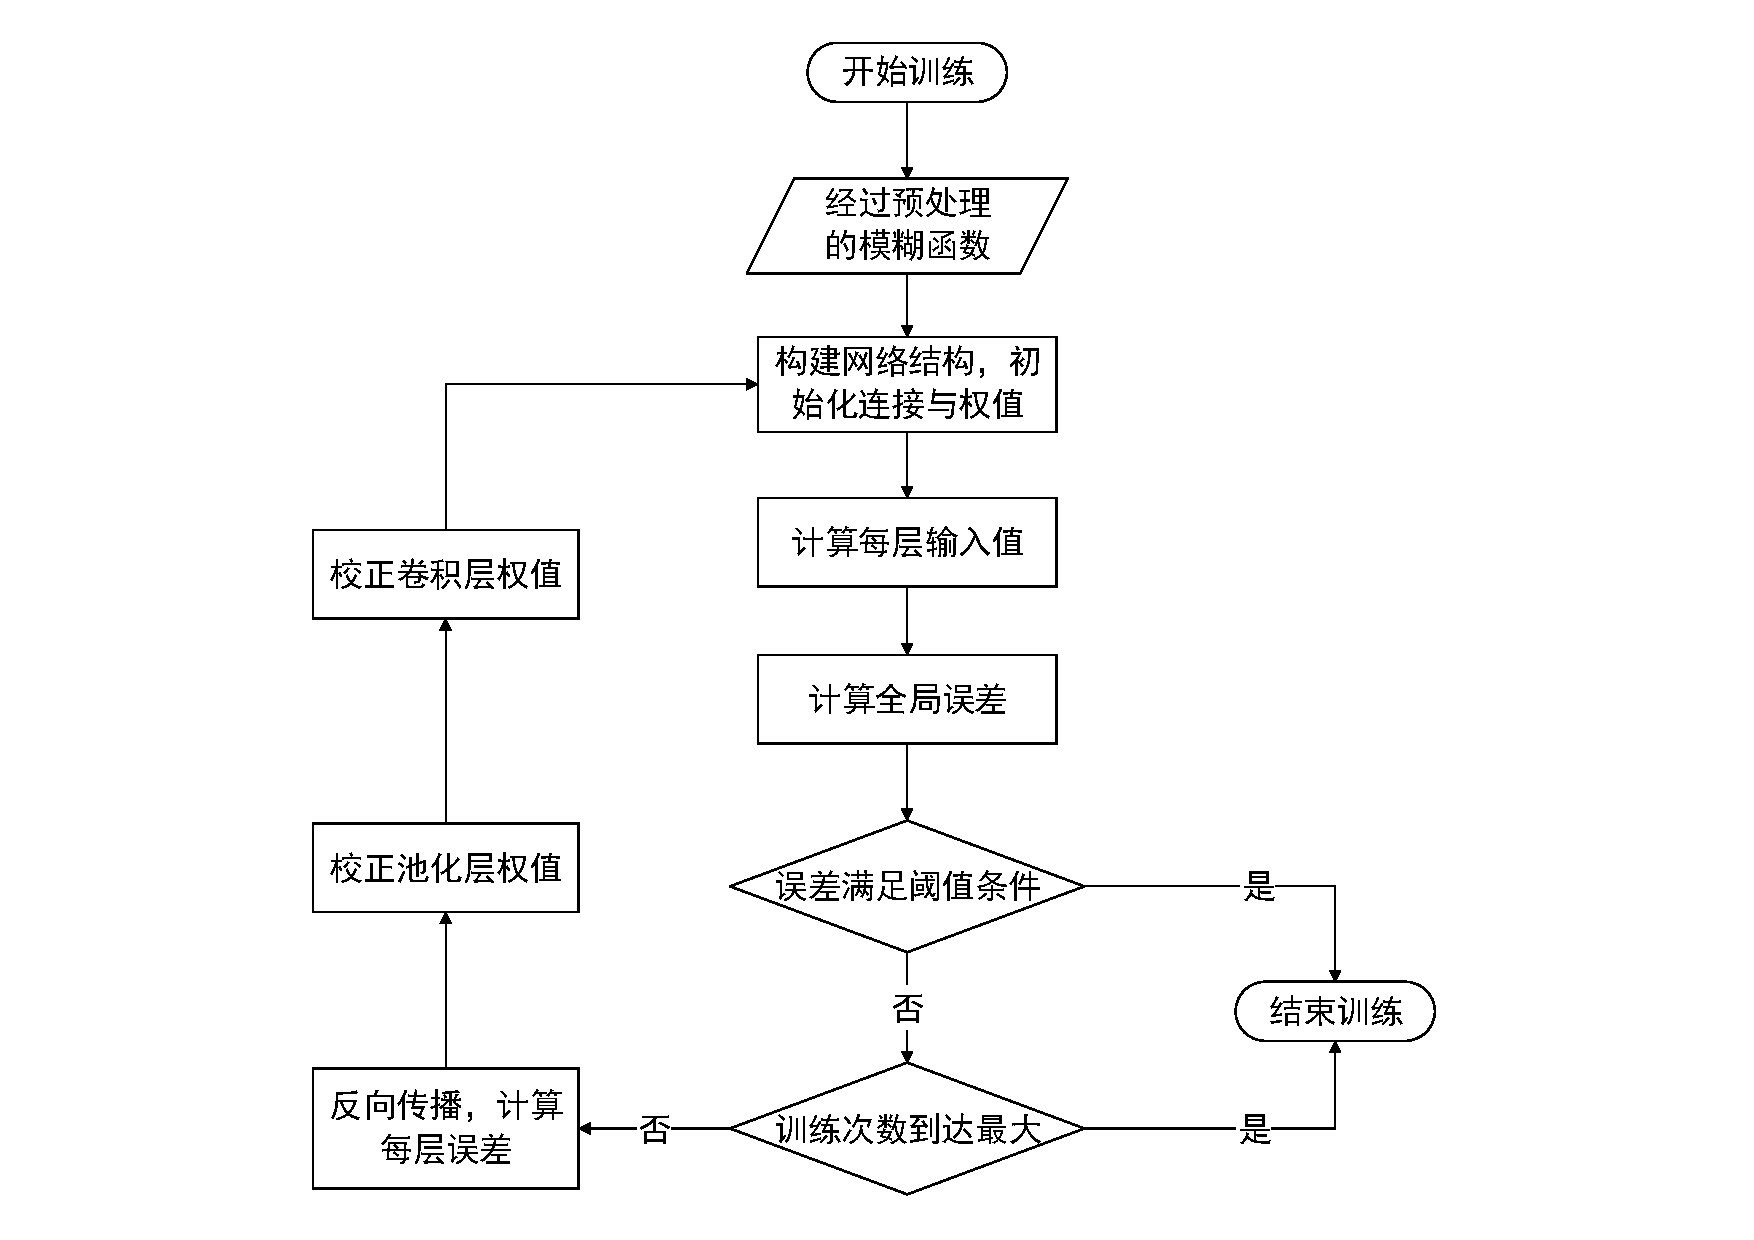
\includegraphics[width=\textwidth]{figures/cnn_flow.pdf}
	\caption{深度卷积神经网络算法训练流程图}
\end{figure}
将上述问题一般化也就是,最小化任意的具有 $m $个变量的多元实值函数 $C(v) $, $v=v_1,v_2,\dots,v_m $。对于这种具有大量变量的函数的解析解是极其复杂的,其比较合理的思路为利用数值计算的方法求取其极值点。每次对于$C $ 中的自变量 添加一个微小的变化$\Delta v $ ,根据此变化反映出来的$C $ 的变换 $\Delta C $更新下次的微小变化,从而使得$C $ 可以持续减小。对$C $ 中自变量的变化$\Delta v=(\Delta v_1,\dots,\Delta v_m)^T $ , $\Delta C $将会变为
\begin{equation}
    \Delta C \approx \bigtriangledown C \cdot \Delta v   
\end{equation}
,这里的梯度$\bigtriangledown C $ 定义如下:
\begin{equation}
\bigtriangledown C \equiv (\frac{\partial C}{\partial v_1},\dots,\frac{\partial C}{\partial v_m})^T 
\end{equation}
其把$v$的变化关联为$C$的变化,假设我们选取
$\Delta v=-\eta \bigtriangledown C $
这里的$\eta $是学习率,一般取一个很小的正数,这时候有
\begin{equation}
\Delta C \approx -\eta\bigtriangledown C\cdot\bigtriangledown C=-\eta||\bigtriangledown C||^2 \leq 0  
\end{equation}
也即如果利用更新规则
$v \rightarrow v'=v-\eta \bigtriangledown C$,
$C $会持续减小,此更新规则即为梯度下降算法,这就是最基本的学习算法。可以根据选择不同的代价函数 $C $或者通过计算来完成学习速率的选择等各种技术对学习算法进行优化。

% \begin{figure}[H]
% 	\centering
% 	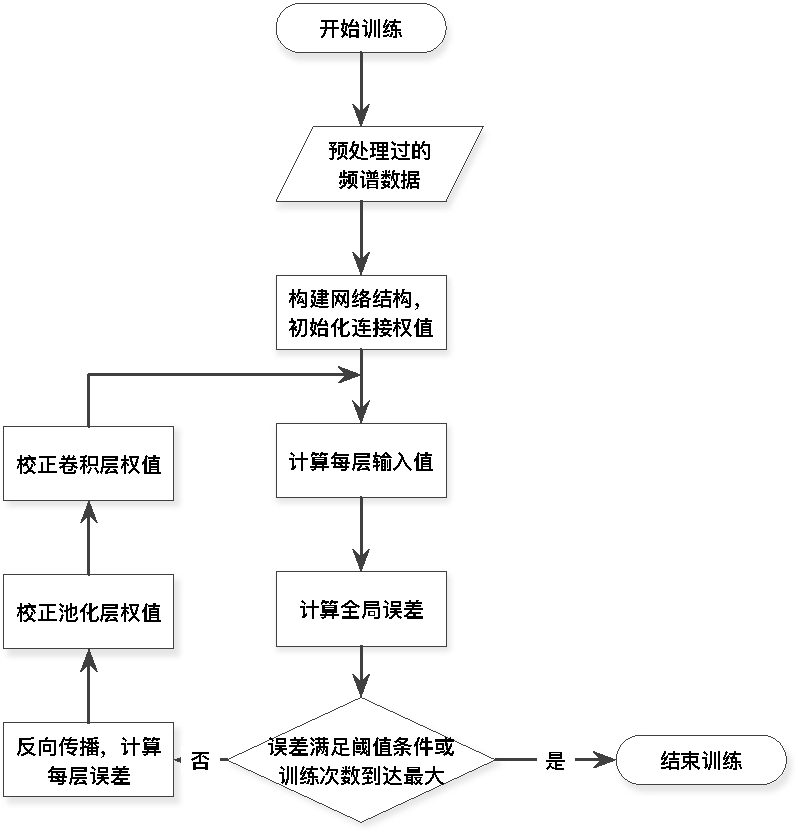
\includegraphics[width=\textwidth]{figures/train}
% 	\caption{深度卷积神经网络训练过程图}
% 	\label{fig:train}
% \end{figure}

\section{小结}
本章介绍了深度学习的相关基础。首先是其基本分类,然后针对于本文利用的深度卷积神经网络,介绍了传统的神经元的结构和卷积神经网络基于此的改进。在最后讨论了深度卷积神经网络在雷达信号处理中的应用。
% \begin{table}
%  \caption{测试表格}
%  \centering
%  \begin{tabular}{cccccc}
%    \toprule
%    & $h$ & $L^2$ error & Order & $L^{(\alpha,\beta)}$ error & Order \\
%    \midrule
%    \multirow{5}{4em}{$\alpha=0.85$\\ $\beta = 0.85$}
%    & 1/4   & 3.8571e-04 &      - & 3.0781e-03 &      -\\
%    & 1/8   & 1.3035e-04 & 1.5651 & 1.2640e-03 & 1.2840\\
%    & 1/16  & 3.8665e-05 & 1.7533 & 5.2782e-04 & 1.2599\\
%    & 1/48  & 4.9386e-06 & 1.8731 & 1.5519e-04 & 1.1142\\
%    \bottomrule
%  \end{tabular}
% \end{table}


 \chapter{基于深度学习的天波超视距雷达地海杂波识别}
\section{引言}
% \textcolor{red}{该章可以添加利用二维卷积神经网络进行识别的算法实验}
% \textcolor{red}{复合类的提取}

天波超视距雷达目标定位精度依赖于传播模式的准确识别以及坐标配准系数的精确测量。电离层传播的复杂性使得传播模式很难精确确定,而电离层探测子系统独立于主雷达工作导致其提供的坐标配准参数与主雷达量测回波存在不一致性、误差大等问题,从而造成电离层传播模式识别正确率低、目标定位精度差等。天波超视距雷达地海杂波识别是一种基于无源信标(远海区域的岛屿等陆地)获得坐标配准系数的技术。鉴于远海地区有源设备的布置面临着较大的困难,通过区分识别地海杂波、构建地海边界轮廓、与先验地理轮廓信息匹配可同样提供坐标配准修正参数,改善周围航迹目标的定位精度。受分辨率低、定位精度差、系统偏差大、电离层多模、多路径传播等因素影响,天波雷达地海杂波识别技术存在很大挑战,主要体现在以下几个方面:
\begin{itemize}
	\item 天波雷达的距离分辨率为$7.5-30$公里,方位分辨率为$0.582-1.067$度,低分辨率影响地海特性的判别以及匹配精度;
	\item 电离层状况变化情况十分复杂,导致地海杂波的特性并不稳定,区分地海杂波特性的Bragg峰会发生偏移甚至某个峰会消失,对地海杂波的建模影响很大,传统的建模方法一般根据实际数据选取一种分布来描述雷达杂波,如瑞利分布、威布尔分布、K分布等。但天波超视距雷达获得的杂波模型一直变化,这种建模方法不能得到很好的结果;
	\item 传统的地海杂波的分类特征很难定量描述。一个熟练的操作人员可能很熟练地区分出地海杂波,但是这部分却很难利用数学模型对其描述;
\end{itemize}

本章提供了一种新的在复杂的电离层环境下的基于深度神经网络的地海杂波识别技术,避免了对杂波进行建模选取特征的方法,从根本上避免了传统方法所面临的困难。构建了适用于天波超视距雷达地海杂波类型识别的卷积神经网络,利用大量训练数据对卷积神经网络进行训练,提取合理的特征;然后,利用提取的特征对实时雷达地海杂波回波进行在线分类识别。我们利用不同电离层条件、雷达工作条件、位置和时间下的频谱数据对我们所提出的算法进行了验证,实验结果证明我们的算法大大提高了天波超视距雷达地海杂波的识别正确率与实时性。

本章安排如下: 3.2节对天波超视距雷达地海杂波信号进行了分析,并对数据集进行分组,3.3节构建了本章的基于深度学习的分类器,详细阐述了根据实际数据的特性构建分类器的过程,3.4节利用实际数据对于本章的分类器与已有方法进行对比,验证了本章提出方法的性能,3.5节进行本章总结。

\section{地海杂波频谱数据分析}
对于一般的进行天波雷达地海杂波识别的文章,其主要利用海杂波的Bragg特性,但是在实际情况中,受电离层条件、工作环境等的影响,会出现很多频谱很难分辨的情形,如图\ref{fig:spectrum}所示。
\begin{figure}[H]
	\centering
	\subfloat[地杂波频谱]{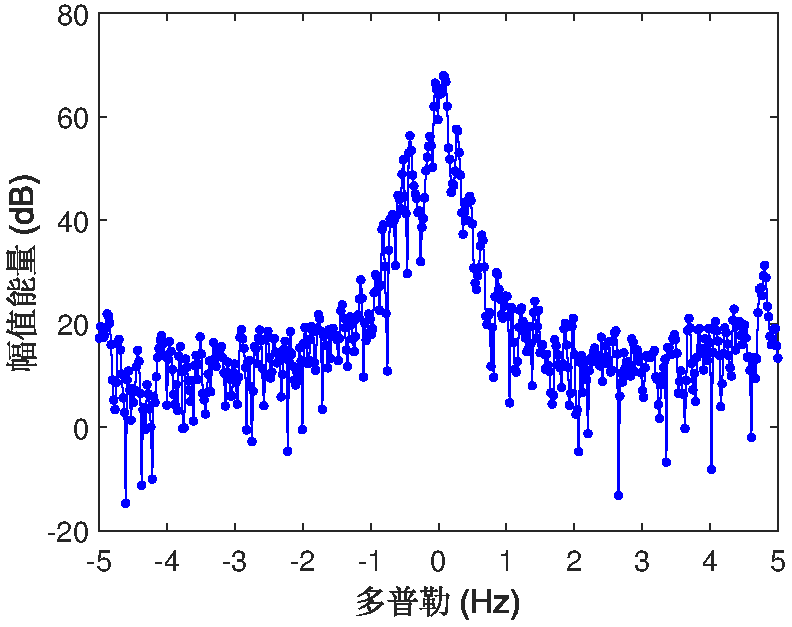
\includegraphics[width=6.67cm]{figures/othr/land}%
		\label{fig:land}}
	\hfil
	\subfloat[海杂波频谱]{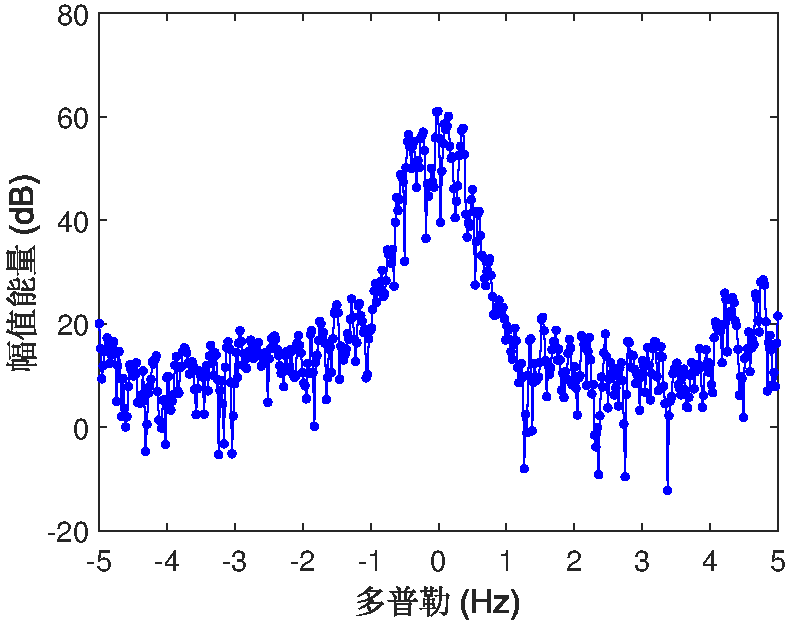
\includegraphics[width=6.67cm]{figures/othr/sea}%
		\label{fig:sea}}
	\caption{两幅无法轻易区分的地海杂的频谱波示意图。图 \ref{fig:land} 的Bragg峰具有小的频偏,图 \ref{fig:sea} 作为海杂波却无法容易的分辨出Bragg峰.}
	\label{fig:spectrum}
\end{figure}
在天波超视距雷达的工作过程中,不同的时间和地理位置对应于不同的电离层条件,不同的电离层条件将严重影响频谱的状态。对于不同的雷达工作条件,由于发射频率变化,回波频谱密度和幅度也将随之变化。通过观察、学习大量不同条件的频谱数据,可以更全面地区分地海杂波。

在本章的问题中,我们选取了几种不同的雷达工作配置(工作频率、朝向等)下的数据。多普勒频率的范围可以是-5Hz至5Hz,也可以是-20Hz至20Hz。我们分别以不同的频率训练数据。此外,对于相同频率的数据,我们通过人工辨识的方法从中抽取出可以准确判定为地或者海的样本数据用于实验的训练和测试。同时,为了保证样本的多样性,对于同一个雷达参数下的数据,我们根据季节、地理位置、一天的早中午进行了选择,确保可以覆盖尽可能多的情形。

我们所有的数据都来自不同时间,不同地点和不同雷达配置的频谱数据。我们分析了所有频谱数据,并选择一些典型的频谱数据,如图\ref{fig:classical_spectrum}所示。

\begin{figure}[H]
	\centering
	\subfloat[杂波干扰严重的频谱图]{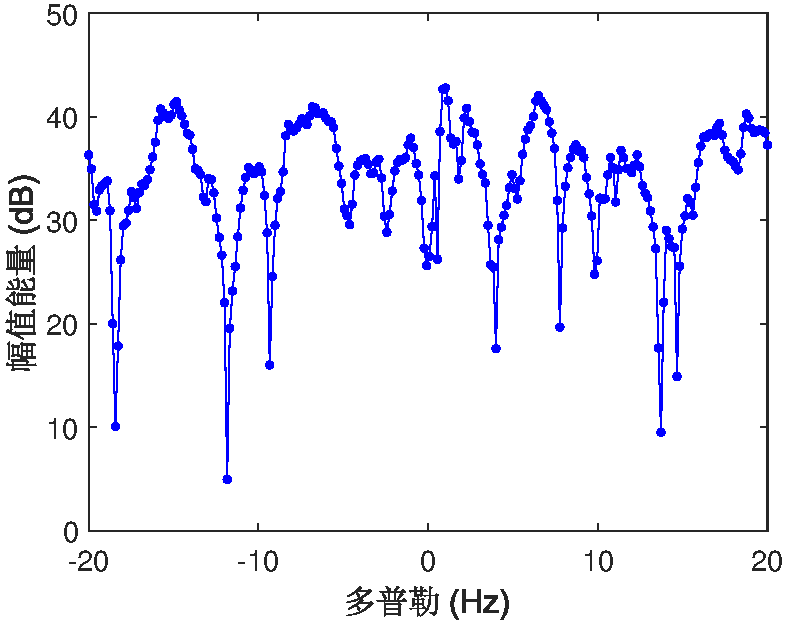
\includegraphics[width=6.67cm]{figures/othr/noise}}%
	\hfil
	\subfloat[具有较强展宽的频谱图]{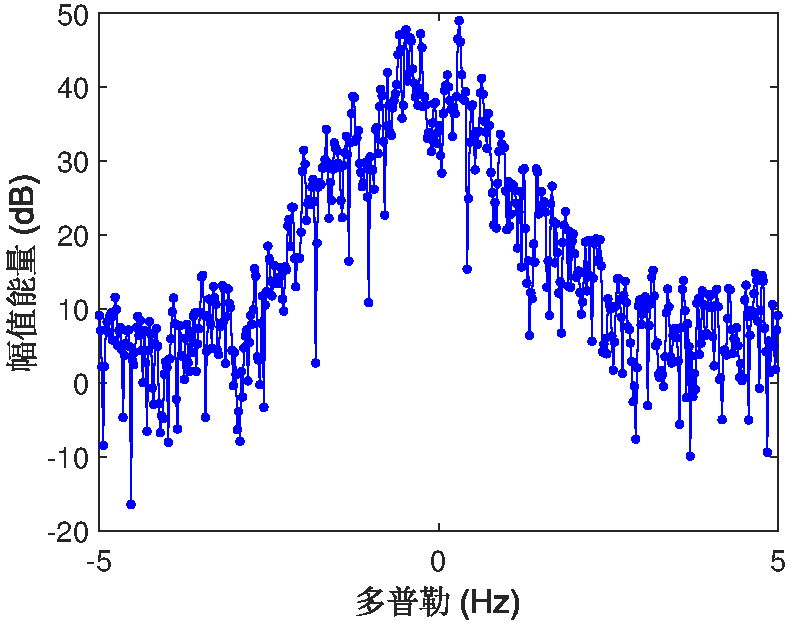
\includegraphics[width=6.67cm]{figures/othr/wide}}%

	\subfloat[Bragg峰缺失频谱图]{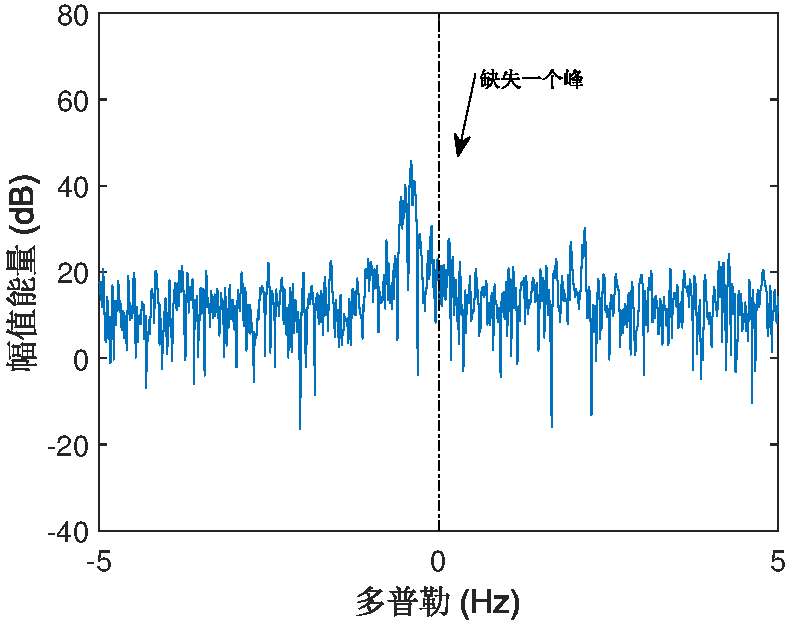
\includegraphics[width=6.67cm]{figures/othr/lost}}
	\hfil
	\subfloat[Bragg峰偏移频谱图]{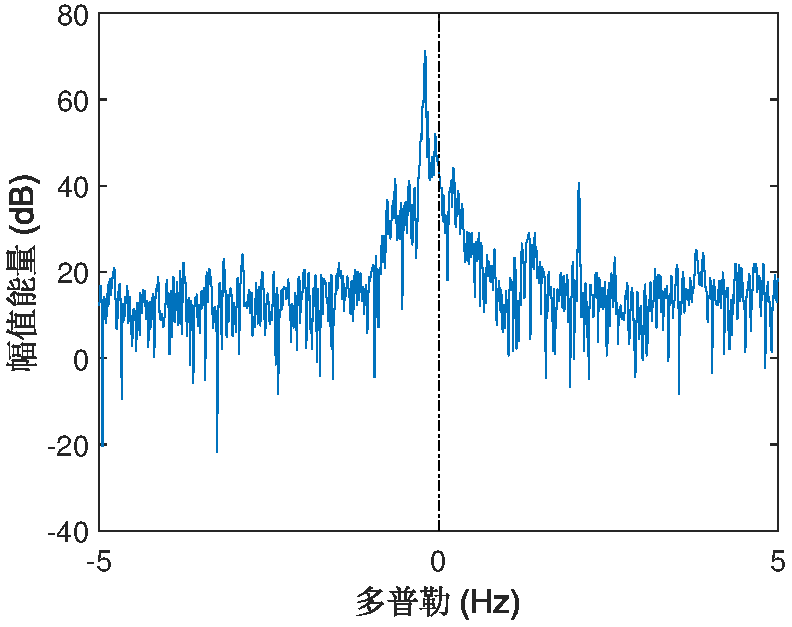
\includegraphics[width=6.67cm]{figures/othr/shift}}

	\subfloat[对空工作模式频谱图]{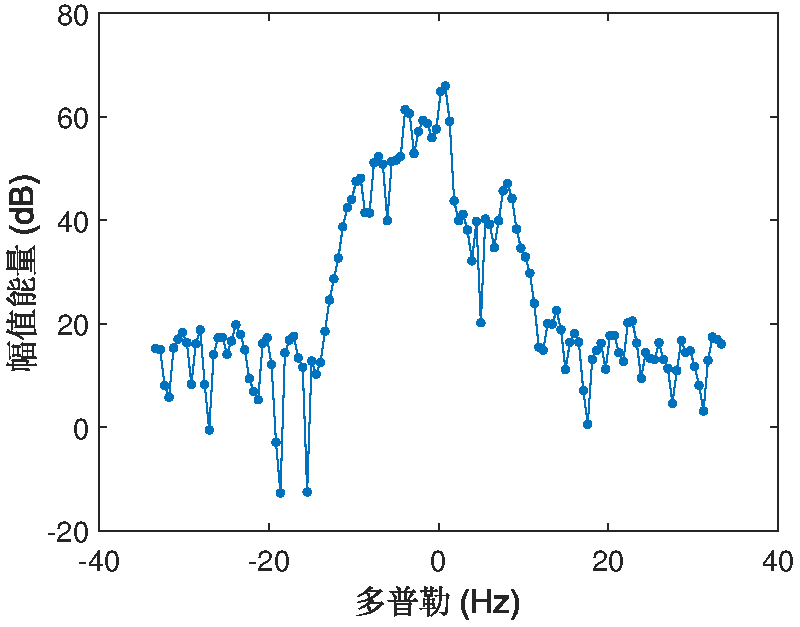
\includegraphics[width=6.67cm]{figures/othr/sky}}
	\hfil
	\subfloat[对海工作模式频谱图]{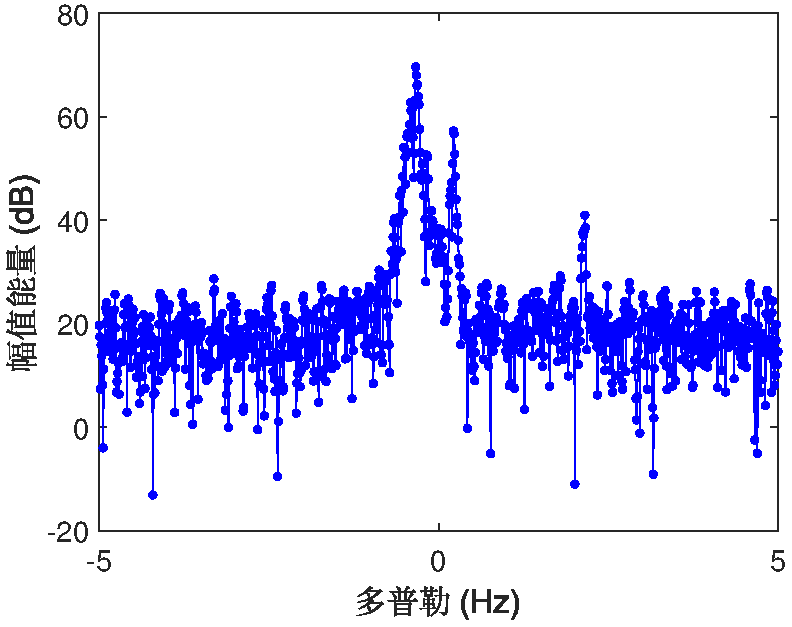
\includegraphics[width=6.67cm]{figures/othr/tosea}}
	\caption{复杂环境下频谱图}
	\label{fig:classical_spectrum}
\end{figure}


\subsection{数据集分组}
在本章的问题中,当雷达配置发生变化时,我们会获得不同的频率范围和精度频谱数据。例如,一些频谱数据的频率变化范围为-5Hz到5Hz、具有512个相干积累点,而另一些数据的频率变化范围为-10Hz到10Hz、相干积累点数为256个。因此,基于这两个条件,我们将所有数据分为4组:
\begin{itemize}
	\item 组 A: 如图\ref{fig:case128}所示,具有128个相干积累点数,频率变化范围为-5Hz到5Hz;
	\item 组 B: 如图\ref{fig:case256}所示,具有256个相干积累点数,频率变化范围为-5Hz到5Hz;
	\item 组 C: 如图\ref{fig:case512}所示,具有512个相干积累点数,频率变化范围为-5Hz到5Hz;
	\item 组 D: 如图\ref{fig:case1024}所示,具有1024个相干积累点数,频率变化范围为-5Hz到5Hz;
\end{itemize}
我们只选择了上述四个具有典型意义的分组的数据来进行验证,舍弃了其余类型的与他们相似的数据,例如频率变化范围为-10Hz到10Hz的具有512个相干积累点的数据,这与组B的数据基本相同。
\begin{figure}[H]
	\centering
	\subfloat[组 A]{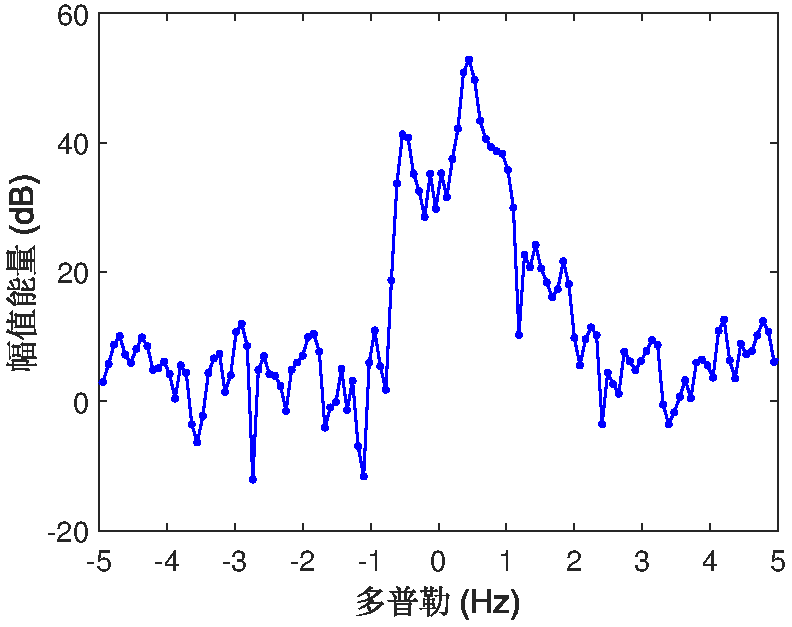
\includegraphics[width=6.67cm]{figures/othr/group128}%
		\label{fig:case128}}
	\hfil
	\subfloat[组 B]{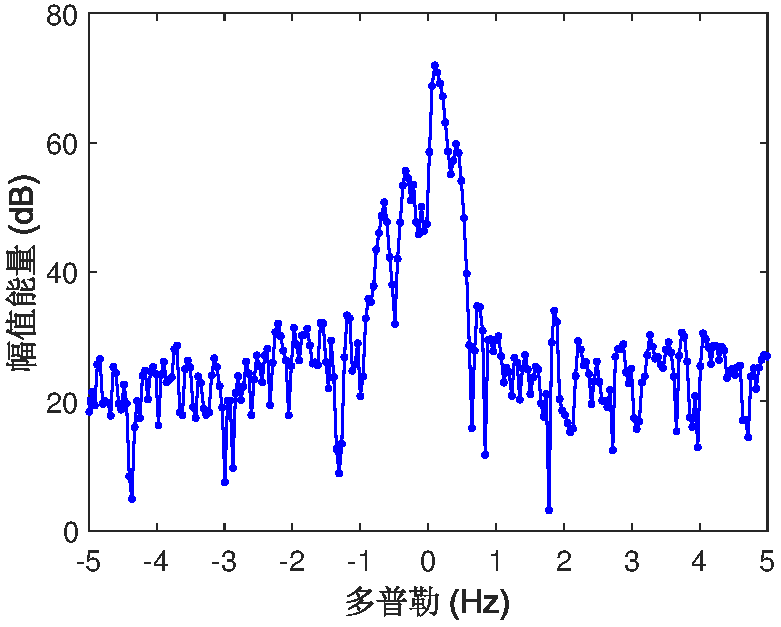
\includegraphics[width=6.67cm]{figures/othr/group256}%
		\label{fig:case256}}

	\subfloat[组 C]{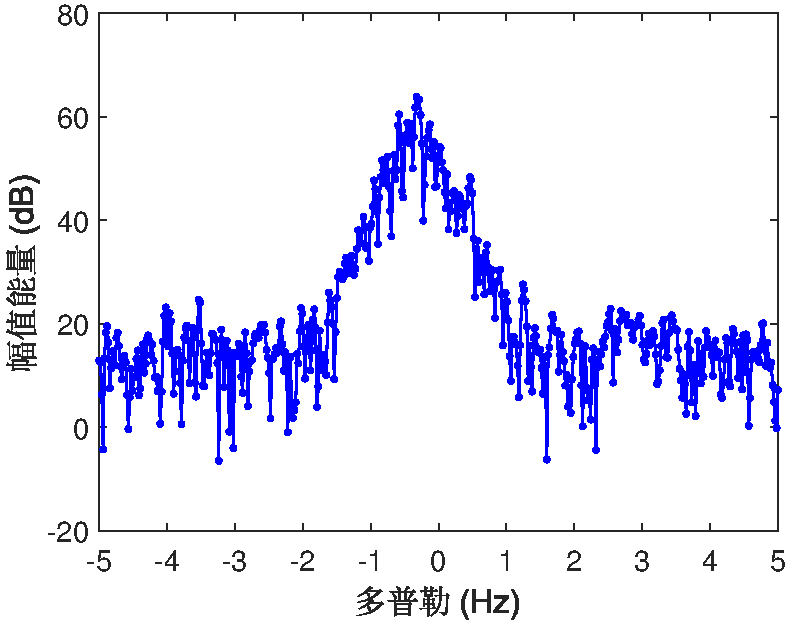
\includegraphics[width=6.67cm]{figures/othr/group512}%
		\label{fig:case512}}
	\hfil
	\subfloat[组 D]{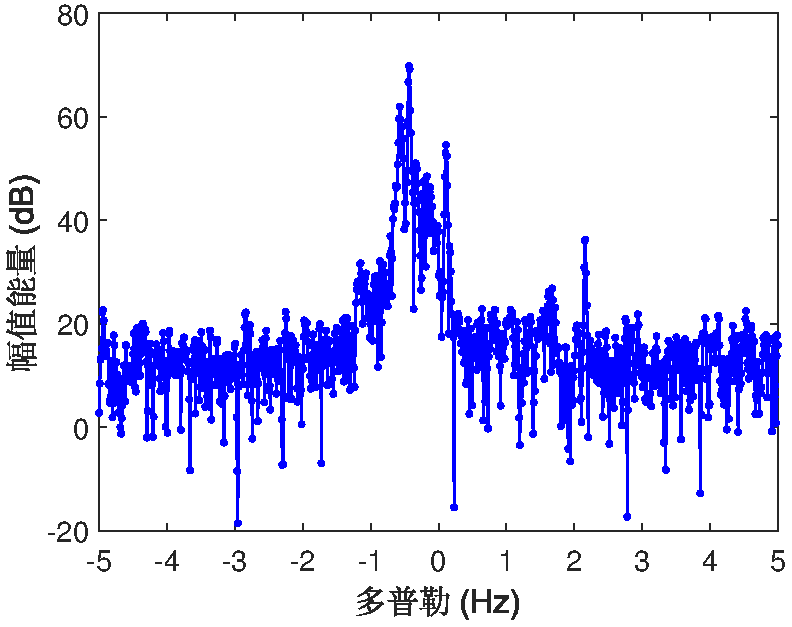
\includegraphics[width=6.67cm]{figures/othr/group1024}%
		\label{fig:case1024}}
	\caption{不同组数据的频谱对比示意图}
	\label{fig:group}
\end{figure}

\section{地海杂波识别算法}
天波超视距雷达目标的坐标配准问题在很大程度上影响了其定位精度,特别是对于电离层参数无法准确及时获得的较远。识别地海分界线主要有两个优点:第一个是我们可以使用获取的杂波地形图与实际的地图进行匹配,然后根据匹配结果计算偏移量,得到坐标修正系数,用来提高目标定位精度;另一方面,我们可以利用由识别结果获得的频谱上的偏移来校正频谱本身,以提高目标检测概率和准确度。

天波超视距雷达地海杂波识别技术的处理流程可分为信息预处理、地海杂波识别两个处理层,如图\ref{fig:system}所示。具体过程为:对频谱数据进行清洗、裁剪、融合等预处理操作,将预处理过的整体频谱数据输入到已经训练好的深度卷积神经网络分类器中进行识别。

\begin{figure}[H]
	\centering
	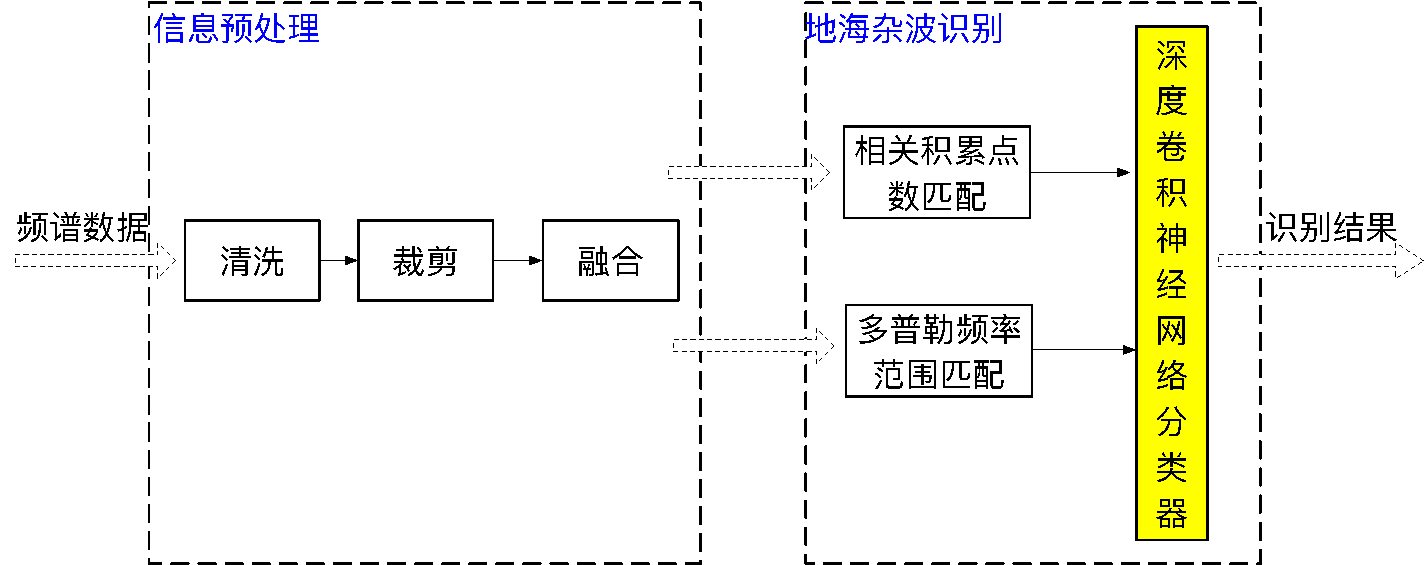
\includegraphics[width=13.5cm]{figures/othr/system}
	\caption{系统结构图}
	\label{fig:system}
\end{figure}

\subsection{数据预处理}
% 在本节中,我们首先介绍我们的算法的输入和输出变量。
% \subsection{特征向量和识别结果}
传统的分类问题一般利用各种不同的由原始数据进行变换得到的特征进行分类,本章利用原始的杂波频谱数据来做地海杂波的识别。同时针对于地海杂波识别问题的数据形式,本章对输入数据做了二次处理。
本章并没有选择某距离方位角单元的完整杂波频谱数据作为输入特征,而是考虑到用来区分地海杂波属性的特征主要集中于零频附近,因此对原始频谱数据做了剪切处理,只选择了零频附近一个区域的数据。通过减少大量无用数据,在一定程度上减少了计算量而且有助于防止过拟合现象的出现。

另一方面,我们最初从雷达得到的数据为对时域数据进行快速傅立叶变换后获得的频域中的数据,我们对这些数据进行平移,将快速傅立叶变换的直流分量移到频谱中心。虽然,表面上看利用平移前后的数据进行训练和测试区别不大。然而,在实际的情况中,在经过平移变换后,频域数据的特征更加集中,这样在执行卷积运算时学习得到的特征也更加准确。

\begin{figure}[H]
	\centering
	\subfloat[原始频率能量曲线]{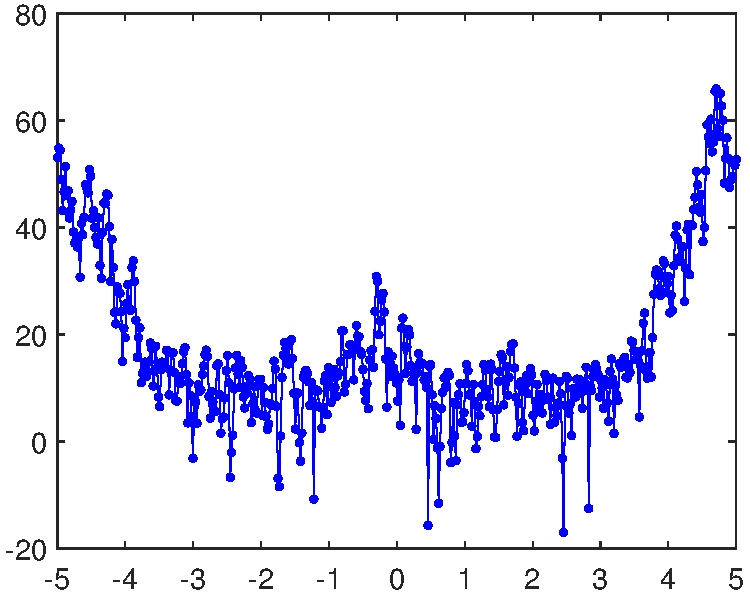
\includegraphics[width=6.67cm]{figures/othr/before_fft}%
		\label{fig:before_fft}}
	\hfil
	\subfloat[经过频率平移的频率能量曲线]{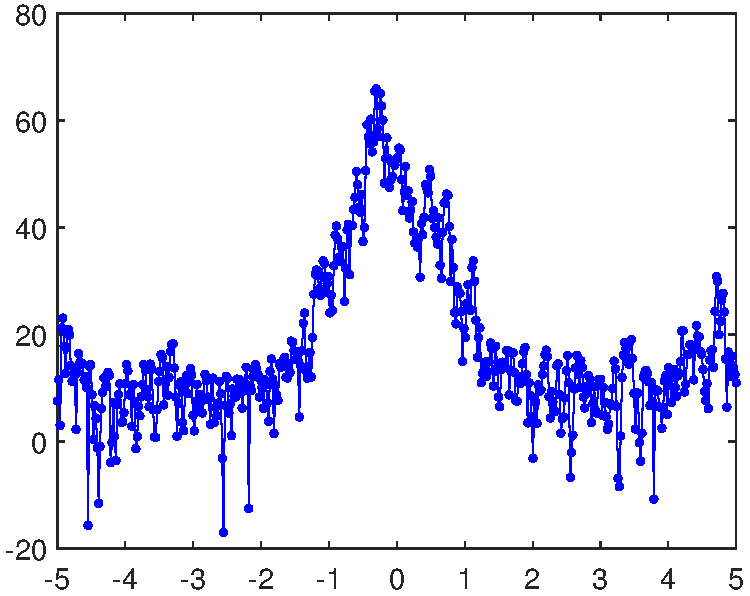
\includegraphics[width=6.67cm]{figures/othr/after_fft}%
		\label{fig:after_fft}}

	\caption{频谱数据平移变换示意图}
	\label{fig:fft}
\end{figure}

频谱数据预处理频谱数据是从天波超视距雷达获取的多普勒频率与幅度值对应的数据。在利用数据之前,我们首先对该数据进行清洗,把图\ref{fig:delete}这种并非处于正常探测模式下的数据进行去除。

由于数据来自不同波位、不同时刻,具有不同的雷达工作频率,我们在利用这些数据进行训练或者识别前需要首先对其进行基本的处理。主要包括将数据按照积累点数、波位和多普勒频率范围进行分类,不同类别的数据分开处理。另一方面,由于地海杂波特征主要集中于多普勒频率较低的区域,我们可以将数据进行裁剪,只选取有效数据(本章中在权衡信息保留以及计算量的清洗下,保留了处于零频附近,且频率范围为$[-5\text{Hz},+5\text{Hz}]$的区域),在一定程度上减小计算量。

\begin{figure}[H]
	\centering
	\begin{minipage}{7cm}
		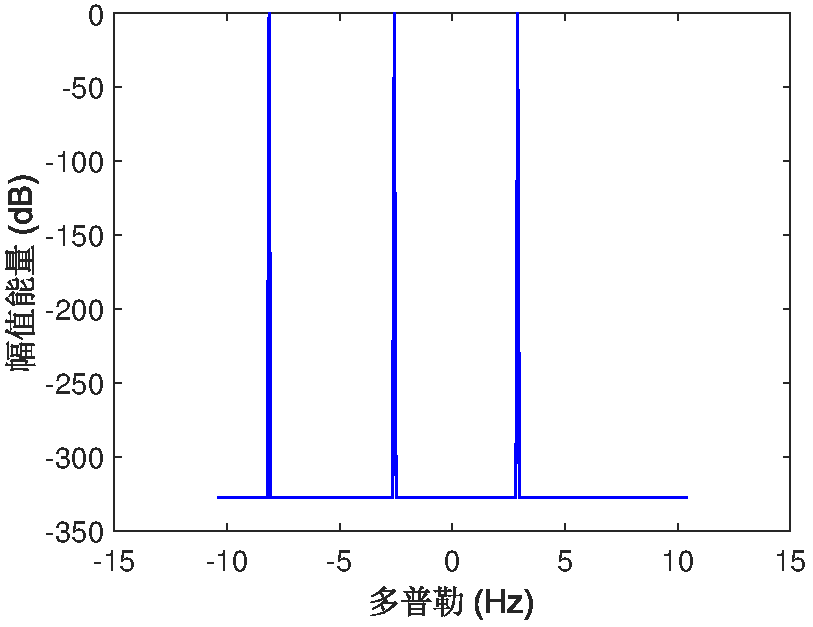
\includegraphics[width=6.67cm]{figures/othr/delete}
		\caption{需要被清洗掉的数据}
		\label{fig:delete}

	\end{minipage}
	\hspace{10pt}
	\begin{minipage}{7cm}
		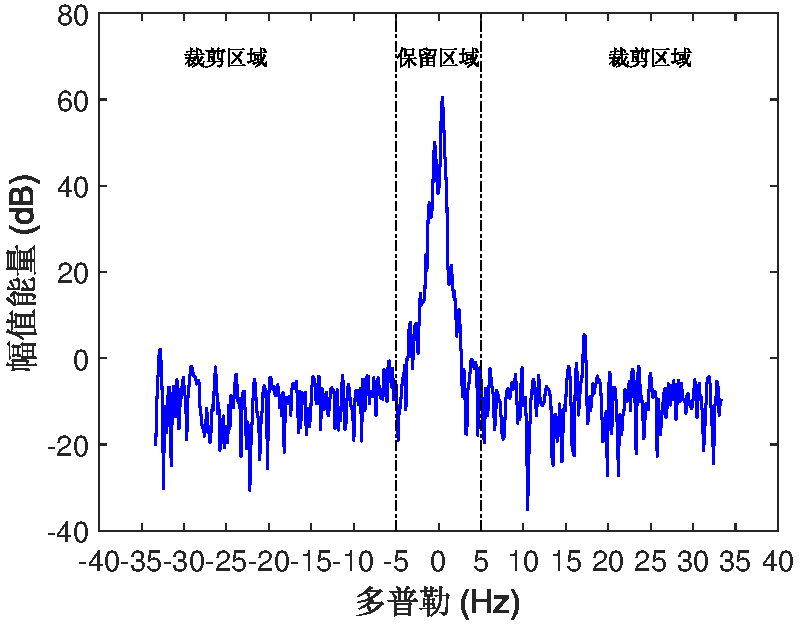
\includegraphics[width=6.67cm]{figures/othr/cut}
		\caption{数据裁剪示意图}
		\label{fig:cut}

	\end{minipage}

\end{figure}

受电离层非平稳、时变等特性影响,天波超视距雷达杂波数据可能会出现较大波动。对这种波动不加处理会导致地海杂波识别结果不准确。在一个相对短时间内,电离层会保持一个较平稳的状态,也即同一距离方位单元的真实的地海属性不会发生变化。因此,本章采用滑窗融合的方法对输入数据进行预处理。其基本思想是将连续窗长时间$N$ 内的相邻杂波数据$x_1,x_2,\dots,x_N$ 进行加权融合得到新的频谱数据作为深度卷积神经网络分类器的输入
\begin{equation}
	x=\sum_{i=1}^N w_ix_i
	\label{equ:window_fusion}
\end{equation}
其中$w_i$ 为频谱数据$x_i$ 的权重,关于窗长及权重的选择会在后面仿真验证小节进行详细的讨论。从图\ref{fig:spectrum_fusion}可以看出,融合后的毛刺明显变少,更利于最终的分类识别。

\begin{figure}[H]
	\centering
	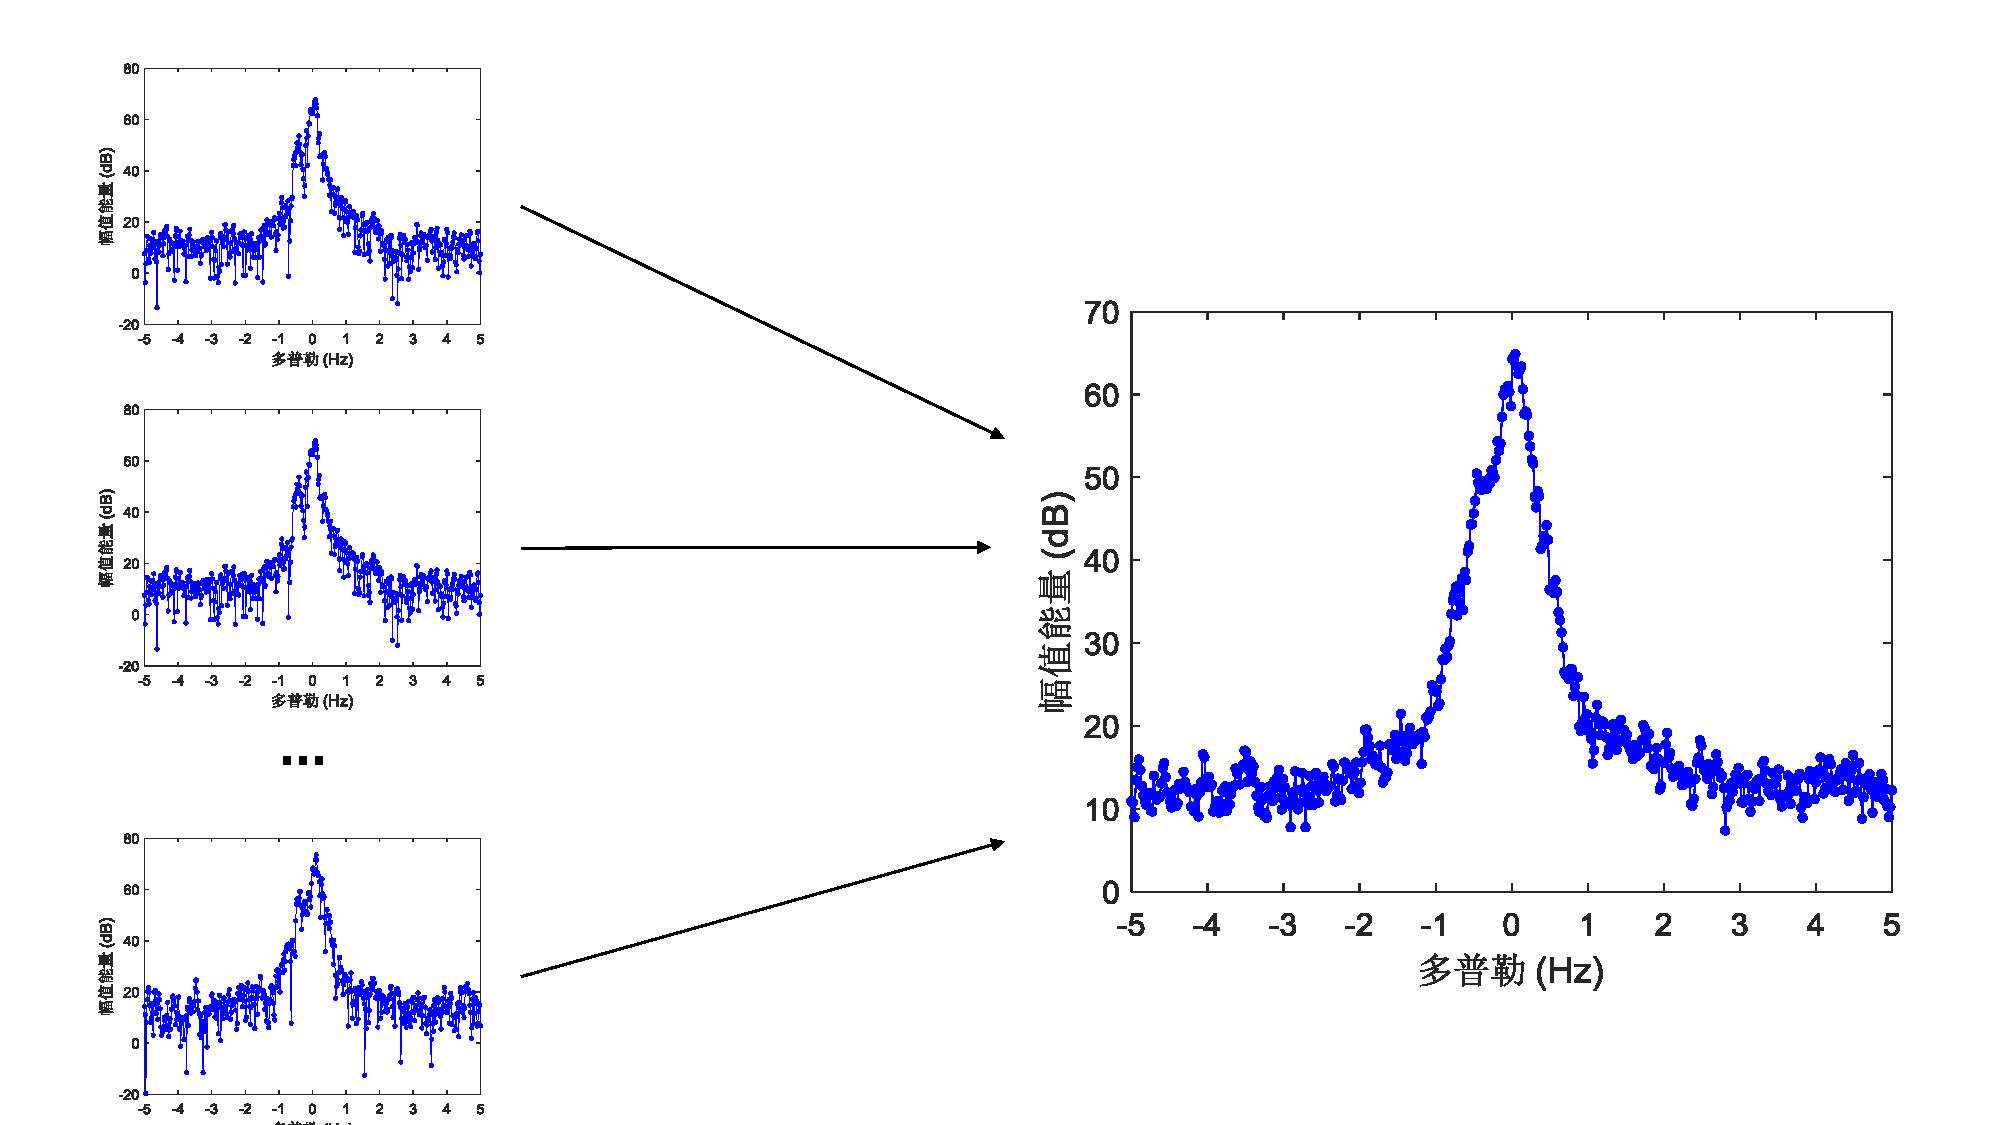
\includegraphics[width=13.5cm]{figures/othr/spectrum_fusion}
	\caption{数据融合示意图}
	\label{fig:spectrum_fusion}
\end{figure}

\subsection{分类算法设计}
深度学习体系结构中有几大网络模型,其中的卷积神经网络可以直接将整个需要分类的数据作为网络的输入,避免了传统识别算法中复杂的特征提取和数据重建过程。基于此优点,使卷积神经网络在本章所需解决的天波超视距雷达地海杂波特征识别问题中有着巨大优势。
本章利用深度学习中的深度卷积神经网络算法,避免了对于地海杂波的建模,也即从根本上避免了传统方法所面对的困难。如图 \ref{fig:othr_tech} 所示,其主要可分为训练和识别两个步骤:利用大量已打好标签的样本通过深度卷积神经网络进行训练;然后对于新得到的雷达频谱数据利用模型进行识别,获得当前频谱数据的识别结果。

\begin{figure}[hbt]
	\centering
	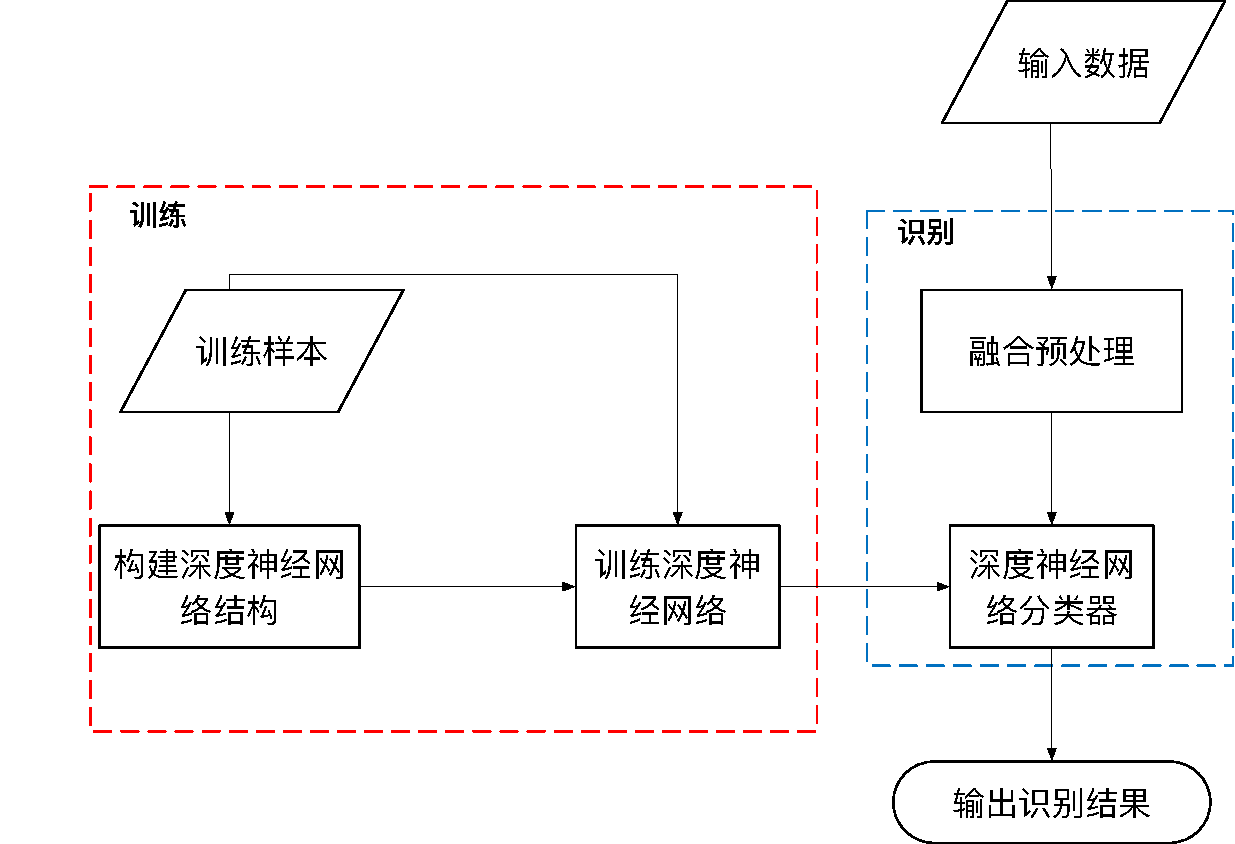
\includegraphics[width=9cm]{figures/othr/othr_tech}
	\caption{地海杂波识别技术结构图}
	\label{fig:othr_tech}
\end{figure}

利用深度卷积神经网络进行天波超视距雷达地海杂波识别过程的主要挑战与难点在于网络模型的设计。典型的卷积神经网络由深层结构堆叠在一起的多个不同的层组成:输入层,多组卷积和池化层,有限数量的完全连接的隐层,以及输出层。
如图\ref{fig:fullconnect}所示,本章设计的深度卷积神经网络的结构在功能上可以分为特征提取和全连接网络这两部分,特征提取层主要通过卷积操作和池化操作从输入的频谱数据中学习出最好的卷积核以及这些卷积核的组合方式,同时每一层的输出又作为下一层的输入,每层具有多个特征向量,每个特征向量具有多个神经元,并且每个特征向量来自于一种卷积核所提取输入的一种特征;全连接网络,主要是将任何一个神经元均和上一层的任何神经元之间建立管理,通过矩阵运算得到输出结果。
\begin{figure}[hbt]
	\centering
	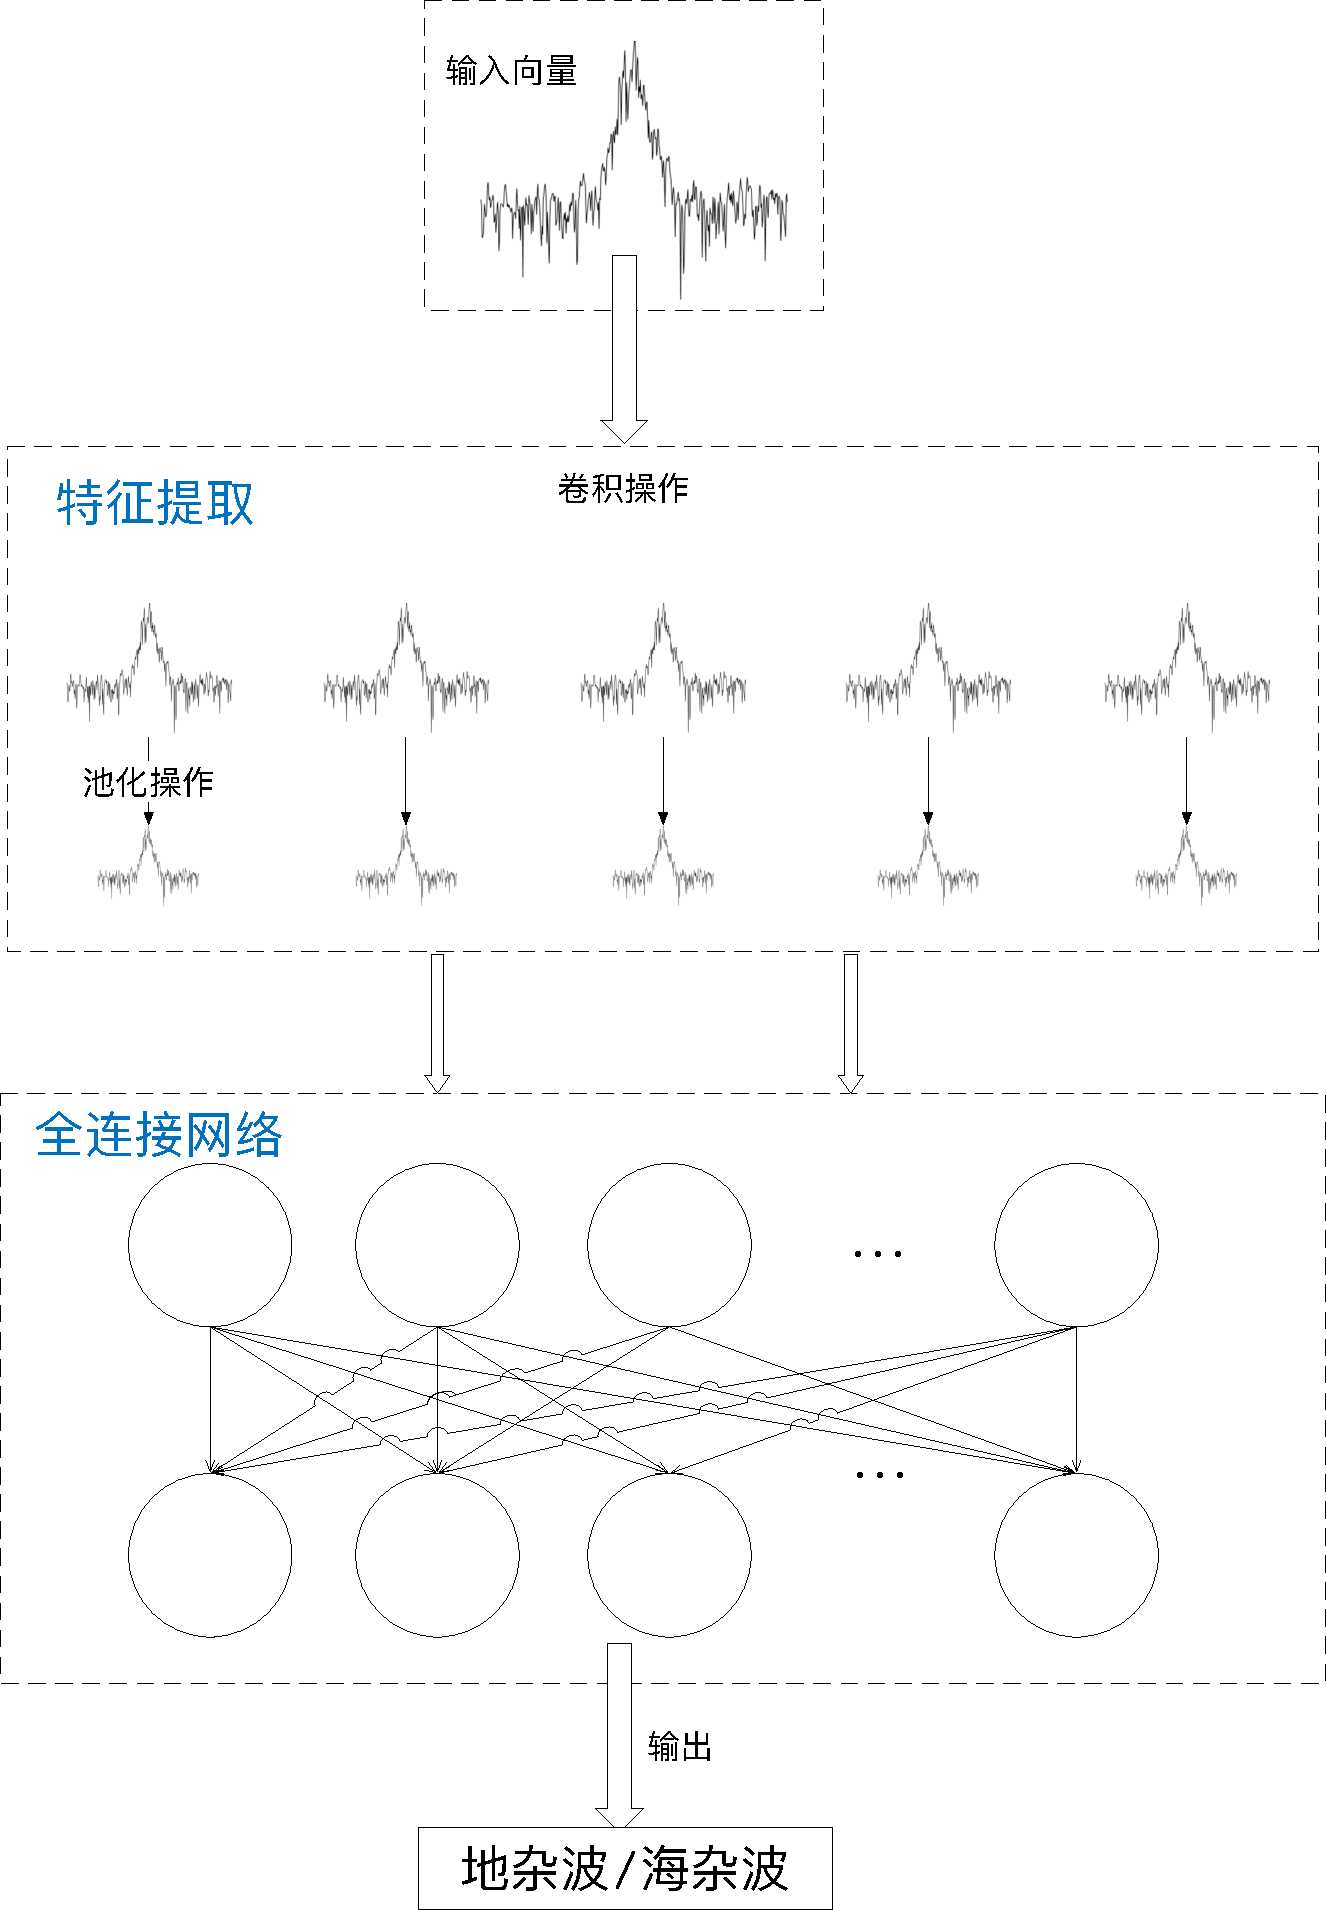
\includegraphics[width=6.67cm]{figures/othr/fullconnect}
	\caption{特征提取和全连接网络}
	\label{fig:fullconnect}
\end{figure}

我们的地海杂波识别问题主要是基于频谱数据的特征来识别。人工识别主要基于海杂波中存在关于零频对称的Bragg峰,而地杂波只存在零频率附近的一个峰值。然而,还有一些无法直观的描述的特征,如整体幅度等等。此外,在一些频谱数据中仍然有一些无用的特征,例如,出现一个目标,这部分可以通过卷积特征提取和权重共享容易地去除对最终识别的影响。因此,本章基于CNN的方法很适合我们的问题。

通过利用CNN进行地海杂波识别,避免了对天波雷达回波的建模,从根本上避免了传统方法所面临的困难。本章根据地海杂波频谱的实际数据以及其反映出来的特性,构建了一个具有六层的基本卷积神经网络,如图\ref{fig:struct}所示,每层具有多个特征向量,每个特征向量具有多个神经元,\textcolor{red}{并且每个特征向量从提取输入的卷积滤波器的特征导出}。构建神经网络结构的其基本步骤为:

步骤1:输入地海杂波频谱数据(此处以大小为$1\times N$ 的输入序列为例),对其进行卷积运算,得到第一个卷积层。本章经过不同参数的试验对比结果,最终确定使用32个大小为$1\times 3$ 的卷积核,故特征向量中每个神经元与输入中的$1\times 3$ 的邻域相连,这样此卷积层中的特征大小就为$1\times (N-3)$ 。又因为该卷积层有128个可训练参数(每个滤波器具有3个单元参数和一个偏置参数,一共32个滤波器,共$(1\times 3 + 1) = 128$ 个参数),共$128\times(N-3)$ 个连接,将连接通过ReLU激活函数。

步骤2:对卷积层进行最大池化处理,该操作将相邻的多个特征采用一个特征进行代替。通过降低特征向量的长度,在减小了计算量的同时也在一定程度上修正了过拟合情形。

步骤3:将经过上述两个步骤获得的特征向量作为新的输入,重复三次步骤1至2,可以得到一个三阶段的深度卷积神经网络结构。通过上述多阶段卷积操作,输入向量的特征获得了充分的提取。

步骤4:构建输出层。压平步骤3获得的特征向量,把多维的输入一维化,以此作为卷积层到全连接层的一个过渡。在第一个全连接层的基础上添加dropout 参数,然后添加第二层全连接并通过激活函数Sigmoid ,输出识别结果。

\begin{figure}[hbt]
	\centering
	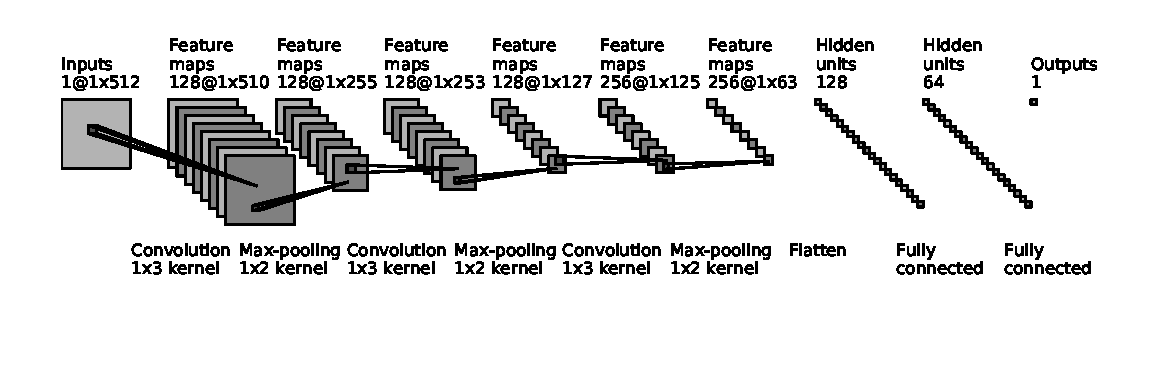
\includegraphics[width=13.5cm]{figures/othr/struct}
	\caption{卷积神经网络结构}
	\label{fig:struct}
\end{figure}

\subsubsection{训练算法}

深度神经网络训练过程在搭建好合理的深度神经网络结构之后,下一步需要利用大量的数据对该网络进行训练。对于本章数据的训练的基本流程,对于地海杂波识别问题由于需要对不同相干积累点数和多普勒频率范围的数据进行分开训练,故首先需要对不同的数据进行分类处理并标注其地海杂波类型,通过此步骤完成训练样本的生成。接下来就是利用训练样本对搭建好的网络结构进行训练,获得最终的分类器。训练过程或者说学习过程主要是利用了梯度下降算法,梯度反映了参数的移动方向。这其中一个很重要的问题就是学习率的选择,学习率过小则运行缓慢,过大则无法得到很好的结果。

传统的神经网络优化方法是mini-batch梯度下降。这个想法是计算每次迭代的mini-batch梯度,然后更新参数。然而,这种方法有两个缺点,一个是学习率的选择比较困难,因为它对所有参数使用相同的学习率,故很难选择一个很合适的初值,另一个是趋向于收敛到局部最优。

\textcolor{red}{
本章不仅考虑梯度,同时考虑包含梯度变化的信息,采用了一种具有自适应学习率的优化算法Adam(Adaptive Moment Estimation)。该算法利用梯度的一阶矩估计和二阶矩估计动态地调整每个参数的学习率。经过偏置校正后,每一次迭代学习率都有明确范围,使得参数更加平稳。
传统的梯度下降更新规则为$\theta \rightarrow \theta'=\theta-\eta\nabla C$ ,这里$\theta$ 表示需要学习的参数,$\eta$ 为学习速率,$\nabla C$ 为损失函数的梯度,则变为:
\begin{align}
	v\leftarrow v'=\mu v - \eta \nabla C \\
	\theta \leftarrow \theta' = \theta +v'
\end{align}
其中,$\mu$ 是用来控制梯度变化的超参数。
}
训练神经网络模型。在搭建好神经网络模型后,利用训练样本对该模型做进一步训练,其基本的算法流程如下:

\begin{algorithm}[hbt]
	\caption{Adam 训练算法}
	\begin{algorithmic}[1] %每行显示行号
		\Require 训练样本$X$,样本标签$Y$,最大迭代次数$K$,步长$\varepsilon$,初始目标参数$\theta$
		\Ensure 学习后的参数$\theta$
		\State 初始化矩估计的期望衰变率$\rho_1=0.9,\rho_2=0.999$,一阶矩与二阶矩变量$s=0,r=0$,迭代次数$k=0$
		\While{$k < K$}
			\State 从训练集中获取对应于目标$y^{(i)}$ 的$m$ 个采样样本 $\{x^{(1),\dots,x^{(m)}}\}$ ,其中$m$ 为批处理中一批样本的个数。
			\label{line:start}
			\State 计算梯度$g \leftarrow \frac{1}{m} \nabla_{\theta} \sum_i L(f(x^{(i)};\theta), y^{(i)}) $,其中$L$为对数损失函数,其定义为$L(P(Y|X),Y) = - \log P(Y|X) $。
			\State 更新迭代次数$k \leftarrow k+1 $
			\State 更新有偏一阶矩估计$s \leftarrow \rho_1 s + (1 - \rho_1) g $,有偏二阶矩估计$r \leftarrow \rho_2 r + (1-\rho_2) g \odot g $,其中$ g \odot g $表示对应元素的乘积。
			\State 修正一阶矩估计$\hat{s} \leftarrow \frac{s}{1-\rho^k_1} $,二阶矩估计$\hat{r} \leftarrow \frac{r}{1-\rho^k_2} $。
			\State 更新参数 $\theta \leftarrow \theta + \Delta \theta = \theta - \varepsilon \frac{\hat{s}}{\sqrt{\hat{r}} + \delta} $
			,其中$\delta = 10^{-8} $
			用来保持稳定性。
		\EndWhile
	\end{algorithmic}
\end{algorithm}

由于本章是一个二分类的问题,我们利用逻辑损失函数来训练本章的模型。
\begin{equation}
	L(z_i) = log(1+e^{-z_i})
\end{equation}
其中, $z_i=y_i(w^T x_i + b)$, $y_i$ 是采样样本 $x_i$的标签,其为1代表地杂波,0为海杂波。

\subsection{分类阈值设计}
由于我们的问题是一个二分类问题,所以我们得到的是回波频谱数据是来自于海洋还是陆地的概率。对于一般的二分类问题,我们可以使用$ 0.5 $作为概率阈值来进行分类。但是,在我们的问题上,结合实际的情况,我们需要考虑下面两个方面:
\begin{itemize}
	\item 海洋的变化远远大于陆地,海洋容易被误判为陆地。
	\item 海洋或者陆地均应该是连续的。
\end{itemize}
因此,我们不能直接输出结果。我们需要找到合适的阈值来划分地海杂波,这将在第\ref{section:experiment}节通过仿真实验进行讨论。
此外,我们还需要根据该距离方位单元周围单元的识别结果进行进一步处理。也就是说,如果我们得到初步结果$y_{i,j}$,$i$表示方位角的第$ i $ 个单元,$ j $表示第$ j $个径向距单元。那么,最终结果$y_{i, j}$可以表示为:
\begin{equation}
y_{i, j} = \sum_{m=1}^{M}\sum_{n=1}^{N}w_{m,n}\cdot y_{m,n}
\end{equation}
$ w_{m,n} $是$(m,n)$单元处识别结果$y_{m,n}$的权重,$M$为利用的方位上的区域单元个数,$N$为利用的径向距上的区域单元个数。
\section{仿真验证}
在本节中,我们利用实际数据评估了我们提出的基于深度学习的地海杂波识别算法的性能。将我们的基于CNN的算法与基于LMS\ucite{turley2013high}的根据多普勒频谱进行分类的算法和基于支持向量机进行分类的算法\ucite{jin2012svm}进行了对比,我们算法相对于其余两种算法在性能上的提高,证明了我们算法的可用性。
\subsection{算法实现}
\subsubsection{基于LMS的算法}
该方法主要基于文献\cite{turley2013high},其基本思想是利用加权最小均方算法来求解区域的模糊度,其中区域模糊度的定义如下:
\begin{equation}
	f_D = f_I + f_{cur} + f_B\left\{
		\begin{array}{rcl}
		1/2       &      & \text{前向海}\\
		0     &      & \text{陆地}\\
		-1/2       &      & \text{后向海}
		\end{array} \right.
\end{equation}
其中, $f_B$ 是前向Bragg回波与后向之差,$f_I$ 和 $f_{cur}$分别是电离层动力过程和海流产生的多普勒频偏。

% 首先介绍一种常用于工程实践中的地海杂波识别算法,单阈值法。通常,海洋和陆地杂波的差异在于,地杂波最大能量的频率几乎为零。然而,海杂波存在沿着零频率对称的有两个类似的峰,称为布拉格峰。因此,我们可以使用频率$ f $来判别频谱数据的地海杂波属性。
% \begin{equation}
% f_{i, j}= \mathop{\arg\max}_{f} \ \ x(i, j, f)
% \end{equation}
% $x(i, j, f)$ 是在频率 $f_{i, j}$下的能量值。在已知 $f_{i, j}$ 的情况下, 我们需要和阈值 $\eta$ 比较来判断其地海属性。
% \begin{equation}
% 	y_{i, j}= \left\{\begin{array}{ll}
% 		0&|f_{i, j}| > \eta, \\
% 		1&|f_{i, j}| < \eta
% 		\end{array}
% 		\right.
% \end{equation}
% 0代表海洋,1代表陆地。
\subsubsection{基于SVM的方法}
这里我们参照文献\cite{jin2012svm},选择了如下三个特征作为分类器的特征向量:
\begin{itemize}
	\item 最大后向散射幅值
	\item 频谱中最大与次大幅值频率之差
	\item 频谱中最大与次大幅值幅度之差
\end{itemize}
同时,我们利用了网格法对参数进行了调优。

为了确保我们有足够的数据来训练和测试我们的算法,我们选取了不同的雷达工作条件、天气、时间的多组数据(每组约有20000个频谱数据)。我们随机选择其中$70\%$的数据作为训练数据,$20\%$作为交叉验证数据,其他数据用作测试数据。

\subsubsection{我们的算法}
我们根据图 \ref{fig:struct} 所示的结构搭建了本章的深度卷积神经网络分类器。对于前两个卷积层具有32个滤波器,对于第三个卷积层有64个滤波器。全连接层添加到dropout参数为0.5 。利用Adam优化算法来训练网络,初始的学习率为0.001,基本迭代次数为20次。我们使用相同的样本来分别训练和测试基于支持向量机的分类器和我们的算法。

\subsubsection{评估方法}
对于一个分类问题,最基本的算法性能评估方法是分类的准确度。然而,由于我们这里利用实际数据进行验证,这些数据没有准确的标签,尤其是地海交界处的杂波的类别更加难以确定。而在实际工程实践中,该部分的识别准确度影响着最终电离层参数的辨识。由于在实际的地图中可以得到地海交界处也即海岸线处的地理位置坐标,也即可以得到该区域的形状。因此,我们设计了与地图的匹配程度的评估方法来分析不同识别算法对于海岸线部分杂波识别的性能,其基本定义如下:
\begin{equation}
g_{C_1, C_2} = \frac{area({C_1\cap C_2})}{\max(area({C_1}), area({C_2}))}
\end{equation}
我们用0和1来二值化我们的区域,如图\ref{fig:binary}所示。$area(C)$表示区域$C$的面积, $g_{C_1, C_2}$表示区域$C_1$ 和 $C_2$ 的匹配度。
\begin{figure}[hbt]
	\centering
	
\includegraphics[width=6.67cm]{figures/othr/binary}
	\caption{二值化地图}
	\label{fig:binary}
\end{figure}

\subsection{仿真结果分析}
\label{section:experiment}
% 在此基础上,我们使用相同的样本来分别训练和测试基于支持向量机的分类器和我们的算法。实验结果表明我们的算法具有更好的稳定性和准确性。
我们首先利用我们的四组数据对于三种算法进行了对比分析。实验结果如表\ref{tab:methods}所示,可以明显的看到,我们的算法的识别正确率为最优。
\begin{table}[H]
	\renewcommand{\arraystretch}{1.3}
	\caption{三种算法的识别精度对比}
	\label{tab:methods}
	\centering\sWuhao
	\begin{tabularx}{\textwidth}{>{\centering\arraybackslash}X>{\centering\arraybackslash}X>{\centering\arraybackslash}X>{\centering\arraybackslash}X}
		\toprule
		数据集 & CNN & SVM & LMS \\
		\midrule
		组 A  & 96.97\% & 85.69\% & 81.85\% \\
		组 B & 97.14\% & 88.57\% & 81.93\% \\
		组 C & 99.04\% & 89.03\% & 88.57\% \\
		组 D  & 99.69\% & 91.61\% & 90.33\% \\
		\bottomrule
	\end{tabularx}
\end{table}
我们选取了CNN部分识别错误的结果进行分析,如图 \ref{fig:error_result} 所示,发现该部分的数据属于特征十分不明显的内容,即使是人工判定也无法很准确的判定的结果。

\begin{figure}[H]
	\centering
	\subfloat[地杂波被错误识别为海杂波]{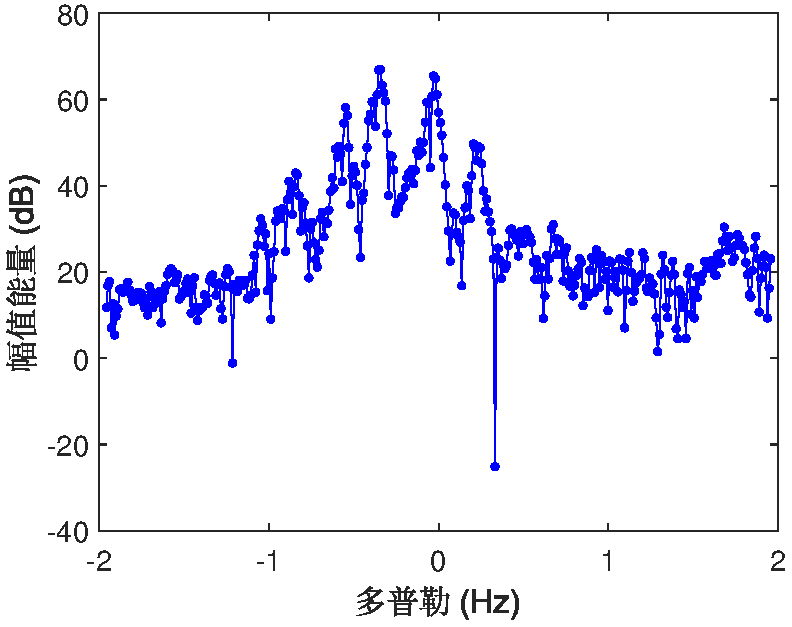
\includegraphics[width=6.67cm]{figures/othr/error_land}%
		\label{fig:error_land}}
	\hfil
	\subfloat[海杂波被错误识别为地杂波]{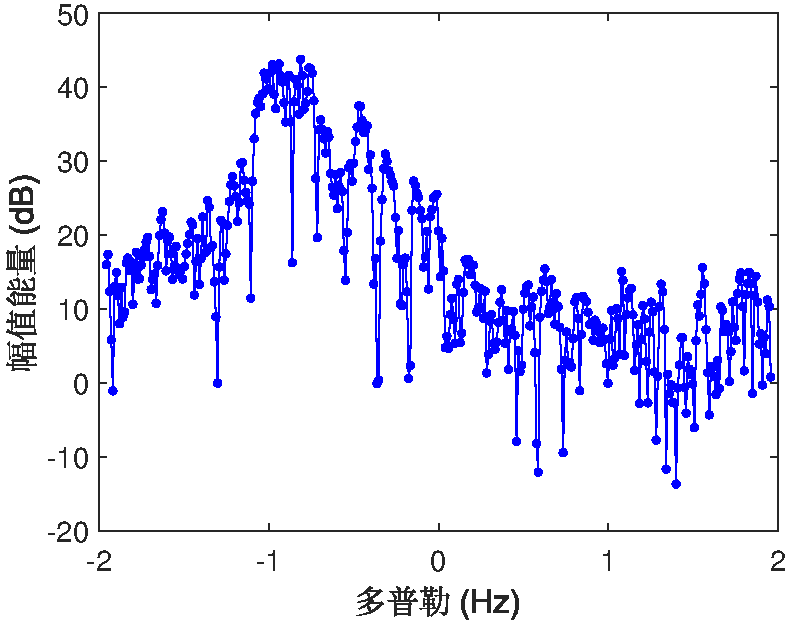
\includegraphics[width=6.67cm]{figures/othr/error_sea}%
		\label{fig:error_sea}}
	\caption{识别错误的结果}
	\label{fig:error_result}
\end{figure}

由于数据集自身的一些限制条件,我们选择在组D所在的数据集进行了地图匹配度的比较实验。从表\ref{tab:method_pair}可以看出,我们的算法在匹配度方面要远高于其余两种方法,证明了我们的算法在地海边界处仍然可以保持很高的精度。
\begin{table}[H]
	\renewcommand{\arraystretch}{1.3}
	\caption{匹配度对比}
	\label{tab:method_pair}
	\centering\sWuhao
	\begin{tabularx}{\textwidth}{>{\centering\arraybackslash}X>{\centering\arraybackslash}X>{\centering\arraybackslash}X>{\centering\arraybackslash}X}
		\toprule
		& CNN & SVM & LMS \\
		\midrule
		匹配度 & 0.92 & 0.23 & 0.21 \\
		\bottomrule
	\end{tabularx}
\end{table}

%TODO: \textcolor{red}{添加对于三个判断结果参数的设计}

为了验证我们的深度卷积网络在迭代次数方面的影响,其不同组数据的损失函数如图\ref{fig:group_results}所示,结果表明我们的算法可以在不同的数据集组中均可以较快的收敛。虽然,对于相同的神经网络结构,第一个数据集需要最多的迭代次数才能收敛,这是因为当频率和相干累计点的比例变小时信息或者说特征也随之减少,故需要较多的迭代次数。

图\ref{fig:sizes}展示的是在样本集大小不同的情况下,我们的算法与基准算法的平均分类准确率的对比图。由于基准方法仅使用根据先验知识得到的阈值,因此随数据集增长其识别准确度变化不大,而我们的深度卷积神经网络的算法随着数据集内样本数量的增加,准确度有着显著提升。

\begin{figure}[hbt]
	\centering
	\begin{minipage}{7cm}
		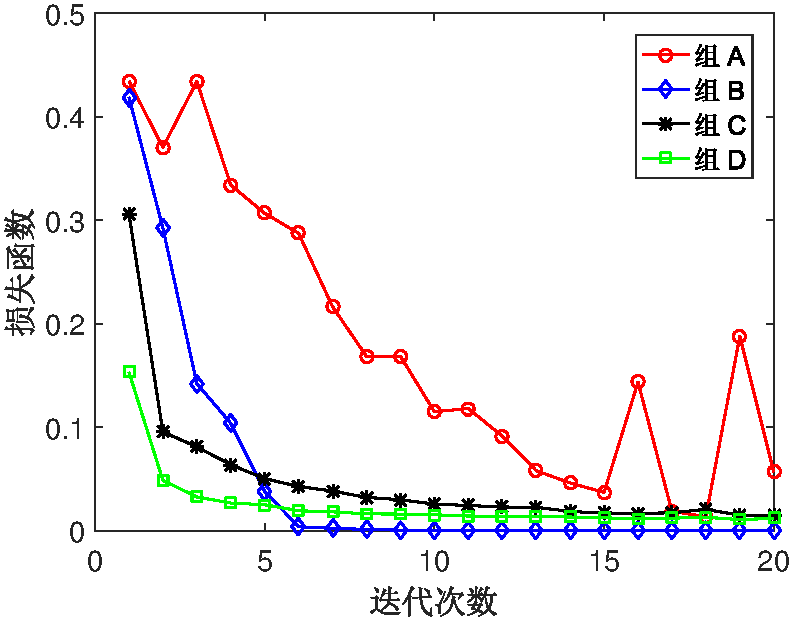
\includegraphics[width=6.67cm]{figures/othr/group_results}
		\caption{不同数据集损失函数对比图}
		\label{fig:group_results}
	\end{minipage}
	\hspace{10pt}
	\begin{minipage}{7cm}
		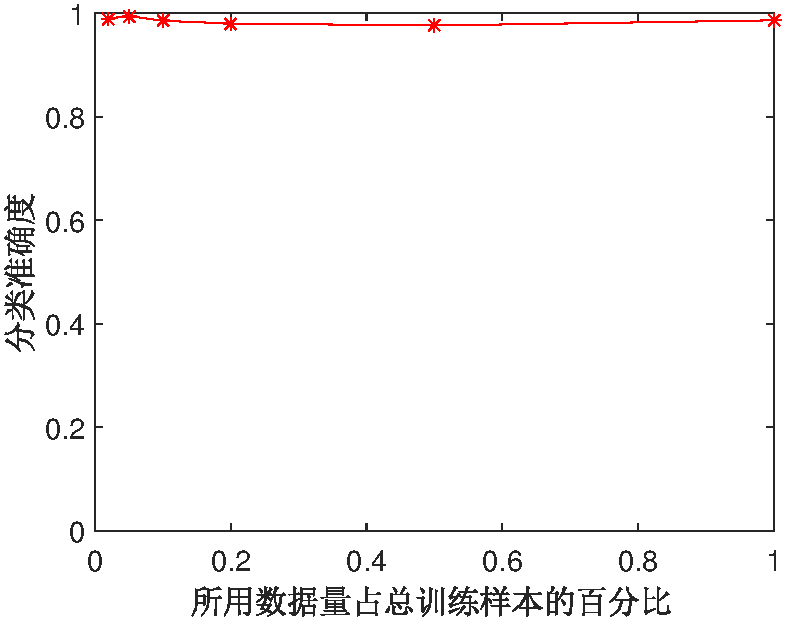
\includegraphics[width=6.67cm]{figures/othr/sizes}
		\caption{不同数量数据集的分类准确度对比曲线图}
		\label{fig:sizes}

	\end{minipage}

\end{figure}


众所周知,卷积神经网络的参数对于最终分类识别的准确率起着重要的作用。因此,我们需要对参数的选择进行一些分析。首先,我们分析在批长度(Batch Size)和迭代次数变化时,验证集数据的分类准确度。如图\ref{fig:epoch}所示,我们可以发现识别准确度随着迭代次数的增加而增长。而当批长度变大时,收敛速度加快。
\begin{figure}[H]
	\centering
	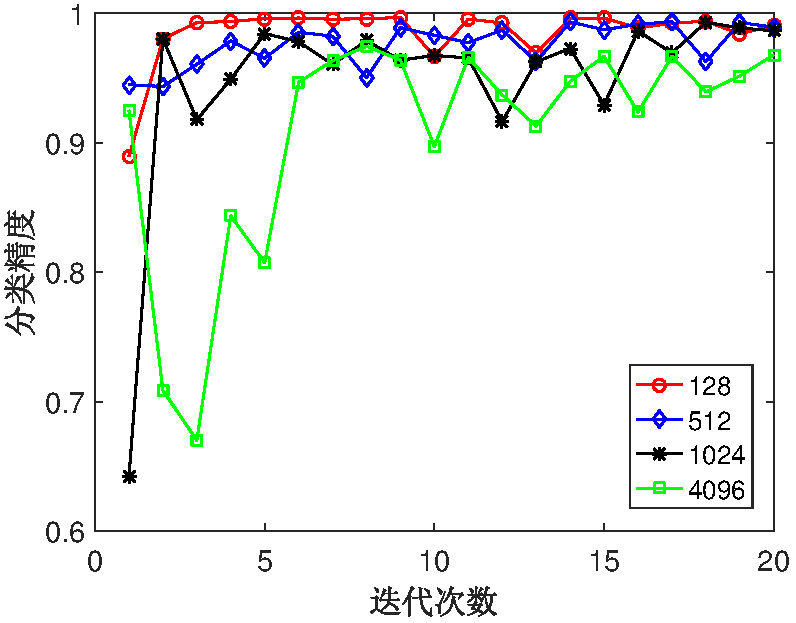
\includegraphics[width=6.67cm]{figures/othr/epoch}
	\caption{不同批长度下,分类准确度与迭代次数曲线图}
	\label{fig:epoch}
\end{figure}

由于在预处理阶段,本章利用了滑窗算法对输入数据进行融合处理来减少由于某一帧数据中某距离方位单元由于出现的随机噪声对于我们识别结果的影响,此处对窗长参数进行设计比较。本章主要考虑到电离层会随时间发生变化且天波雷达的采样周期较长,过长的窗长对无法及时的响应电离层的变化,影响识别准确率以及与地图的匹配度。
为了取得一个合适的窗长,我们首先利用不同窗长平均融合后的数据进行测试,得到图 \ref{fig:window} 的结果,该结果证明了在窗长过长时候,匹配度会下降的结论,当窗长过大时匹配度会降到比窗长为1时还要低。为了进一步比较权重的变化对于识别结果的影响,我们选取\equref{equ:window_fusion}中的权重为$w_N=\frac{1}{2},w_k=\frac{1}{2(N-1)},k=1,2,\dots,N-1$
,得到如图\ref{fig:weighted_window}所示的结果。由于增加了主单元的权重,故其可以在窗长增加时,不会有过于明显的匹配度下降。


\begin{figure}[H]
	\centering
	\begin{minipage}{7cm}
		\centering
		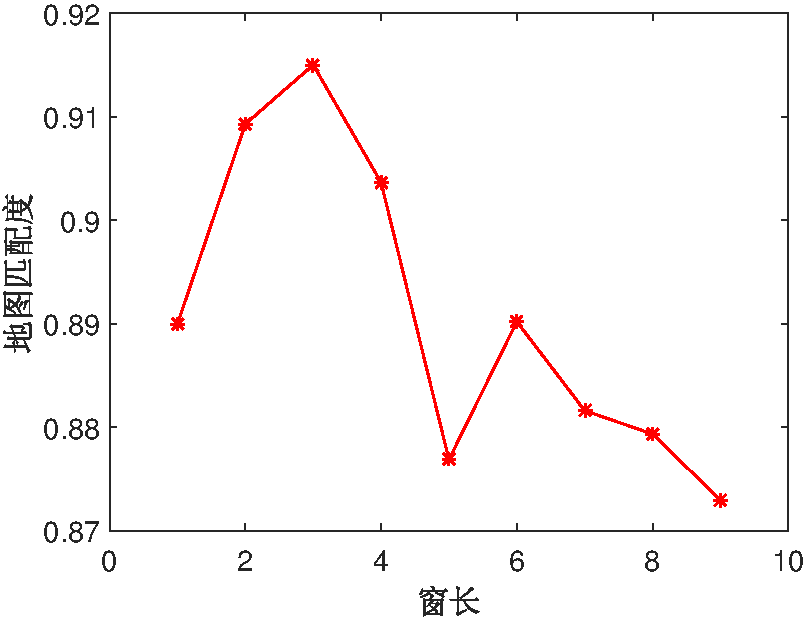
\includegraphics[width=6.67cm]{figures/othr/window}
		\caption{匹配度与融合窗长对比曲线图}
		\label{fig:window}
	\end{minipage}
	\hspace{10pt}
	\begin{minipage}{7cm}
		\centering
		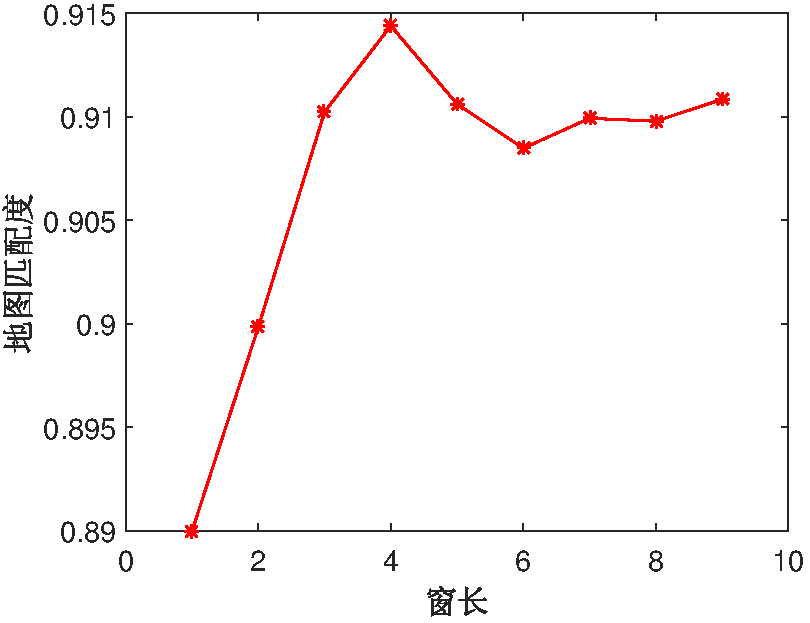
\includegraphics[width=6.67cm]{figures/othr/weighted_window}
		\caption{更改权重后不同窗长匹配度结果对比曲线图}
		\label{fig:weighted_window}
	\end{minipage}

\end{figure}


为了找出区分识别结果中海洋与陆地的最佳概率阈值,我们使用不同的概率阈值计算相同测试数据的正确率。图\ref{fig:threshold}显示,当阈值增大时,分类识别精度也随之提高,但精度的提高速度越来越慢,直至平稳。另一方面,当阈值仅为$0.01$时,识别率仍高于$0.86$。这说明我们的方法的分类结果的概率值均处于较高的水平,如\ref{fig:prob}所示。

\begin{figure}[H]
	\centering
	\begin{minipage}{7cm}
		\centering
		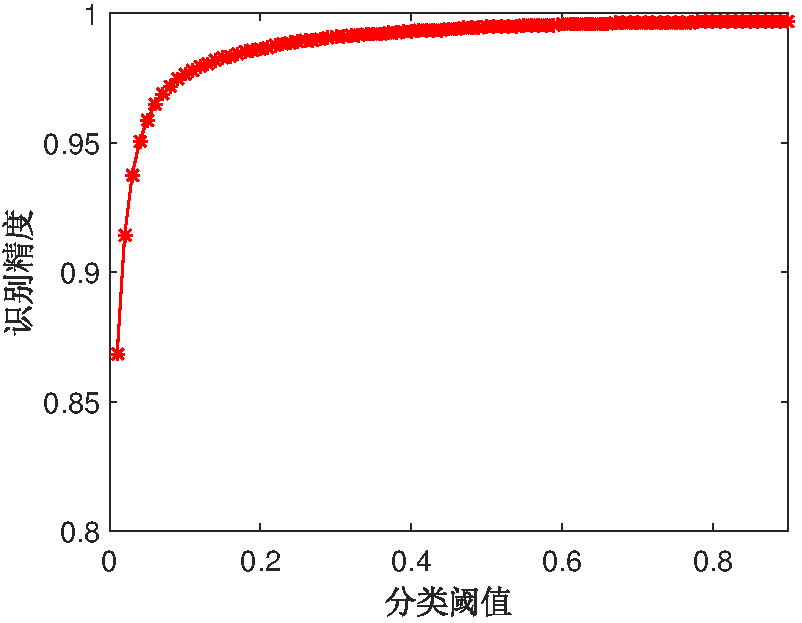
\includegraphics[width=6.67cm]{figures/othr/threashold}
		\caption{识别率与概率阈值曲线图}
		\label{fig:threshold}
	\end{minipage}
	\hspace{10pt}
	\begin{minipage}{7cm}
		\centering
		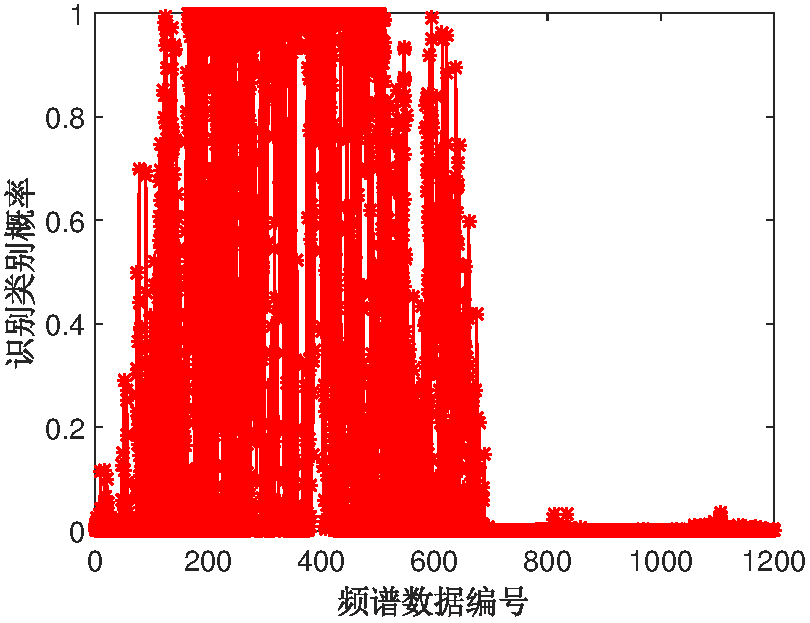
\includegraphics[width=6.67cm]{figures/othr/prob}
		\caption{不同帧数据识别结果概率值}
		\label{fig:prob}
	\end{minipage}

\end{figure}


为了验证本章提出的深度卷积神经网络地海杂波识别算法是否具有实时识别的能力,我们在CPU为i5-3.30GHz、运存为1GB的Linux虚拟机运行本章的算法程序,对整帧的实际雷达数据(共 20400 个分辨单元,每个分辨单元的相干积累点数为1024),其识别过程中占用内存峰值为178.5MB,识别时间为0.494141秒,其具备实时运行的能力。


经过上述实验在多个不同数据集上,对我们的算法和基于支持向量机的识别算法和基于LMS的算法的对比分析,可以得到下述结论:
\begin{itemize}
	\item 我们基于卷积神经网络的方法中获得最好的结果,且在地图匹配结果方面显著优于其余两种方法。
	\item 我们的方法具有很强的鲁棒性,雷达参数或者自然变化对识别结果影响不大。
\end{itemize}

\subsection{特征可视化}
%TODO: \textcolor{red}{该部分需要添加详细的内容}

上面利用大量的测试数据的识别结果以及地图匹配结果对于我们基于卷积神经网络的算法进行了验证,但是卷积神经网络方法有一个问题是其为一个黑盒操作,我们无法直观地看到其用于分类的特征。
因此,为了在理论上对于我们算法的有效性进行分析。在本节中,我们使用基于梯度变化的可视化方法,其思想为通过计算当输入数据的某个数据点发生变化时输出梯度的变化,得到每一个数据点对于输出梯度的影响,从而得到该频谱数据热力图。我们定义频谱数据序列为$ S = \{s_1, s_2, \dots,s_n\} $,其中$n$是频谱序列中的点数,设输出概率为$p(S)$。那么,我们可以得到\equref{equ:ps}:
\begin{equation}
	p(S) = w^TS+b
	\label{equ:ps}
\end{equation}
其中$ w $和$ b $分别是我们的模型的权重和偏差。实际上,这里的权重$ w $表示对应点的重要性。在我们的模型中,类概率函数$p(S)$是高度非线性函数,这里使用泰勒方法近似$p(S)$。为了简化计算,我们使用一阶泰勒展开:
\begin{equation}
	w = \frac{\partial{p}}{\partial{S}}{\mid}_{s_i}
	\label{equ:w}
\end{equation}

因此,我们以通过反向传播计算得到$ w $的\equref{equ:w}。图\ref{fig:vis}显示,特征点主要集中在我们预期的数据上。
\begin{figure}[H]
	\centering
	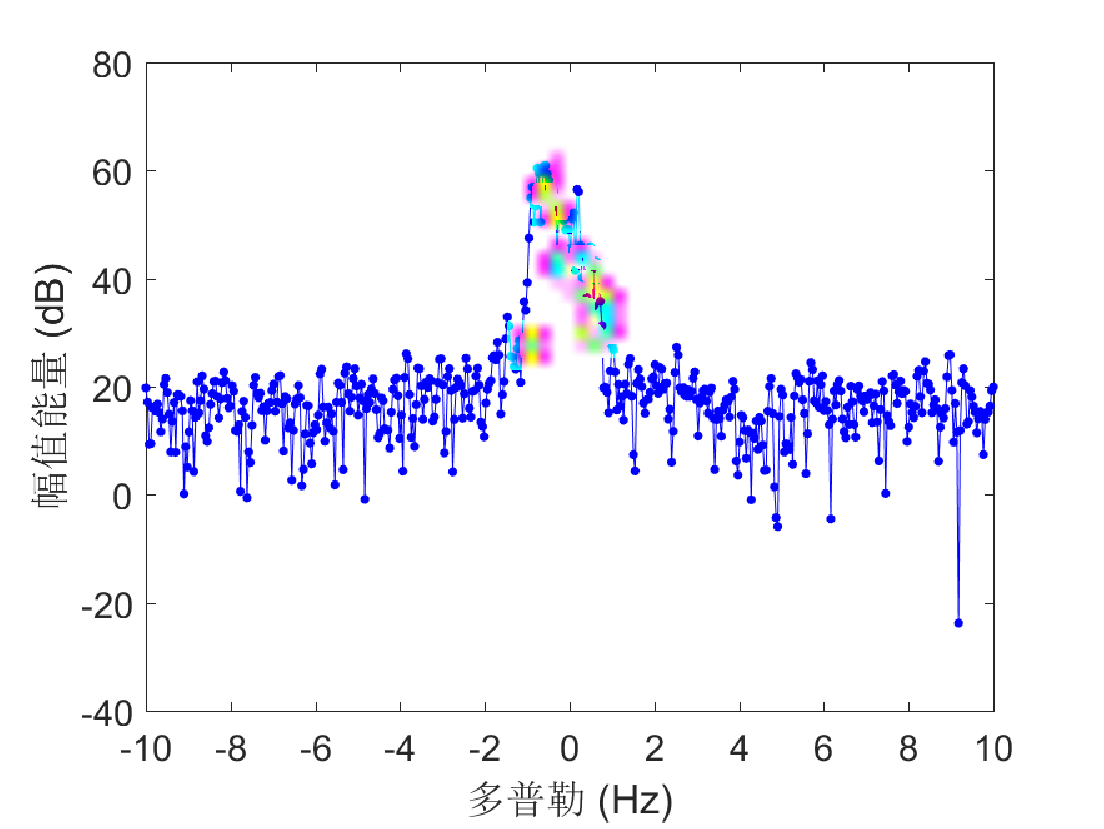
\includegraphics[width=6.67cm]{figures/othr/heatmap}
	\caption{特征重要程度热力图}
	\label{fig:vis}
\end{figure}
% \begin{figure}[H]
% 	\centering
% 	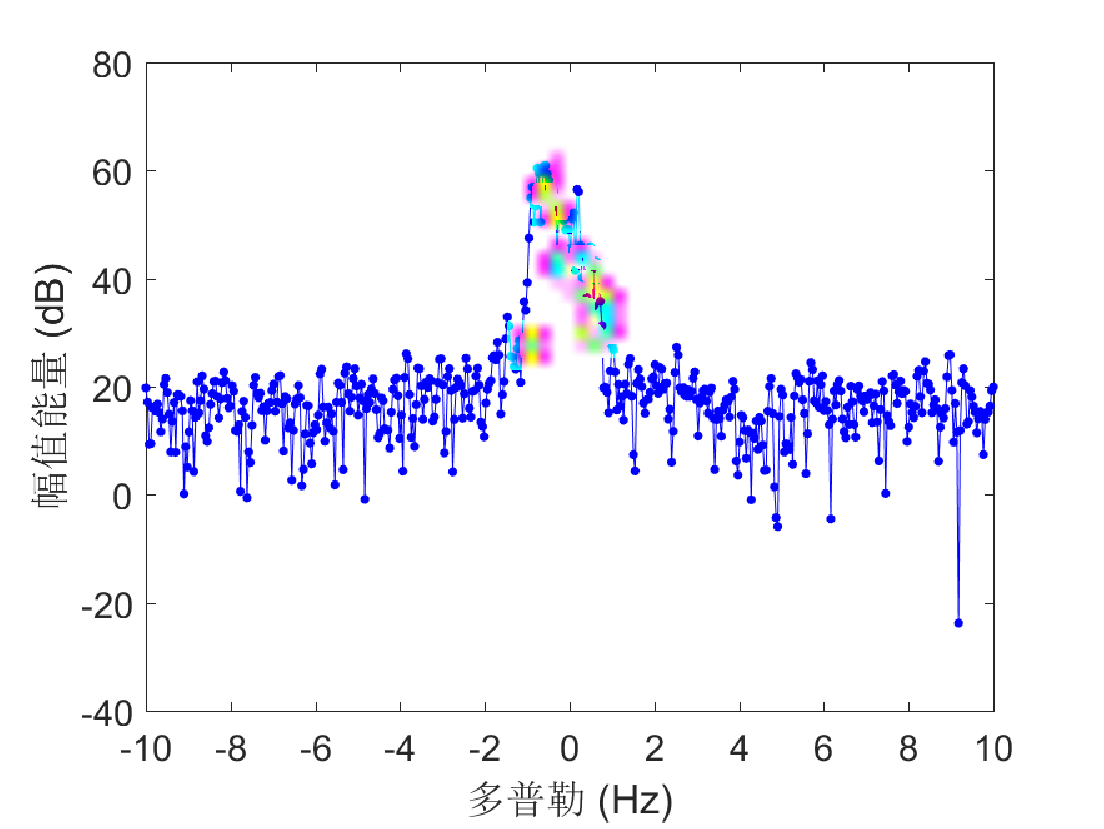
\includegraphics[width=6.67cm]{figures/othr/heatmap.pdf}
% 	\caption{某距离方位单元海杂波频谱数据关注度图。}
% 	\label{fig:visfeature1D}
% \end{figure}

% \textcolor{red}{
% 	识别结果的理论分析
% 	图\ref{fig:visfeature1D}中红色圆圈部分表示主要利用的特征所在多普勒频率,可以很直观地看出,对于图 xxx 这样的海杂波布拉格峰附近频点的数据被关注比较多,另一方面同时兼顾了其余频点的特征,提高了识别准确率。
% }
% 利用我们已经训练好的模型展示对于其最终判断测试结果为正或者为负主要利用的频谱特征点。

\section{小结}
在本章中,我们提出了基于卷积神经网络天波雷达地海杂波识别的新算法。其主要克服了传统的阈值识别方法或支持向量机算法根据经验从频谱数据中提取特征,导致操作复杂度高,分类精度低的缺点。同时,我们将我们的算法与传统算法和支持向量机算法进行了对比,实验结果表明,我们的方法在地海杂波识别问题上更加有效以及抗干扰性能更强,发现利用不同时间的同一区域的频谱数据进行融合可以很大程度上提高分类精度。在更高精度的识别结果的帮助下,我们可以得到更加精确的修正系数,可以为目标定位问题提供非常大的帮助。另一方面,如果我们针对于特定的问题对卷积神经网络的参数进行调整,可以进一步提高我们算法的性能。

% 综上所述,我们这里的创新点有以下两个方面:第一个是我们提出了一种使用深度卷积神经网络方法利用频谱数据进行地海杂波分类的方法,克服了传统算法的挑战;另一方面,我们利用实际数据进行验证


% \subsection{增量学习}
% 随着时间的迁移,天波超视距雷达的观测范围或者是运行参数可能会发生大的变化,使得目前的训练结果无法很好的满足新的需求,于是本文设计了一种基于增量学习的训练方法。对于新的频谱数据集一般会相比于原数据集更小,所以重新训练常常无法取得一个很好的结果,对原始训练结果进行微调是十分必须的。一般来说,DCNN的比较靠前的层所包含的特征更一般化,而更靠后的层会越来越特定于该频谱数据中包含的分类细节。所以一个比较好的方案是保持前面的一些层固定,只微调网络后面的一些层。另一方面,由于原始数据训练出的DCNN的权重是相对较好的,故需要给正在被微调的DCNN权重使用较小的学习率和学习衰减率。
\chapter{基于深度学习的辐射源识别}
% TODO:增加内容与仿真!!!
% 对比利用不同的,添加具体参数的设置。


% 可以考虑进行未经过模糊函数处理和处理之后的对比

% 不同卷积核  学习率  不同卷积核个数
% 层数 节点数等
% 不同训练方法
% 多类别的分类结果图可以参考
% 不同数据的各自的图

\section{引言}
% \textcolor{red}{5923/9500}

辐射源识别算法需要可以准确区分出已知目标和未知目标,同时可以正确的对于已知目标进行分类。我们需要在未收集大量数据的前提下,可以迅速的识别出新的目标。与传统的利用已知类别的样本进行训练测试的机器学习算法不同,辐射源识别的问题是在Open Set的背景下,需要考虑输入未知分类样本的情况。由于复杂电磁环境下辐射源个体识别所面临的识别能力差等问题与挑战,传统辐射源识别方法具有很大的局限性,我们需要寻找一种新的方法解决该问题。

本章综合雷达信号处理、深度学习等多学科理论,详细分析不同辐射源雷达信号的差别,研究不同雷达的信号建模过程以及据此获取雷达信号的基本特征;综合考虑各种脉内细微特征,利用深度卷积神经网络与支持向量机进行结合,以雷达信号的模糊函数切片作为训练样本的特征向量,构建了一个可以对未知分类进行辨识的分类器。最后,利用实际数据进行验证,证明我们的分类器具有很高的准确性。

本章安排如下: 4.2节对辐射源信号进行了分析,并对其进行预处理,求取其模糊函数切片,4.3节构建了本章的Open Set 分类器,详细地阐述了深度卷积神经网络这个主分类器与支持向量机Meta分类器的设计过程,4.4节利用实际数据对于分类器已知分类识别和未知分类辨别的性能进行了验证,4.5节进行本章总结。

% \textcolor{red}{;对雷达有意调制和无意调制这两种脉内调制形式进行建模,综合分析其对应的各种特征(瞬时自相关、相位差分法、模糊函数等建立基于深度学习的分类结构;结合大量数据,对结构进行验证和调整;基于实际数据,对算法的各种特性进行验证。}

\section{辐射源信号分析}
对于辐射源信号的分析处理,本章主要考虑两方面:信号预处理、特征提取优化。
本章所获得的信号为雷达辐射源的I/Q两路数据,这是一种在雷达信号处理领域常见的用来描述信号的方法。其中I表示In-Phase,即同相,Q表示Quadrature,即正交,与I相位之差为90度。
设需要表示的信号的峰值幅度为$A$、相位角为$\phi$,则有:
\begin{equation}
	I = A\cos{\phi}
	\label{equ:i}
\end{equation}
\begin{equation}
	Q = A\sin{\phi}
	\label{equ:q}
\end{equation}
也即,可以利用\equref{equ:signal}表示信号:
\begin{equation}
	Ae^{i\phi}=A(\cos(\phi) + i\sin(\phi))=I+Qi
	\label{equ:signal}
\end{equation}
从而可以根据\equref{equ:i}和\equref{equ:q}利用I、Q数据求取信号的峰值幅度和相位角:
\begin{equation}
	A=\sqrt{I^2+Q^2}
\end{equation}
\begin{equation}
	\phi=tan^{-1}(Q/I)
\end{equation}

在完成信号形式的转换后,我们首先需要对信号进行初步的预处理,剔除无用和错误的数据。

% 从中选取三个类别的I/Q信号图,得到如图 \ref{fig:IQs} 所示,从中可以看出各个信号之间的差距并不明显,因此我们对原始信号进行了优化。

在特征提取优化方面,合理的特征是分类识别的基础。由于存在相同型号的辐射源,利用简单的参数特征无法很好的完成辐射源的个体识别,但是在实际中辐射源自身存在相位噪声以及各类杂散输出,此部分特征可以用来区分出型号、参数均相同的辐射源,因此我们需要选取一种可以提取雷达辐射源这种无意调制产生的信号脉内细微特征的方法。
模糊函数不仅能描述辐射源信号的分辨特性与模糊度,还能描述由雷达辐射源信号所决定的测量精度、杂波抑制特性等,通过模糊函数在时延和频偏这两个维度上的变换,可以多角度的刻画出无意调制对于发射信号的影响,因此我们最终选取了利用雷达模糊函数挖掘辐射源的特征。

\subsection{模糊函数}
对于信号$x(t)$,其瞬时自相关函数为$R_x(t,\tau)=x(t+\tau/2)x^{*}(t-\tau/2)$,其中$\tau$为时延,模糊函数的定义为,
\begin{equation}
A(\tau,\nu) = \int_{-\infty}^{+\infty}R_x(t,\tau)e^{j2\pi\nu t}dt
\label{equ:defineaf}
\end{equation}
即$R_x(t,\tau)$关于时间$t$的傅里叶反变换。

为了方便在数字信号中使用,\equref{equ:defineaf}可以经过变换等价于下面的形式:
\begin{equation}
A(\tau,\nu) = \int_{0}^{\tau}x(t)x^{*}(t+\tau)e^{j2\pi\nu t}dt
\label{equ:afcon}
\end{equation}
对信号均匀采样,即对接收信号和参考信号离散化后,\equref{equ:afcon}可以表示为:
\begin{equation}
A(\tau_l,\nu_m) = A(l, m) = \sum_{n = 0}^{N-1}x(n)x^{*}(n+l)e^{\frac{j2\pi m n}{N}}
\end{equation}
其中,$\tau_l=l/f_s$、$\nu_m=mf_s/N$。

我们此处以一个简单的单载频矩形脉冲信号来展示模糊函数特征提取的作用,图\ref{fig:danpinmaichong}为模糊函数图,可以发现模糊函数存在一定的冗余,其主要变化均处于0时偏和0频偏附近。
为了减小计算量,本章在频偏为0附近取不同时间延迟的切片作为信号特征,即可以有效地提取信号的相位噪声和杂散输出等个体特征,并且此处受噪声的干扰较小,更加稳定,图 \ref{fig:qiepian}即为在频偏为0处的单载频矩形脉冲信号模糊函数切片。

\begin{figure}[hbt]
	\centering
	\begin{minipage}[b][][b]{7cm}
		\centering
		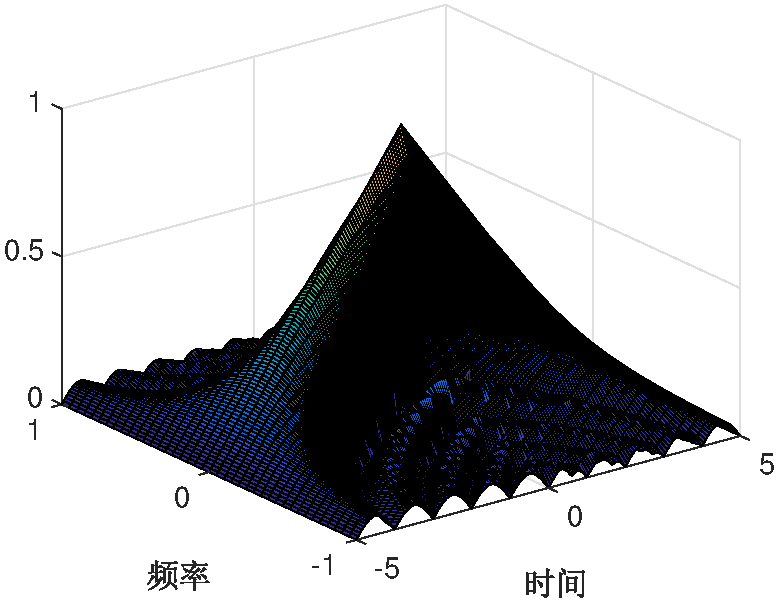
\includegraphics[width=6.67cm]{figures/emitter/danpinmaichong}
		\caption{单载频矩形脉冲信号模糊函数图}
		\label{fig:danpinmaichong}
	\end{minipage}
	\hspace{10pt}
	\begin{minipage}[b][][b]{7cm}
		\centering
		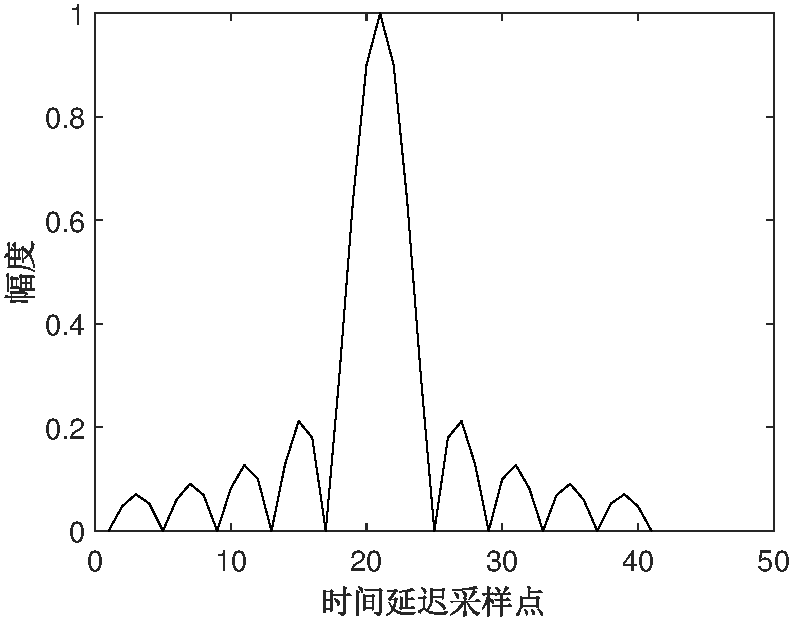
\includegraphics[width=6.67cm]{figures/emitter/qiepian}
		\caption{单载频矩形脉冲信号模糊函数切片}
		\label{fig:qiepian}
	\end{minipage}

\end{figure}


\section{Open Set 分类器设计}
通常的识别或者分类系统仅考虑的是一个闭集分类系统,然而在现实世界中,这种分类系统会遇到很大的问题。由于其最基本的假设是所有的类别均为先验已知,那么就会出现问题,例如在训练样本中不存在类别的样本就会被错误的分到某个类别中去。这种在训练的时候提供不完整的信息,而在测试的时候会添加未知分类的问题,称作Open Set 识别\ucite{scheirer2013toward, jain2014multi}。这个问题还可以描述为需要在测试的时候拒绝未知样本。Open Set目标识别系统必须可以准确的处理下面三种类型的数据类:
\begin{itemize}
	\item 已知的(目标)类,被标记为正训练样本的数据。
	\item 已知的未知(非目标)类,被标记为负训练样本的数据。
	\item 未知的未知(非目标)类,在训练样本中不存在的类别的数据。
\end{itemize}
传统的机器学习算法均为针对于闭集数据设计的,随着识别算法应用场景的增多和对精度要求的提高,许多学者开始了对Open Set识别的研究。Simonson\ucite{simonson1998probabilistic}提出了一种称作概率融合(probabilistic fusion, PF)的利用统计的方法来进行Open Set识别,其主要通过合并来自不同数据源的证据得到一个统计测试模型,根据此模型的分布来对于类别进行判断。Scheirer等人\ucite{scheirer2011meta}提出了一种通过分析后验数据得分来进行类型判断的方法。

此部分主要解决的问题是当得到一个新的测试样本,如果该样本不属于已经经过训练的分类,那么传统的神经网络模型会将该样本指派给与其最相似的一个类别,此种情况对于一个Open Set识别系统,也即类似于辐射源识别系统这种具有较多尚未经过训练的样本的一个数据集,首先这会导致其识别率下降,另一方面是由于对于未知的辐射源无法很好的确定,无法很好的完成预警等任务。目前,学者对于该问题的研究主要分为下面两个思路:
\begin{itemize}
	\item 在训练集中添加一个“未知”类别,利用不同的来自非已知类别的数据作为训练样本对该类别进行训练,然后对于所有的输入数据进行类别的识别,对于识别结果为该类别的数据作为未知分类。
	\item 针对于多分类使用的softmax函数,可以设立阈值或者对于该识别结果进行一个评价(例如与已知类别数据的一个“距离”),通过这种方式分辨出未知分类。
\end{itemize}
第一个思路最大的问题是我们无法得到所有可能的未知类别的样本来进行训练,具有一定的局限性,不适用于我们这个具有大量来自未知分类数据的问题。针对于该问题,我们基于后一个思路设计了一个基于Meta-Recognition的可以识别未知辐射源的深度神经网络。首先是创建一个深度卷积神经网络分类器,该分类器的输出为该训练样本属于各个类别的概率,我们然后将此类别作为一个输入,输入到我们的Meta-Recognition中,这里我们设计一个支持向量机分类器作为Meta-Recognition,然后从该Meta-Recognition会进行判断该输入是否为一个未知分类。
\begin{figure}[hbt]
	\centering
	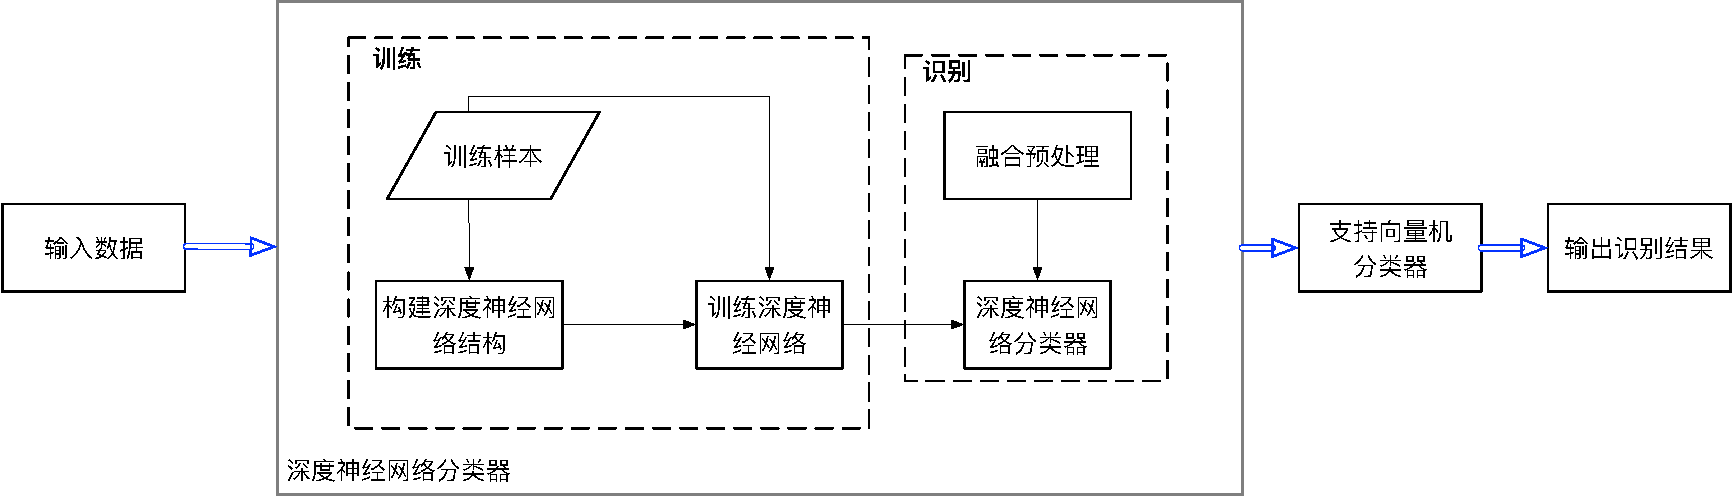
\includegraphics[width=13.5cm]{figures/emitter/frame_emitter}
	\caption{分类器设计结构图}
\end{figure}

\subsection{深度卷积神经网络分类器设计}
本章根据辐射源信号的实际数据以及其反映出来的特性,设计构建了一个具有10层的一维卷积神经网络。

该分类器作为主要分类器,且Meta-Recognition是以该分类器的输出作为输入,所以该分类器性能的好坏会直接影响到对已知类别的分类和对未知类别的判断。

第一层是输入层,由于模糊函数切片为一个$1 \times 1000$的向量,因此输入层大小是$1 \times 1000$。

第二层是卷积层$C1$,$C1$对输入向量进行一维卷积运算提取特征,卷积运算可以最
大程度的提取原始信号的特征。此处利用了256个大小为$1\times 3$的卷积滤波器,其窗口移动步长为1。

第三层是一个池化层$S2$,$S2$层对上一层$C1$做池化处理,池化的目
的是在保留数据有用信息的同时,尽可能减少数据量。此处采用的是$1\times 2$的最大池化操作。

第四层是一个卷积层 $C3$,$C3$对$S2$的特征进行卷积操作,此处利用了128个大小为$1\times 3$的卷积滤波器。

第五层是一个卷积层 $C4$,其结构与$C3$相同,128个大小为$1\times 3$的卷积滤波器。

第六层是一个池化层 $S5$,其结构与$S2$相同,$1\times 2$的最大池化操作。

第七层是一个卷积层 $C6$,其结构与$C3$相同,128个大小为$1\times 3$的卷积滤波器。

第八层是一个卷积层 $C7$,其结构与$C3$相同,128个大小为$1\times 3$的卷积滤波器。

第九层是一个池化层 $S8$,其结构与$S2$相同,$1\times 2$的最大池化操作。

第十层是输出层,根据不同的类别个数选取相应的输出节点个数,首先将$S8$的特征拉成一个一维向量,然后通过全连接网络与输出层进行连接,通过Softmax激活函数输出最终的结果。


% 第五层是一个下采样层 S 4,S  4和 S 2是一样的,也是采用2  2邻域,那么 S4
% 层 12 个特征图,每一个特征图大小是4  4。
% 第六层是输出层,由于样本标签一共有 10 个,那么输出层是 10 个节点,
% 算法将 S 4层的所有特征图拉成一个一维向量,然后与输出层直接相连,这里的
% 相连是全连接。

% \textcolor{red}{这部分缺少详细描述,但是如何和上一个问题区分开来是一个问题}

\begin{figure}[hbt]
	\centering
	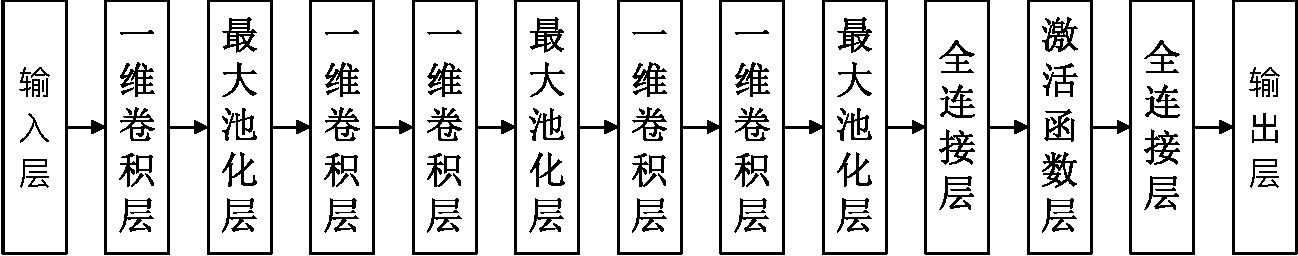
\includegraphics[width=13.5cm]{figures/emitter/struct_emitter}
	\caption{深度卷积神经网络框架图}
\end{figure}

\subsection{支持向量机 Meta-Recognition 设计}

\subsubsection{支持向量机原理}
支持向量机是一种流行的分类方法,它可以在不需要大量数据的情况下产生良好的结果。对于一个二分类问题,设$((x_1,y_1),\dots,(x_n,y_n))$为训练数据集,其中$x_i$为某样本的特征向量,$y_i\in\{-1,+1\}$为该样本的标签。支持向量机的思想为找到一个超平面将这些样本划分为正类(标签为$+1$)和负类(标签为$-1$),并且使得正类和负类之间的距离最大。这个超平面的间隔被定义为正类与负类之间的最近距离。

对于一个线性分类问题,假设所有的数据满足下面的约束:
\begin{equation}
	w\cdot x_i +b \geq + 1 \quad y_i = +1
	\label{equ:constraint1}
\end{equation}
\begin{equation}
	w\cdot x_i +b \leq + 1 \quad y_i = -1
	\label{equ:constraint2}
\end{equation}
其中$w$为超平面的法向量,$\frac{|b|}{||w||}$是从超平面到原点的垂直距离,$||w||$是向量$w$的欧拉范数。将上述两个式子合并得到:
\begin{equation}
	y_i(w\cdot x_i+b)\geq 1 \forall i
	\label{equ:svm}
\end{equation}
\equref{equ:svm} 中的训练样本构成了这个分类平面(图 \ref{fig:hyperplanes} 中的$H_1$与$H_2$)。间隔 $\rho$ 可以通过计算$H_1$与$H_2$的距离得到:
\begin{equation}
	\rho=\frac{|1-b|}{||w||}-\frac{|-1-b|}{||w||}=\frac{2}{||w||}
\end{equation}
\begin{figure}[hbt]
	\centering
	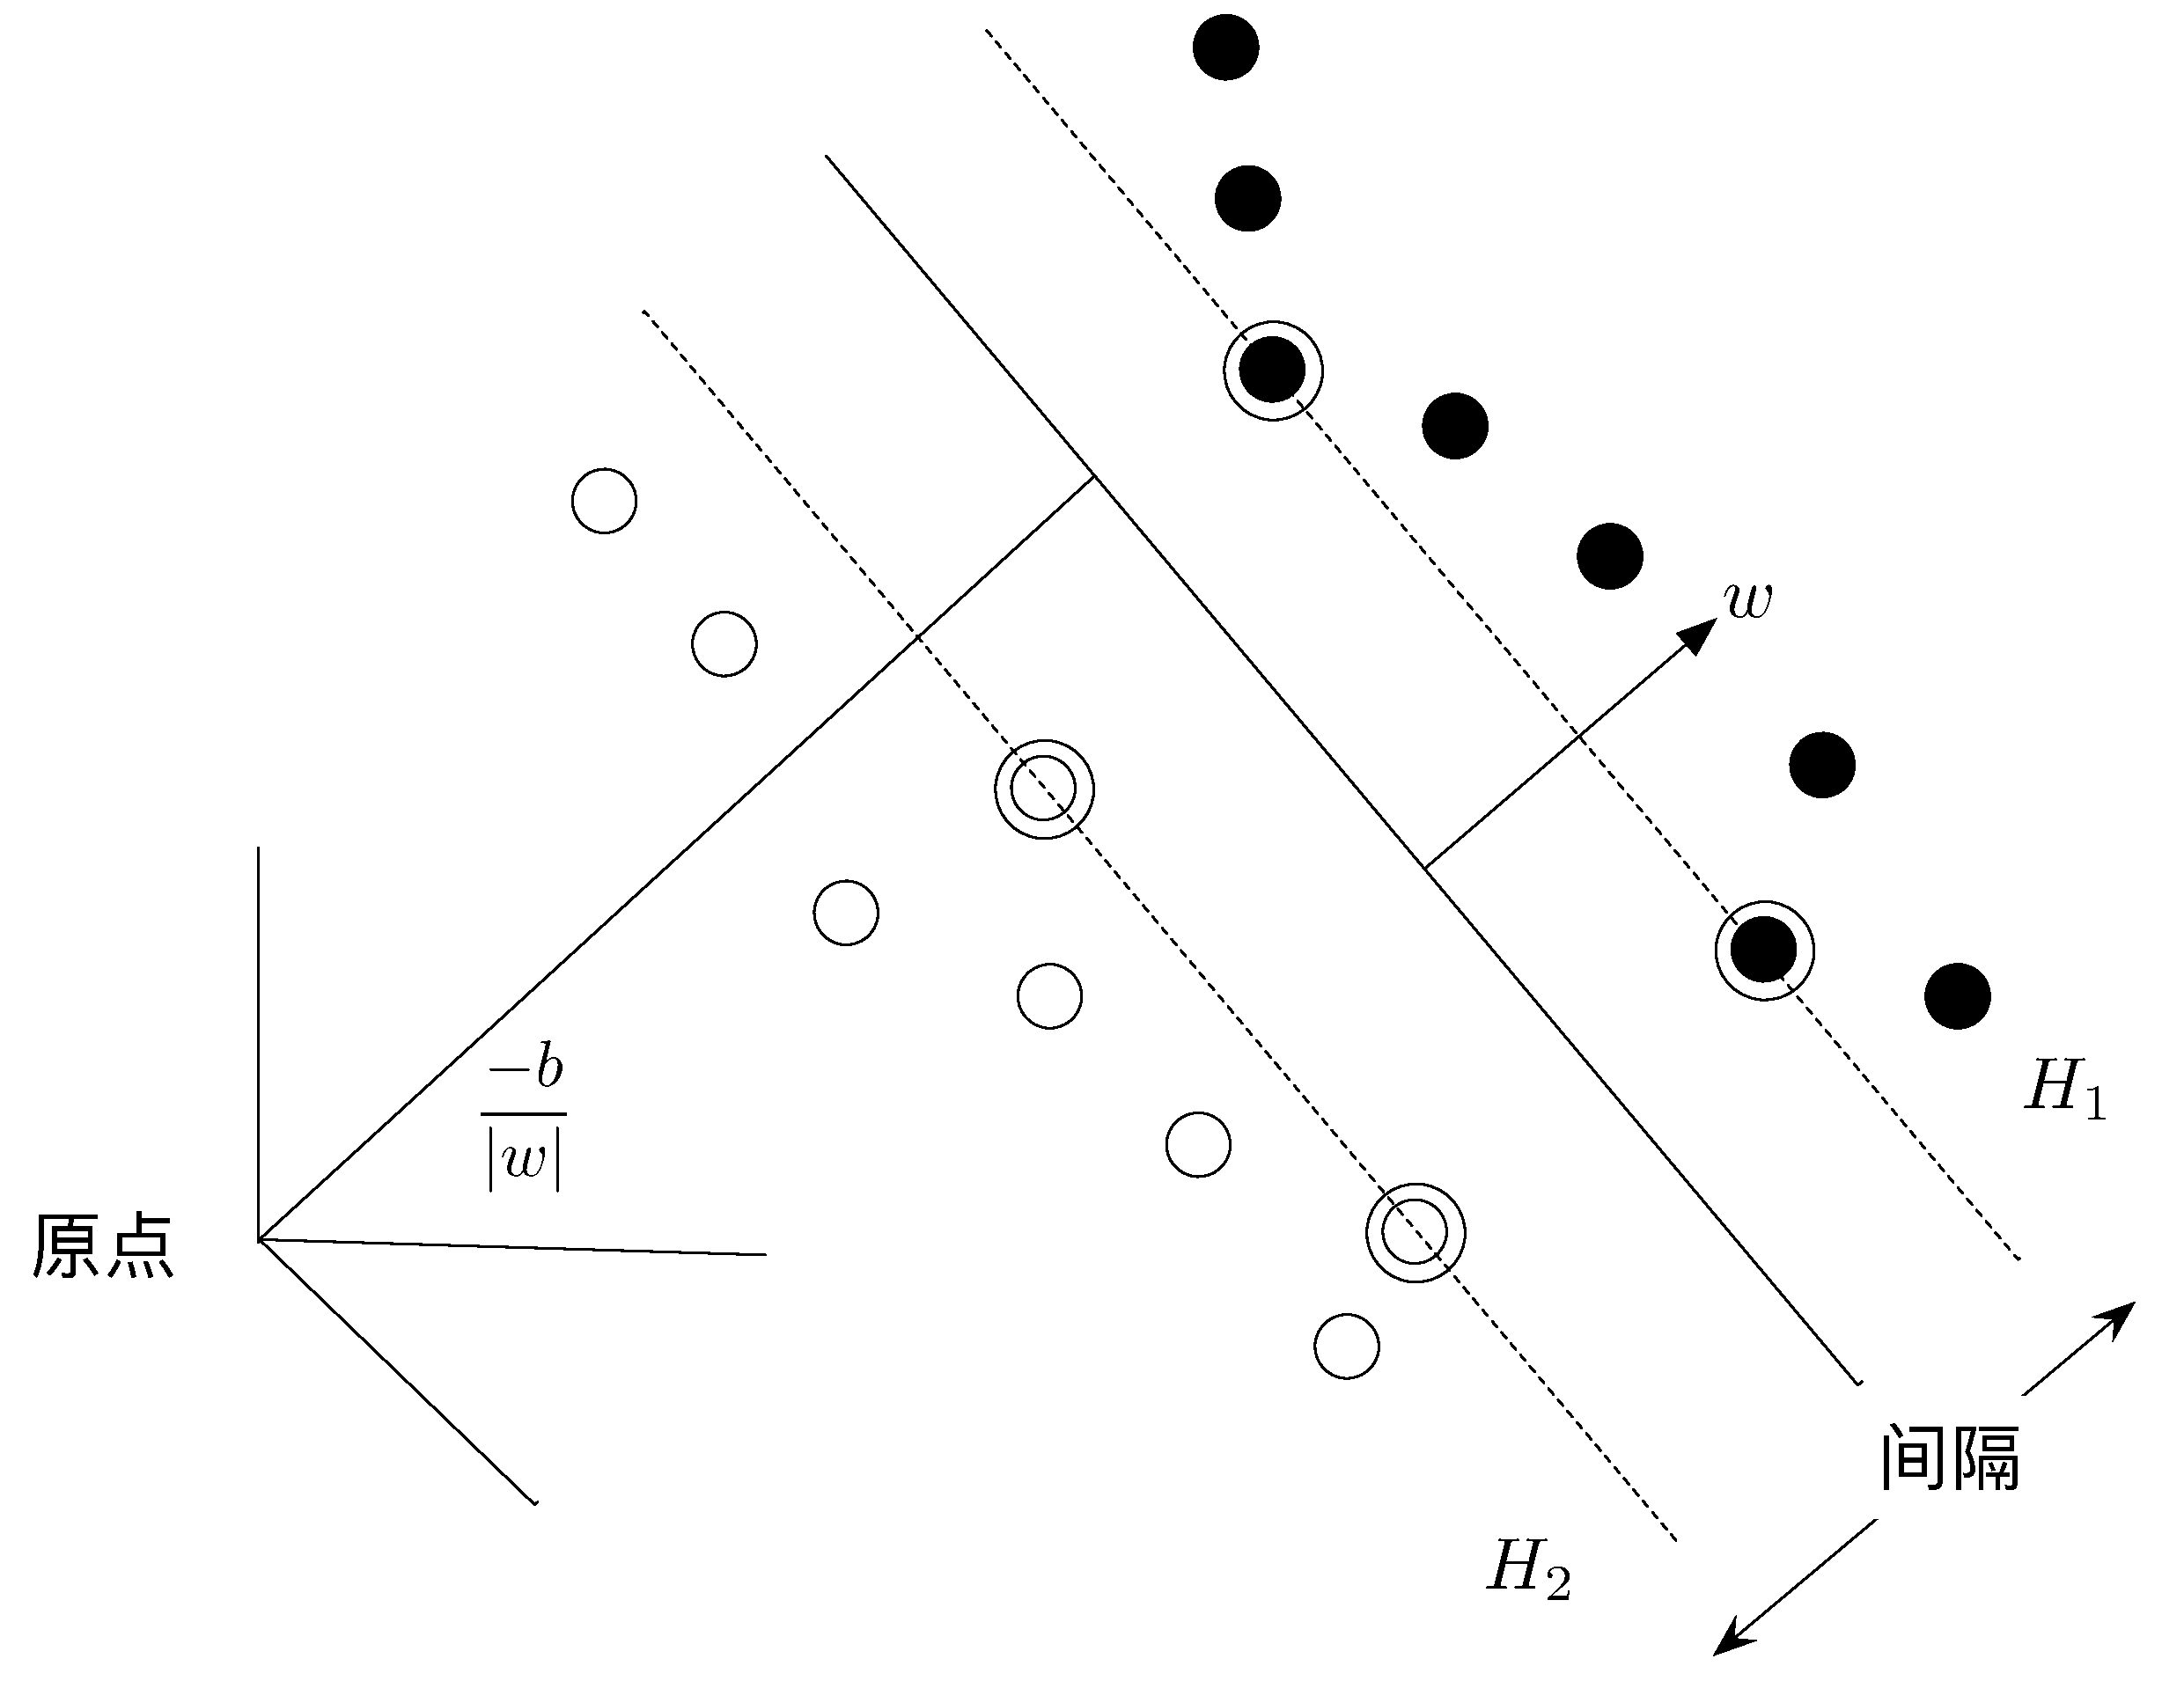
\includegraphics[width=6.67cm]{figures/emitter/svm_hard}
	\caption{标准分类平面,即具有最大间隔的超平面。被圈起来的样本组成了这个超平面,其被称作支持向量。}
	\label{fig:hyperplanes}
\end{figure}
因此求解标准分类超平面的最大间隔的问题,就转变为下面的优化问题。
\begin{equation}
	\min \limits_{w\in \mathcal{H}} \tau(w)=\frac{1}{2}||w||^2\quad s.t. \quad y_i(w\cdot x_i +b) \geq 1 \quad \forall i
	\label{equ:optimization}
\end{equation}

为了使得约束更好表示,我们用拉格朗日优化算法对上式重新描述,
\begin{equation}
	\min \limits_{w,b} L(w,b,\alpha)=\frac{1}{2}||w||^2-\sum_{i=1}^l\alpha_i y_i (x_i w + b) + \sum_{i=1}^l{\alpha_i}
	\label{equ:lagrange}
\end{equation}
其中$\alpha_i \geq 0$为约束条件。

在实际计算过程中,我们通过对偶定义求解优化方程\equref{equ:lagrange},通过最大化方程\equref{equ:lagrange}相对于$\alpha$来求取其相对于$w$和$b$的最小值。利用 Karush-Kuhn-Tucker 条件,则\equref{equ:lagrange}变为下面对偶形式:
\begin{equation}
	\max \limits_{\alpha} L_D=\sum_i{\alpha_i}-\frac{1}{2}\sum_{i,j}\alpha_i\alpha_jy_iy_jx_i\cdot x_j \quad s.t. \quad \forall i
	\left\{
		\begin{aligned}
	   &\sum_i{\alpha_iy_i}=0  \\
	   &\alpha_i \geq 0
	   \end{aligned}
		\right.
\end{equation}
因此,通过求解这个对偶优化问题,可以得到系数$\alpha_i$。其中满足$\alpha_i>0$的解称作支持向量,他们位于标准分类平面$H_1$或者$H_2$上。注意到,仅有$\alpha_i>0$的解影响最终的支持向量的选择。
因此,可以得到决策函数:
\begin{equation}
	f(x)=w^Tx_i+b=\sum_{i=1}^My_i\alpha_i(x_i^Tx)+b
\end{equation}
决策函数的符号取决于预测样本$x$。

此处我们讨论的情形的一个假设是,我们可以把所有的样本完全分为不同的类别。但是显然在大多数情况下,这种假设是不成立的。另外,这种假设也会导致过拟合现象的出现。因此,文献 \cite{cortes1995support} 提出了软间隔的支持向量机。
其基本思想是,通过引入正的松弛变量$\xi_i$来放宽\equref{equ:constraint1}和\equref{equ:constraint2}的约束。基于此,得到\equref{equ:constraint_soft}

\begin{equation}
	\forall i \quad
	\left\{
	 \begin{aligned}
	&w\cdot x_i + b \geq +1-\xi_i \quad y_i=+1  \\
	&w\cdot x_i + b \leq -1-\xi_i \quad y_i=+1  \\
	&\xi_i \geq 0
	\end{aligned}
	 \right.
	\label{equ:constraint_soft}
\end{equation}
这允许一些样本在边缘内部,甚至在相反类别的情况下进一步交叉(见图\ref{fig:softmargin})。 虽然这种松弛使得支持向量机能够灵活地降低异常值的影响,但是从优化问题求解的角度来看,我们不希望有任意大的松弛变量$\xi_i$,因为这会导致SVM获得平凡和次优的解。 因此,我们通过使松弛变量成为\equref{equ:optimization}的一部分,来限制松弛度:
\begin{equation}
	\min \limits_{w\in \mathcal{H},\xi\in \mathbb{R}^m} \tau(w,\xi)=\frac{1}{2}||w||^2+C\sum_{i=1}^m {\xi_i}
\end{equation}
\begin{figure}[hbt]
	\centering
	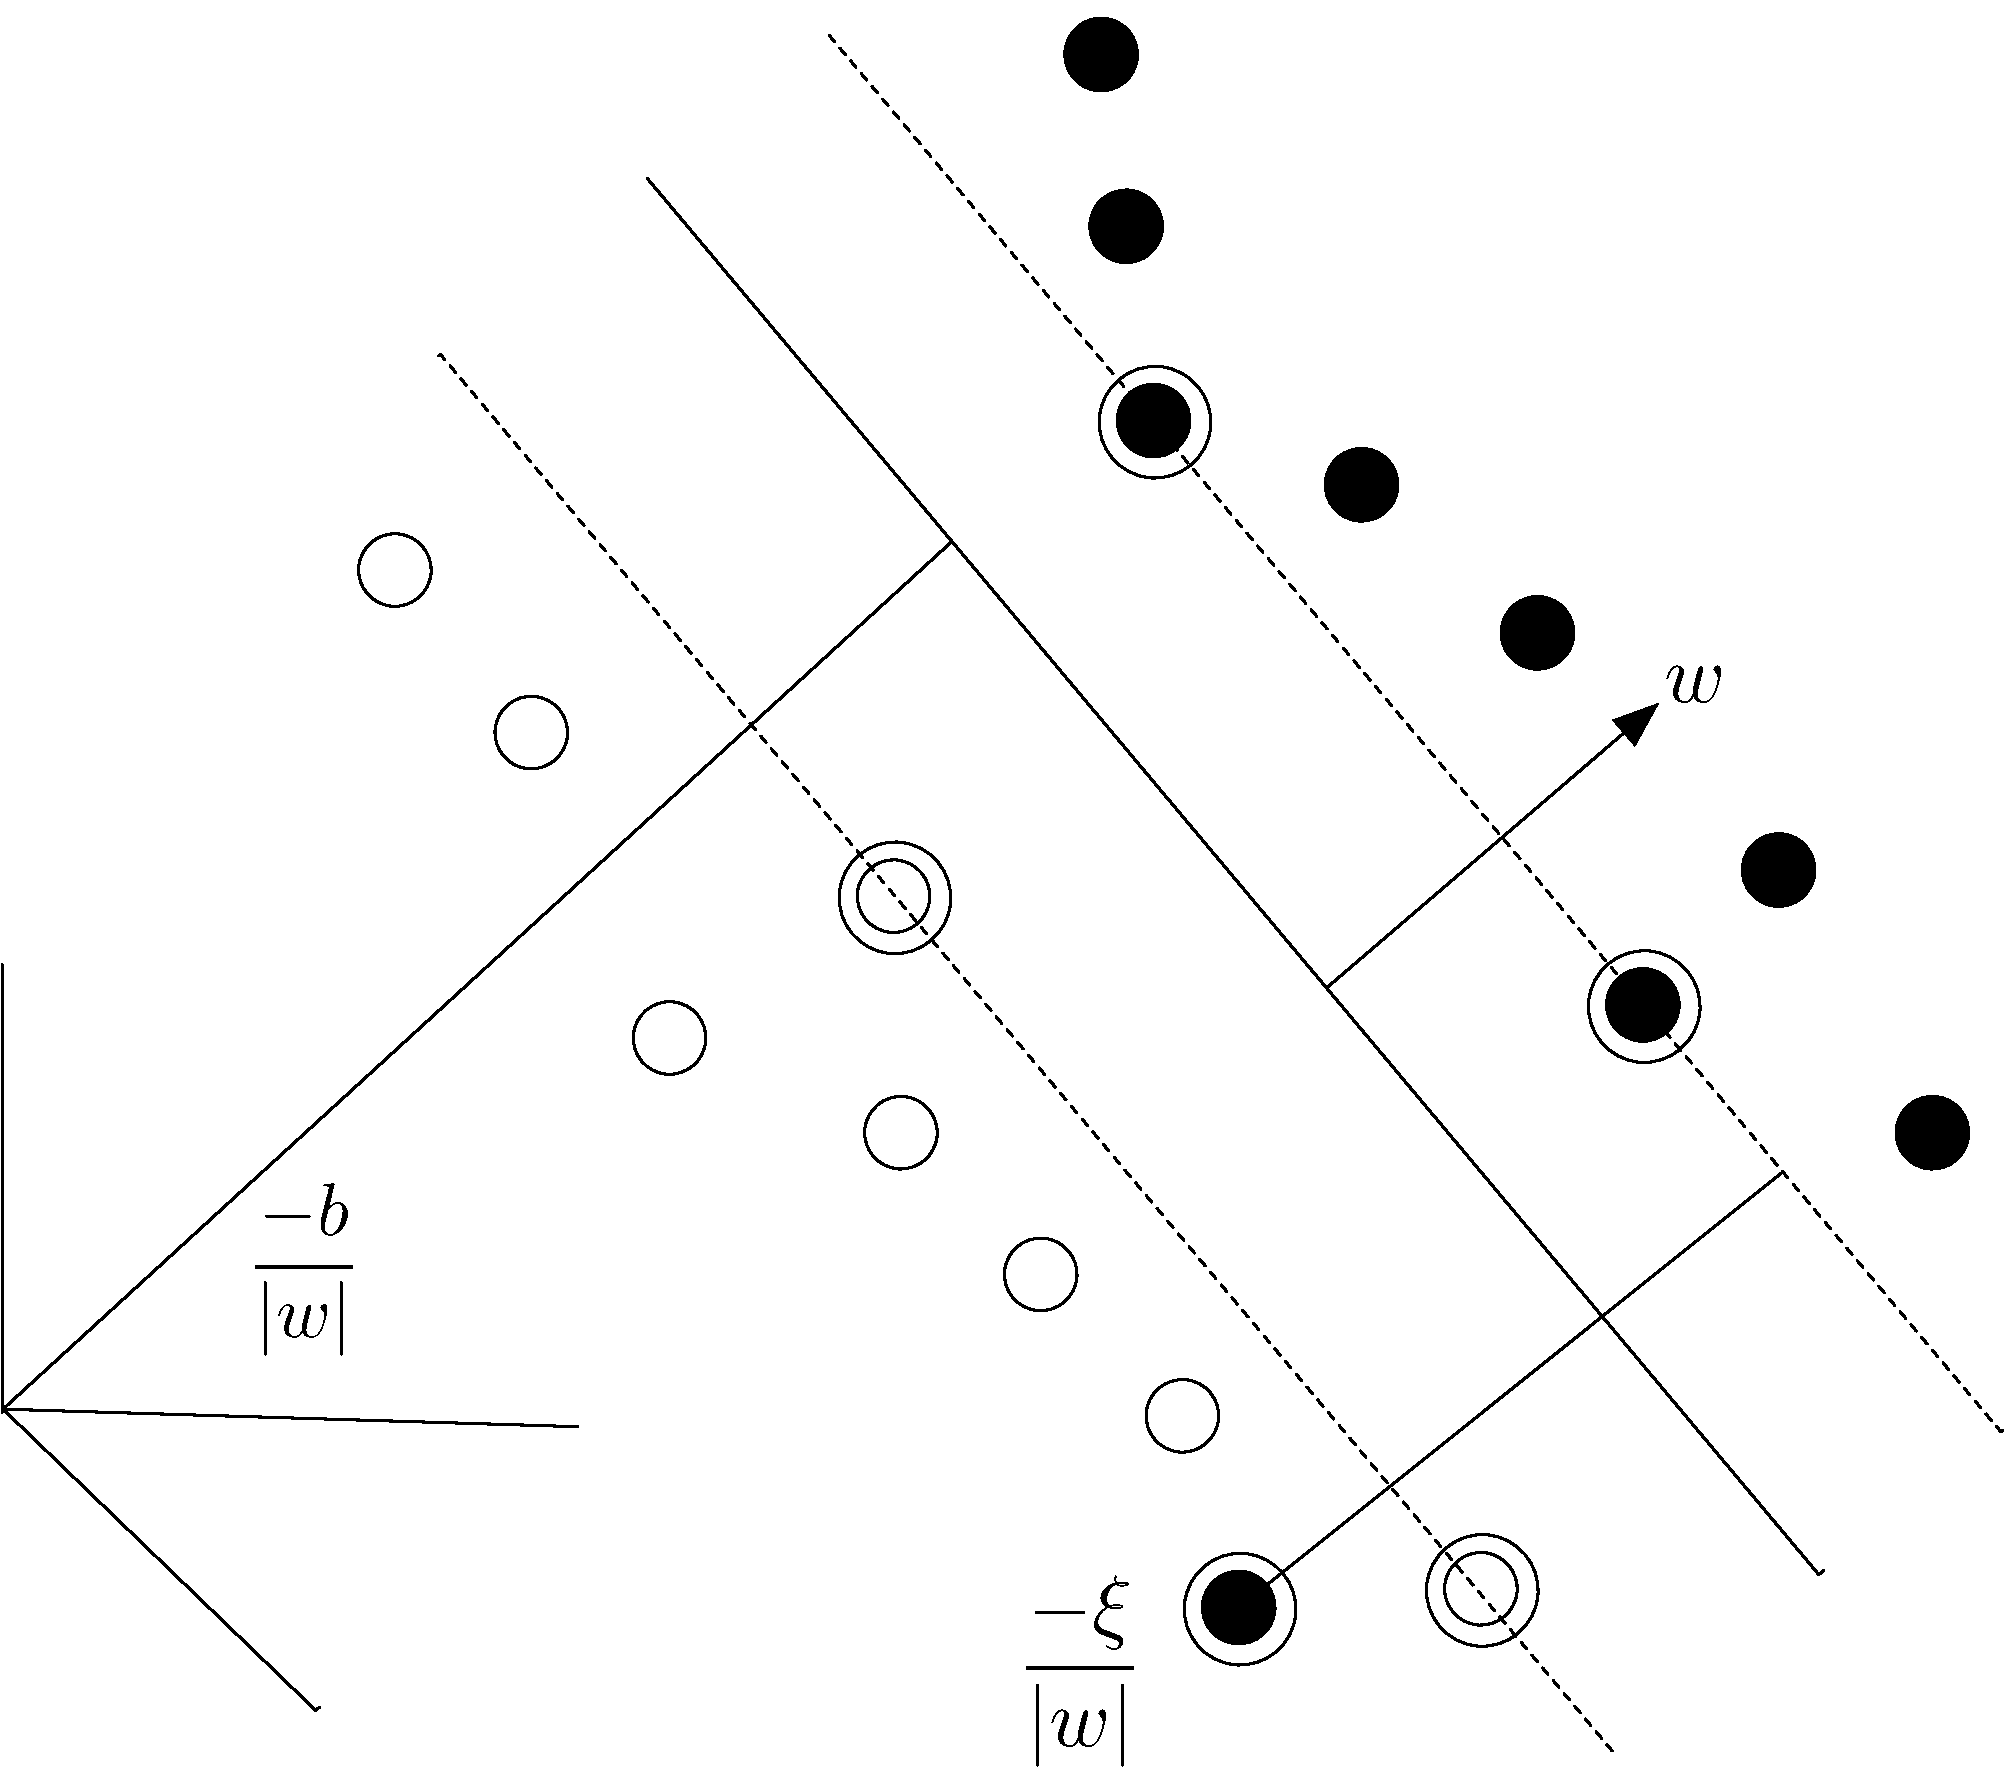
\includegraphics[width=6.67cm]{figures/emitter/svm_soft}
	\caption{软间隔支持向量机}
	\label{fig:softmargin}
\end{figure}
其约束条件为\equref{equ:constraint_soft}。超参数$C>0$是针对于误分类的惩罚系数,该系数需要根据不同的分类任务和数据集进行调整。
将其变为的对偶形式,则有
\begin{equation}
	\max \limits_{\alpha} L_D=\sum_i{\alpha_i}-\frac{1}{2}\sum_{i,j}\alpha_i\alpha_jy_iy_jx_i\cdot x_j \quad s.t. \quad \forall i
	\left\{
		\begin{aligned}
	   &\sum_i{\alpha_iy_i}=0  \\
	   &C \leq \alpha_i \geq 0
	   \end{aligned}
		\right.
	\label{equ:cdotdual}
\end{equation}

目前只是分析了线性支持向量机的问题,为了应对非线性分类问题,我们引入了核函数的概念。将训练数据通过某函数$\Phi:\mathbb{R}^d\mapsto\mathcal{H}$。经过该变换后,我们只需要将原来计算$\mathbb{R}^d$的$x_i\cdot x_j$变换为计算在$\mathcal{H}$域的向量积$\Phi(x_i)\cdot\Phi(x_j)$。为了降低计算量,可以引入核函数$K$来避免数据$x_i$和$x_j$从$\mathbb{R}^d$映射到$\mathcal{H}$。
\begin{equation}
	K(x_i,x_j)=\Phi(x_i)\cdot\Phi(x_j)
\end{equation}
因此,可以将\equref{equ:cdotdual}变为:
\begin{equation}
	\max \limits_{\alpha} L_D=\sum_i{\alpha_i}-\frac{1}{2}\sum_{i,j}\alpha_i\alpha_jy_iy_j K(x_i,x_j)\quad s.t. \quad \forall i
	\left\{
		\begin{aligned}
	   &\sum_i{\alpha_iy_i}=0  \\
	   &C \leq \alpha_i \geq 0
	   \end{aligned}
		\right.
\end{equation}
常用的核函数有下面几种:
\begin{itemize}
	\item 线性核函数:$K(x,y)=x^Ty+C$
	\item 多项式核函数:$K(x,y)=(x^Ty+C)^d$
	\item RBF 核函数:$K(x,y)=e^{\frac{-||x-y||^2}{2\sigma^2}}$
	\item Sigmoid 核函数:$K(x,y)=\tanh(\alpha x^Ty+C)$
\end{itemize}
\subsubsection{支持向量机设计}
我们可以利用所有的目标数据和未知目标的数据来作为训练样本对该SVM分类器进行训练,本部分我们以深度卷积神经网络的输出作为该分类器的输入,利用各类别的概率作为其特征进行训练识别。由于在类别的识别过程中,存在一定的波动性,这个会影响对于是否属于未知类别的分类判断,我们这里选取对于来自同一个辐射源的连续10拍的识别结果进行一个平均作为最终的输入。

下面是对于SVM分类器的设计,首先是核函数的选择。核函数将输入空间映射到高维特征空间,最终在高维特征空间中构造出最优分类超平面,从而把平面上本身不好分的非线性数据分开。常用的核函数为线性核函数和径向基核函数( Radial Basis Function, RBF)。对于核函数的选择,一般分为三种情况:
\begin{itemize}
	\item  特征的数量很大,跟样本数量差不多,这时候选用逻辑回归算法或者是线性核的SVM
	\item  特征的数量比较小,样本数量一般,不算大也不算小,选用径向基核函数
	\item  特征的数量比较小,而样本数量很多,需要手工添加一些特征变成第一种情况
\end{itemize}
由于我们的问题符合第二种情况,故选择径向基核函数。

具有径向基核的支持向量机具有两个关键参数,惩罚参数$C$的和核参数$\sigma$,这两个参数的取值在很大程度上决定了SVM的性能的优劣。核函数的参数主要影响样本数据在高维特征空间中分布的复杂程度,即维数。特征子空间的维数越高,那么得到的最优分类超平面就会越复杂。反之亦然。因此只有选择合适的核参数得到合适的特征子空间,才能得到推广能力良好的SVM分类器。大量的实验数据表明,如果与样本点之间的距离很小,$\sigma \rightarrow 0$;如果与样本点之间的距离很大时,$\sigma \rightarrow \infty$;当$\sigma$很小,径向基核函数支持向量机得到的判别函数差不多是一个常数,出现过拟合现象。当$\sigma$很大时,样本的正确分类率也会比较低。

惩罚参数是影响SVM算法性能的另一个重要因素。它的作用主要是调节特征子空间中SVM模型的置信范围与经验风险的比例,使支持向量机的泛化能力达到最好。特征子空间不同时,最优参数值取值也会不同。惩罚参数与经验误差的惩罚和SVM的复杂度成正比,与经验风险值成反比。因此,选择合适的惩罚参数也是非常重要的。

% \textcolor{red}{
% 从上面的分析可以看出,核参数影响着映射函数、进而影响样本子空间的复杂度。最后会影响分类器性能的好坏。惩罚参数作用是在数据子空间中调节支持向量机置信区间的范围。这些都说明了惩罚参数和核参数的选择非常重要。
% }
\section{仿真实验与分析}
\subsection{实验环境}
% \textcolor{red}{关于IQ两路数据的一个叙述}

本章利用了来自13架民航飞机的气象雷达辐射源的数据,飞机信息参见表\ref{tab:flight}
\begin{table}[hbt]
	\renewcommand{\arraystretch}{1.3}
	\caption{辐射源信号数据}
	\label{tab:flight}
	\centering\sWuhao
	\begin{tabularx}{\textwidth}{>{\centering\arraybackslash}X>{\centering\arraybackslash}X>{\centering\arraybackslash}X}
		\toprule
		 飞机地址码 & 飞机航班号 & 飞机型号  \\
		 \midrule
		 7BF014 & CCA1416 & Airbus A330 (twin-jet)\\
		 780DB3 & TBA9881 & Airbus A330 (twin-jet) \\
		 780E06 & CSN3438 & Airbus A330 (twin-jet\\
		 780EBB & CES293 & 	Airbus A321 (twin-jet)\\
		 780EBF & CES2342 & Airbus A320 (twin-jet)\\
		 7804F2 & ZH9164 & Airbus A320 (twin-jet)\\
		 7804F4 & CES5856 & Boeing 737\\
		 7806FC & CSN6402 & Airbus A320 (twin-jet)\\
		 7808F0 & CES5373 & Airbus A319 (twin-jet)\\
		 78057F & CCA4103 & Airbus A321 (twin-jet\\
		 780063 & CCA4377 & Airbus A319 (twin-jet)\\
		 780375 & CSC8253 & Airbus A319 (twin-jet)	\\
		 781022 & EU2731 & Airbus A319 (twin-jet)\\
		 \bottomrule
	\end{tabularx}
\end{table}
对于我们的气象雷达辐射源信号,原始的I/Q数据的示意图如图 \ref{fig:IQ} 所示
\begin{figure}[hbt]
	\centering
	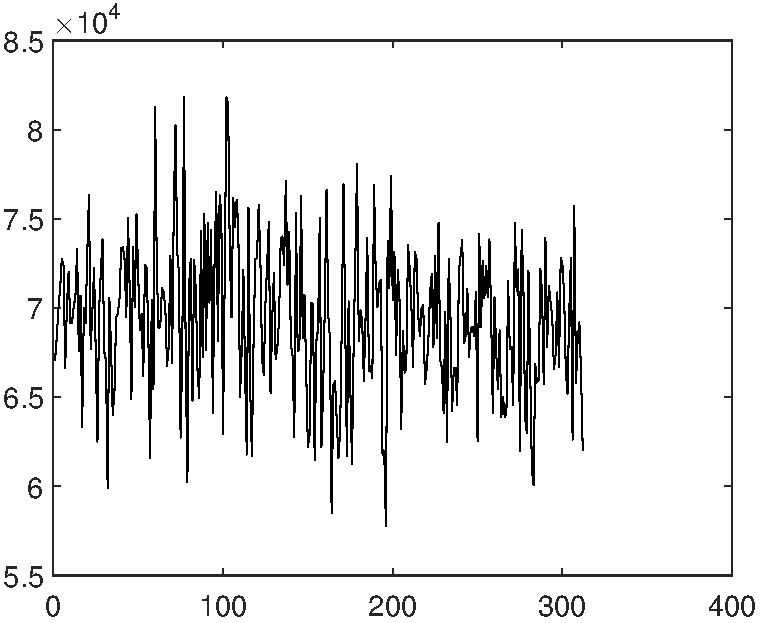
\includegraphics[width=6.67cm]{figures/emitter/IQA}
	\caption{原始I/Q信号}
	\label{fig:IQ}
\end{figure}

原始的雷达信号为I/Q信号,我们将他们利用快速傅里叶变换求取其模糊函数切片作为输入的特征向量。每架飞机原始信号为100次雷达扫描周期的信号,为了增加数据样本数目,我们对原始信号添加噪声生成了新的信号,最终每架飞机均有10000组信号。对于这些信号,我们选择其中的$70\%$作为训练样本,$20\%$用于交叉验证,$10\%$作为测试,同时在测试样本中添加与其等量的来自未训练类别也即未知类别的样本共同作为测试样本用来衡量其未知分类的识别率。

由于我们原始获得的数据为I/Q两路数据,为了更好的捕捉到回波的特征信息,我们对数据进行了一个变换,求取其模糊函数,并做偏移为0附近的一个切片。由于深度学习需要大量的数据进行训练学习,而本身数据量偏少,故我们在已有数据的基础上在一定信噪比的前提下,生成部分仿真数据。

对于数据的选择方面,我们从数据中选择出2至8个类别分别进行实验,对于每一个类别,我们均选择大约10000组数据,其中$70\%$作为训练样本,$20\%$作为交叉验证样本,$10\%$作为测试样本,同时在测试样本中又添加了与已知分类等数量的未知分类的数据进行测试。
\begin{figure}[hbt]
	\centering
	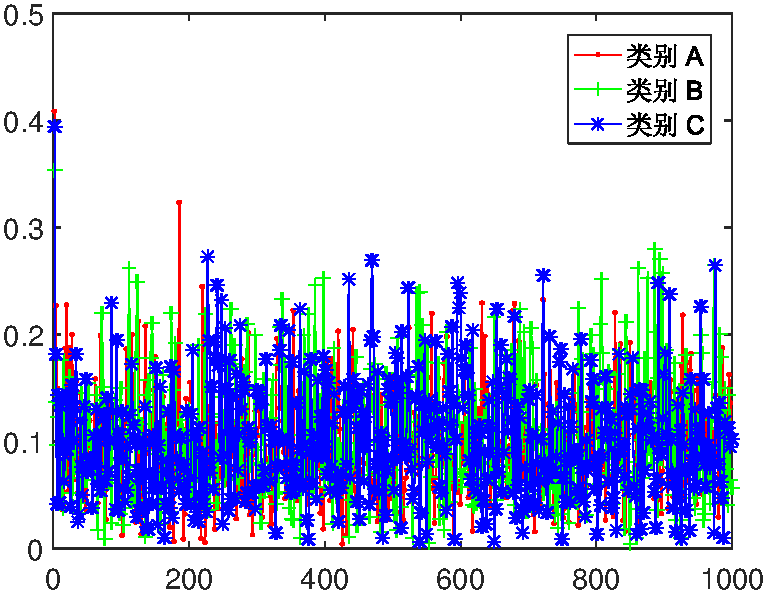
\includegraphics[width=6.67cm]{figures/emitter/diff_data}
	\caption{不同类别样本特征图}
\end{figure}
由于该变换后,数据之间的差距比较大,我们对数据进行了归一化。我们采用的归一化方法为min-max标准化(Min-Max Normalization),也称为离差标准化,是对原始数据的线性变换,使结果值映射到$[0 , 1]$之间。转换函数如下:
\begin{equation}
x^{*}=\frac{x-x_{min}}{x_{max}-x_{min}}
\end{equation}
其中$x_{max}$为样本数据的最大值,$x_{min}$为样本数据的最小值。

我们采用网格搜索法
% \textcolor{red}{网格搜索法}
对SVM参数进行调优,最终选择参数惩罚参数为32,核参数$\sigma$为0.0312。

\subsection{实验结果分析}

\subsubsection{深度卷积神经网络识别结果}

% \textcolor{red}{该部分是否修改为表格,然后注意描述的时候准确表达所运用的数据,该部分主要利用某一个多类别的进行研究。}

首先验证深度卷积算法的识别正确率,利用8个类别的数据进行训练和测试,迭代次数为100次。

\begin{figure}[hbt]
	\centering
	\begin{minipage}{7cm}
		\centering
		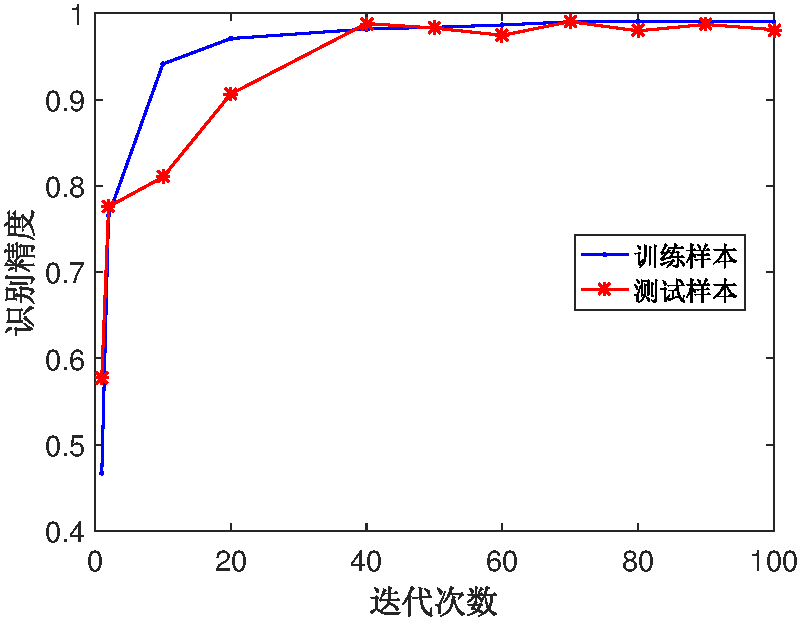
\includegraphics[width=6.67cm]{figures/emitter/diff_epoch}
		\caption{迭代次数与识别准确率曲线图}
		\label{fig:openset_epoch}
	\end{minipage}
	\hspace{10pt}
	\begin{minipage}{7cm}
		\centering
		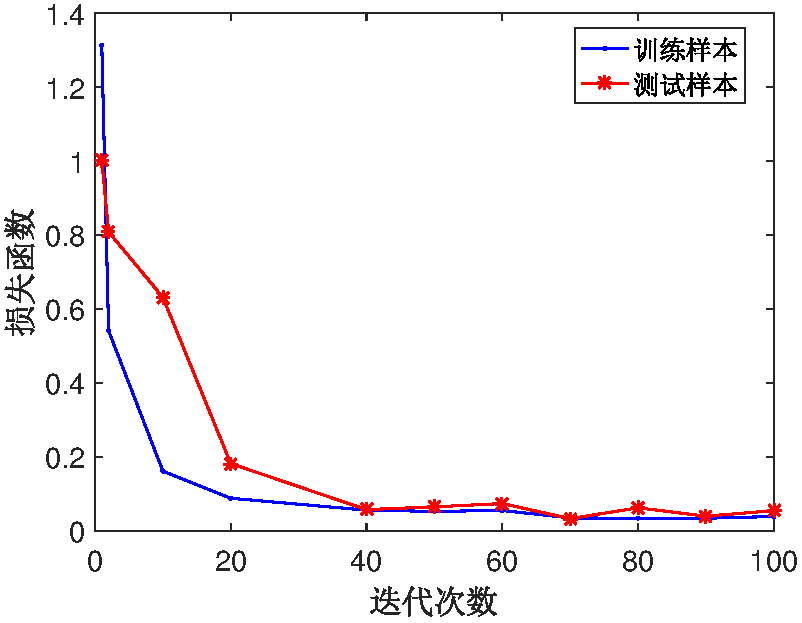
\includegraphics[width=6.67cm]{figures/emitter/diff_loss}
		\caption{迭代次数与损失函数曲线图}
		\label{fig:diff_loss}
	\end{minipage}

\end{figure}

\begin{table}[hbt]
	\renewcommand{\arraystretch}{1.3}
	\caption{深度卷积神经网络分类结果}
	% \label{tab:nb_classes}
	\centering\sWuhao
	\begin{tabular}{ccccccccc}
		\toprule
		 & 类别 A & 类别 B & 类别 C & 类别 D & 类别 E & 类别 F & 类别 G & 类别 H \\
		 \midrule
		% \multirow{8}{*}{正确分类精度}
		  类别 A & 100\% & 0 & 0 & 0 & 0 & 0 & 0 & 0 \\
		%  \cline{2-10}
		 类别 B & 7.42\% & 92.58\% & 0 & 0 & 0.13 & 0 & 0 & 0 \\
		% \cline{2-10}
		 类别 C & 0 & 0 & 97.83\% & 0 & 0 & 2.17\% & 0 & 0 \\
		% \cline{2-10}
		 类别 D & 0 & 0 & 3\% & 97\% & 0 & 0 & 0 & 0 \\
		% \cline{2-10}
		 类别 E & 0 & 0 & 0 & 0 & 100\% & 0 & 0 & 0 \\
		% \cline{2-10}
		 类别 F & 0 & 0 & 0.08\% & 0 & 0 & 99.92\% & 0 & 0 \\
		% \cline{2-10}
		 类别 G & 0 & 0 & 1.08\% & 0 & 0 & 0 & 98.92\% & 0 \\
		% \cline{2-10}
		 类别 H & 1.63\% & 0 & 0 & 0 & 0 & 0.63 & 0 & 98.37\% \\
		% \cline{2-10}
		\bottomrule
	\end{tabular}
\end{table}

\begin{table}[hbt]
	\renewcommand{\arraystretch}{1.3}
	\caption{深度卷积神经网络分类结果}
	% \label{tab:nb_classes}
	\centering\sWuhao
	% \begin{tabular}{p{1.5cm}p{2.6cm}p{2.6cm}p{2.6cm}p{2.6cm}p{1.6cm}}
		\begin{tabularx}{\textwidth}{>{\centering\arraybackslash}X>{\centering\arraybackslash}X>{\centering\arraybackslash}X>{\centering\arraybackslash}X}
		\toprule
		%  迭代次数 & 正确学习测试样本集个数 & 测试样本集学习正确率 & 正确学习训练样本集个数 & 训练样本集学习正确率 & 学习时间(s) \\
		迭代次数 & 训练样本学习正确率 & 测试样本学习正确率  &  学习时间(s) \\
		 \midrule
			1 & 0.4670 & 0.5782 & $1.0931\times 10^3$ \\
			2 & 0.7658 & 0.7758 & $2.3572\times 10^3$ \\
			10 & 0.9414 & 0.8102 & $1.1444\times 10^4$ \\
			20 & 0.9709 & 0.9065 & $2.1370\times 10^4$ \\
			40 & 0.9819 & 0.9883 & $4.3181 \times 10^4$ \\
			50 & 0.9839 & 0.9830 & $5.3437 \times 10^4$ \\
			60 & 0.9866 & 0.9746 & $6.4143 \times 10^4$ \\
			70 & 0.9903 & 0.9904 & $7.4849 \times 10^4$ \\
			80 & 0.9904 & 0.9798 & $8.5597 \times 10^4$ \\
			90 & 0.9908 & 0.9872 & $9.6328\times 10^4$ \\
			100 & 0.9902 & 0.9811 & $1.0711 \times 10^5$ \\
		\bottomrule
	\end{tabularx}
\end{table}


对于具有8个类别的数据,我们对于迭代次数与识别准确率进行了验证,其结果如图 \ref{fig:openset_epoch} 所示。
\subsubsection{Open Set 分类器识别结果}

在上述样本的情形下,我们通过选取不同的类别数目,进行训练和测试得到表\ref{tab:nb_classes}的识别结果。从表中数据我们可以看出,随着样本类别数的增加,对于未知分类的识别准确率也随之有了大幅度的增加,而另一方面随着类别的增加,对于每个类别的识别准确率仍然维持在比较高的水平。

% 此表格需要修改
\begin{table}[hbt]
	\renewcommand{\arraystretch}{1.3}
	\caption{不同已知类别个数数据识别结果}
	\label{tab:nb_classes}
	\centering\sWuhao
	\begin{tabularx}{\textwidth}{>{\centering\arraybackslash}X>{\centering\arraybackslash}X>{\centering\arraybackslash}X}
		\toprule
		 已知类别数目 & 已知类别识别正确率 & 未知类别分辨正确率 \\
		\midrule
		2 & 99.55\% & 84.32\% \\
		3 & 99.59\% & 93.10\% \\
		4 & 99.00\% & 97.81\% \\
		5 & 99.75\% & 98.42\% \\
		6 & 98.63\% & 98.85\% \\
		7 & 99.28\% & 99.22\% \\
		8 & 97.86\% & 99.14\% \\
		\bottomrule
	\end{tabularx}
\end{table}

% 对于本章这个Open Set 识别问题,我们需要用别的参数衡量识别的准确度。利用文\cite{scheirer2013toward}中提出的通过训练类别的个数和测试类别的个数来描述数据集的开放度(openness),如\equref{equ:openness}所示
% \begin{equation}
% 	openness = 1-\sqrt{\frac{2t}{\eta m+e}}
% 	\label{equ:openness}
% \end{equation}
% 其中,$t$表示训练类别的个数, $\eta $表示目标类别的个数,$m$ 表示分类器输出类别的个数,对于本章的识别问题,有$\eta=1$,$e$表示验证类别的个数,有$e>t,e>\eta$。对于一个完全的闭集识别问题有$e=t$意味着未知类别数据集为空。

% 另一方面,用F-measure 来衡量该分类器对于未知分类样本的处理情况。其定义为:
% \begin{equation}
% 	\text{F-measure}=2\times\frac{p\cdot r}{p+r}
% \end{equation}
% 其中,$p$表示精确率(precision),$p=\frac{TP}{TP+FP}$,其中$TP$表示正类识别为正类的样本数目,$FP$表示负类识别为正类的样本数目。$r$表示召回率(recall),$r=\frac{TP}{TP+FN}$,其中$FN$表示正类识别为负类的样本数目。

% openness 与 F-measure 曲线图

\section{小结}
本章针对复杂电磁环境下辐射源的识别面临的电磁信号干扰大、雷达信号参数相近等问题与挑战,利用深度学习的思想与方法,深入研究辐射源脉内细微特征,设计合适的神经网络结构,并基于民航机载气象雷达数据进行初步验证。主要特色与创新点如下:

(1)利用深度学习方法进行辐射源识别前沿。通过对现有辐射源信号进行分析,利用其脉内细微特征作为训练样本,使得识别准确率有了较大的进步。虽然已有研究利用神经网络、支持向量机等机器学习算法进行识别,但是仍然需要基于雷达信号的基本参数,没有考虑信号的内部特征参数。

(2)本章采用方法具有较强的抗噪声、抗干扰能力以及较好的鲁棒性。传统方法进行辐射源个体识别前均需进行降噪、多径抑制和分选等复杂的信号预处理工作,这些操作会在一定程度上削弱雷达的个体特征。深度学习方法可以通过大量的样本,智能地判断各特征的权重,通过赋予不同的权重在保留雷达个体特征的情况下,避免干扰的影响。

(3)本章设计了meta识别器,实现了对辐射源中未知分类的辨别。

% !Mode:: "TeX:UTF-8"

\chapter{基于深度学习的辐射源识别}
\label{sec:sei}
% TODO:增加内容与仿真!!!
% 对比利用不同的,添加具体参数的设置。


% 可以考虑进行未经过模糊函数处理和处理之后的对比

% 不同卷积核  学习率  不同卷积核个数
% 层数 节点数等
% 不同训练方法
% 多类别的分类结果图可以参考
% 不同数据的各自的图

\section{引言}
辐射源识别算法需要在无法收集大量数据的前提下正确的对目标进行分类并准确区分出已知目标和未知目标。
与传统利用已知类别的样本进行训练测试的机器学习算法不同,本章的问题是在Open Set的背景下,需要考虑输入未知分类样本的情况。
由于在复杂电磁环境下传统的辐射源个体识别面临识别能力差和无法识别未知目标等问题与挑战,因此需要寻找一种新的方法解决该问题。

本章综合雷达信号处理、深度学习等多学科理论,通过对实际数据的分析,结合深度卷积神经网络与支持向量机方法,以雷达信号的模糊函数切片作为训练样本的特征向量,构建了一个可以对未知分类进行辨识的分类器。最后,利用数据进行验证,证明本章提出的分类器具有很高的准确性。

本章安排如下: \ref{sec:sei_data}节对辐射源信号进行了分析,并对其进行预处理,求取其模糊函数切片,\ref{sec:sei_method}节构建了本章的Open Set 分类器,详细地阐述了深度卷积神经网络主分类器与支持向量机Meta-Recognition的设计过程,\ref{sec:sei_experiment}节利用数据对分类器已知分类识别和未知分类辨别的性能进行了验证,\ref{sec:sei_summary}节进行本章总结。

\section{辐射源信号分析}
\label{sec:sei_data}
对辐射源信号的分析处理,本章主要考虑两方面:信号预处理、特征提取优化。
本章所获得的信号为雷达辐射源的I/Q两路数据,这是一种在雷达信号处理领域常见的用来描述信号的方法。其中I表示In-Phase,即同相;Q表示Quadrature,即正交,与I相位之差为90度。
设需要表示的信号的峰值幅度为$A$、相位角为$\phi$,则有:
\begin{equation}
	I = A\cos{\phi},
	\label{equ:i}
\end{equation}
\begin{equation}
	Q = A\sin{\phi}.
	\label{equ:q}
\end{equation}
也即可以利用\equref{equ:signal}表示信号:
\begin{equation}
	Ae^{i\phi}=A(\cos(\phi) + i\sin(\phi))=I+Qi.
	\label{equ:signal}
\end{equation}
从而可以根据\equref{equ:i}和\equref{equ:q}利用I/Q数据求取信号的峰值幅度和相位角:
\begin{equation}
	A=\sqrt{I^2+Q^2},
\end{equation}
\begin{equation}
	\phi=tan^{-1}(Q/I).
\end{equation}
在完成信号形式的转换后,首先需要对信号进行初步的预处理,剔除无用和错误的数据。
在特征提取优化方面,合理的特征是分类识别的基础。由于存在相同型号的辐射源,利用简单的参数特征无法很好的完成辐射源的个体识别,但是在实际中辐射源自身存在相位噪声以及各类杂散输出,此部分特征可以用来区分出型号、参数均相同的辐射源,因此需要选取一种可以提取雷达辐射源这种无意调制产生的信号脉内细微特征的方法。
% 模糊函数不仅能描述辐射源信号的分辨特性与模糊度,还能描述由雷达辐射源信号所决定的测量精度、杂波抑制特性等,
通过模糊函数在时延和频偏这两个维度上的变换,可以多角度的刻画出无意调制对发射信号的影响,因此本章最终选取了利用雷达模糊函数挖掘辐射源的特征。
\subsection{模糊函数}
信号$x(t)$的瞬时自相关函数为$R_x(t,\tau)=x(t+\tau/2)x^{*}(t-\tau/2)$,其中$\tau$为时延,模糊函数的定义为,
\begin{equation}
A(\tau,\nu) = \int_{-\infty}^{+\infty}R_x(t,\tau)e^{j2\pi\nu t}dt,
\label{equ:defineaf}
\end{equation}
即$R_x(t,\tau)$关于时间$t$的傅里叶反变换。

为了方便在数字信号中使用,\equref{equ:defineaf}可以经过变换等价于\equref{equ:afcon}的形式:
\begin{equation}
A(\tau,\nu) = \int_{0}^{\tau}x(t)x^{*}(t+\tau)e^{j2\pi\nu t}dt.
\label{equ:afcon}
\end{equation}
对信号均匀采样,即对接收信号和参考信号离散化后,\equref{equ:afcon}可以表示为:
\begin{equation}
A(\tau_l,\nu_m) = A(l, m) = \sum_{n = 0}^{N-1}x(n)x^{*}(n+l)e^{\frac{j2\pi m n}{N}},
\end{equation}
其中,$\tau_l=l/f_s$、$\nu_m=mf_s/N$。

此处以一个简单的单载频矩形脉冲信号来展示模糊函数特征提取的作用,图\ref{fig:danpinmaichong}为模糊函数图,可以发现模糊函数存在一定的冗余,其主要变化均处于0时偏和0频偏附近。
为了减小计算量,本章在频偏为0附近取不同时间延迟的切片作为信号特征,可以有效地提取信号的相位噪声和杂散输出等个体特征,并且此处受噪声的干扰较小,更加稳定。图 \ref{fig:qiepian}即为在频偏为0处的单载频矩形脉冲信号模糊函数切片。

\begin{figure}[hbt]
	\centering
	\begin{minipage}[b][][b]{7cm}
		\centering
		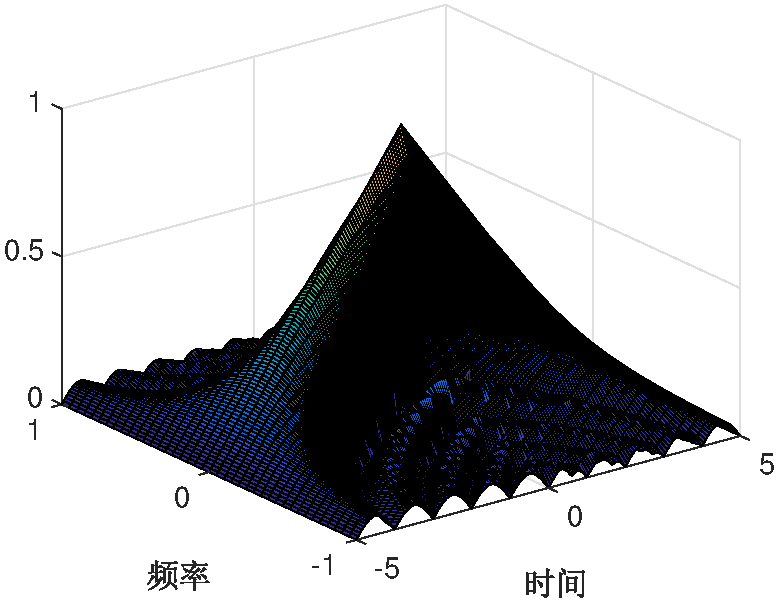
\includegraphics[width=6.67cm]{figures/emitter/danpinmaichong}
		\caption{单载频矩形脉冲信号模糊函数图}
		\label{fig:danpinmaichong}
	\end{minipage}
	\hspace{10pt}
	\begin{minipage}[b][][b]{7cm}
		\centering
		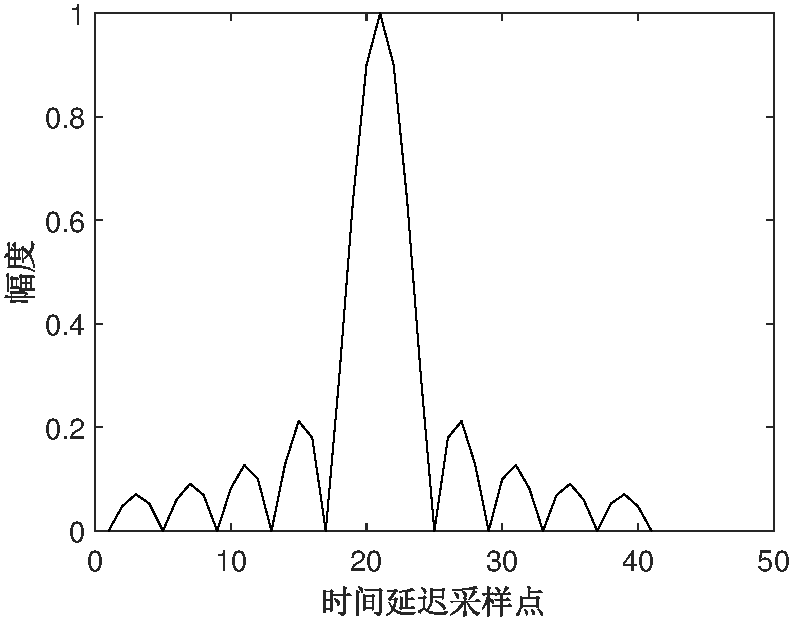
\includegraphics[width=6.67cm]{figures/emitter/qiepian}
		\caption{单载频矩形脉冲信号模糊函数切片}
		\label{fig:qiepian}
	\end{minipage}

\end{figure}

\section{Open Set 分类器设计}
\label{sec:sei_method}
通常的识别或者分类系统仅考虑的是一个闭集分类系统,然而在现实世界中,这种分类系统会遇到很大的问题。由于其最基本的假设是所有的类别均为先验已知,那么就会出现问题,例如在训练样本中不存在类别的样本就会被错误的分到某个类别中去。这种在训练过程提供不完整的信息,而在测试时添加未知分类的问题,称作Open Set识别\ucite{scheirer2013toward, jain2014multi}。该问题还可以描述为需要在测试过程中拒绝未知样本,Open Set目标识别系统必须可以准确的处理以下三种类型的数据类:
\begin{itemize}
	\item 已知的(目标)类,被标注为正训练样本的数据,
	\item 已知的未知(非目标)类,被标注为负训练样本的数据,
	\item 未知的未知(非目标)类,在训练样本中不存在的类别的数据。
\end{itemize}
传统的机器学习算法均是针对闭集数据设计的,随着识别算法应用场景的增多和对精度要求的提高,许多学者开始了对Open Set识别的研究。Simonson\ucite{simonson1998probabilistic}提出了一种称作概率融合(probabilistic fusion, PF)的利用统计的方法来进行Open Set识别,其主要通过合并来自不同数据源的证据得到一个统计测试模型,根据此模型的分布来对类别进行判断。Scheirer等人\ucite{scheirer2011meta}提出了一种通过分析后验数据得分来进行类型判断的方法。

此部分主要解决的问题是当得到一个新的测试样本,如果该样本不属于已经经过训练的分类,那么传统的神经网络模型会将该样本指派给与其最相似的一个类别,此种情况对一个Open Set识别系统,也即类似于辐射源识别系统这种具有较多尚未经过训练的样本的一个数据集,首先这会导致其识别率下降,另一方面是由于对未知辐射源无法很好的确定,无法很好的完成预警等任务。
目前,学者对该问题的研究主要有两个思路:
\begin{itemize}
	\item 在训练集中添加一个“未知”类别,利用不同的来自非已知类别的数据作为训练样本对该类别进行训练,然后对所有的输入数据进行类别的识别,将识别结果为该类别的数据作为未知分类数据。
	\item 针对多分类使用的softmax函数,可以设立阈值或者对该识别结果进行一个评价(例如与已知类别数据的一个“距离”),通过这种方式分辨出未知分类。
\end{itemize}
第一个思路最大的问题是实际工程中无法得到所有可能的未知类别的样本来进行训练,具有一定的局限性,不适用于本章这个具有大量来自未知分类数据的问题。针对该问题,本章基于后一个思路设计了一个基于Meta-Recognition的可以识别未知辐射源的深度神经网络。首先是创建一个深度卷积神经网络分类器,该分类器的输出为该训练样本属于各个类别的概率,然后将此类别作为一个输入,输入到一个支持向量机分类器Meta-Recognition中,然后利用该Meta-Recognition判断输入是否为未知分类。
\begin{figure}[hbt]
	\centering
	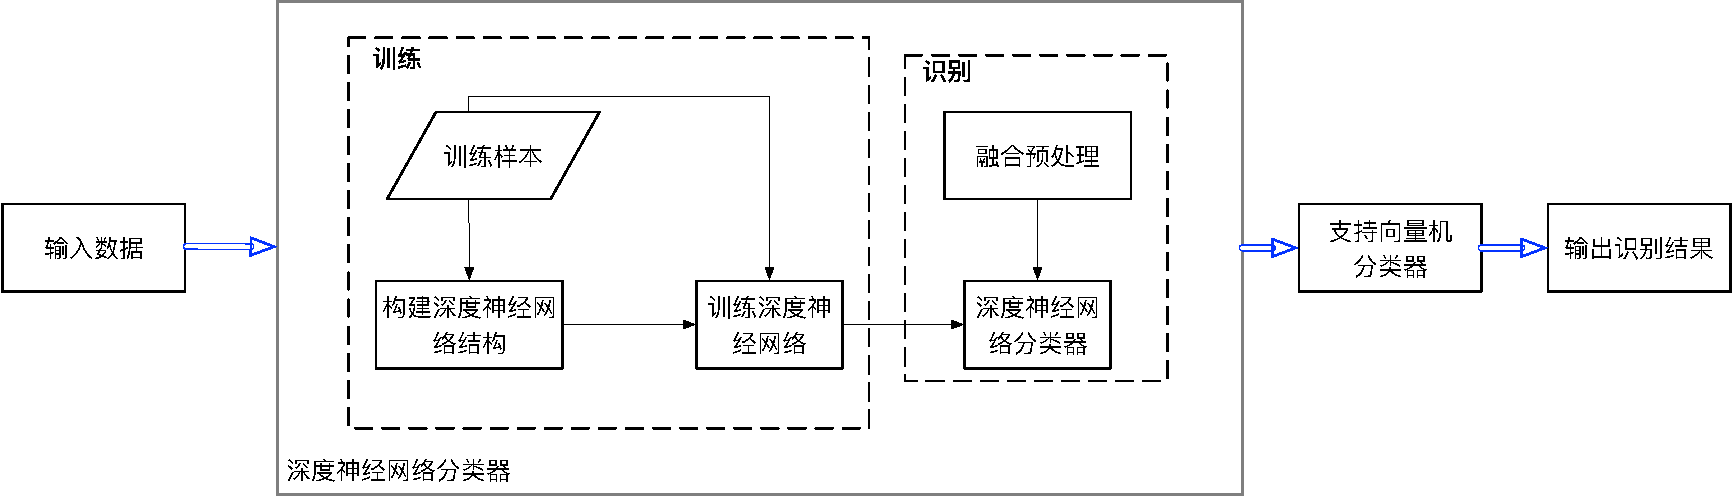
\includegraphics[width=13.5cm]{figures/emitter/frame_emitter}
	\caption{分类器设计结构图}
\end{figure}

\subsection{深度卷积神经网络分类器设计}
本章根据辐射源信号的实际数据以及其反映出来的特性,设计了一个如图\ref{fig:struct_emitter}所示具有10层的一维卷积神经网络。
该分类器作为主分类器,且Meta-Recognition是以该分类器的输出作为输入,所以该分类器性能的好坏会直接影响到对已知类别的分类和对未知类别的判断。

第一层是输入层,由于模糊函数切片为一个$1 \times 1000$的向量,因此输入层大小是$1 \times 1000$。

第二层是卷积层$C1$,$C1$对输入向量进行一维卷积运算提取特征,卷积运算可以最
大程度的提取原始信号的特征。此处利用了256个大小为$1\times 3$的卷积滤波器,其窗口移动步长为1。

第三层是一个池化层$S2$,$S2$层对上一层$C1$做池化处理,此处采用的是$1\times 2$的最大池化操作。
% 池化的目的是在保留数据有用信息的同时,尽可能减少数据量。 %--查重去掉

第四层是一个卷积层 $C3$,$C3$对$S2$的特征进行卷积操作,此处利用了128个大小为$1\times 3$的卷积滤波器。

第五层是一个卷积层 $C4$,其结构与$C3$相同,128个大小为$1\times 3$的卷积滤波器。

第六层是一个池化层 $S5$,其结构与$S2$相同,$1\times 2$的最大池化操作。

第七层是一个卷积层 $C6$,其结构与$C3$相同,128个大小为$1\times 3$的卷积滤波器。

第八层是一个卷积层 $C7$,其结构与$C3$相同,128个大小为$1\times 3$的卷积滤波器。

第九层是一个池化层 $S8$,其结构与$S2$相同,$1\times 2$的最大池化操作。

第十层是输出层,根据不同的类别个数选取相应的输出节点个数,首先将$S8$的特征拉成一个一维向量,然后通过全连接网络与输出层进行连接,通过Softmax激活函数输出最终的结果。

\begin{figure}[hbt]
	\centering
	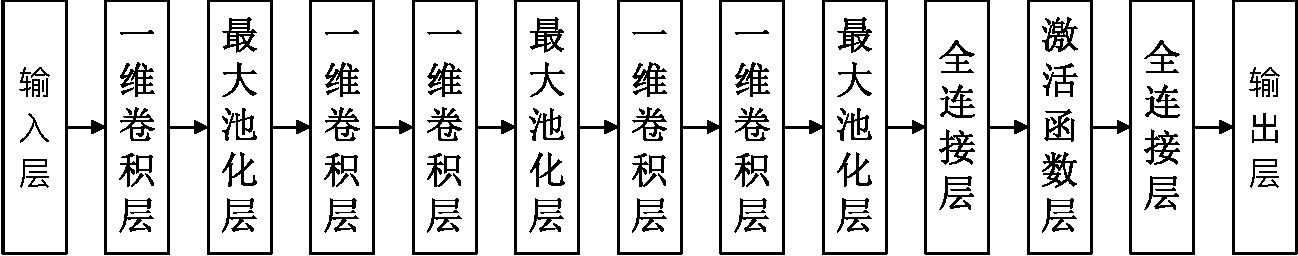
\includegraphics[width=13.5cm]{figures/emitter/struct_emitter}
	\caption{深度卷积神经网络框架图}
	\label{fig:struct_emitter}
\end{figure}

\subsection{支持向量机 Meta-Recognition 设计}

\subsubsection{支持向量机原理}
支持向量机是一种流行的分类方法,它可以在不需要大量数据的情况下产生良好的结果。对一个二分类问题,设$((x_1,y_1),\dots,(x_n,y_n))$为训练数据集,其中$x_i$为某样本的特征向量,$y_i\in\{-1,+1\}$为该样本的标签。支持向量机的思想为找到一个超平面将这些样本划分为正类(标签为$+1$)和负类(标签为$-1$),并且使得正类和负类之间的距离最大,该超平面的间隔被定义为正类与负类之间的最近距离。

对于一个线性分类问题,假设所有数据均满足约束:
\begin{equation}
\begin{array}{cc}
	w\cdot x_i +b \geq + 1 \quad y_i &= +1, \\
	w\cdot x_i +b \leq + 1 \quad y_i &= -1,
	\label{equ:constraint}
\end{array}
\end{equation}
其中$w$为超平面的法向量,$\frac{|b|}{||w||}$是从超平面到原点的垂直距离,$||w||$是向量$w$的欧拉范数。将上述两个式子合并得到:
\begin{equation}
	y_i(w\cdot x_i+b)\geq 1 \forall i
	\label{equ:svm}
\end{equation}
\equref{equ:svm} 中的训练样本构成了图 \ref{fig:hyperplanes} 中的分类平面$H_1$与$H_2$,间隔 $\rho$ 可以通过计算$H_1$与$H_2$的距离得到:
\begin{equation}
	\rho=\frac{|1-b|}{||w||}-\frac{|-1-b|}{||w||}=\frac{2}{||w||}.
\end{equation}
\begin{figure}[hbt]
	\centering
	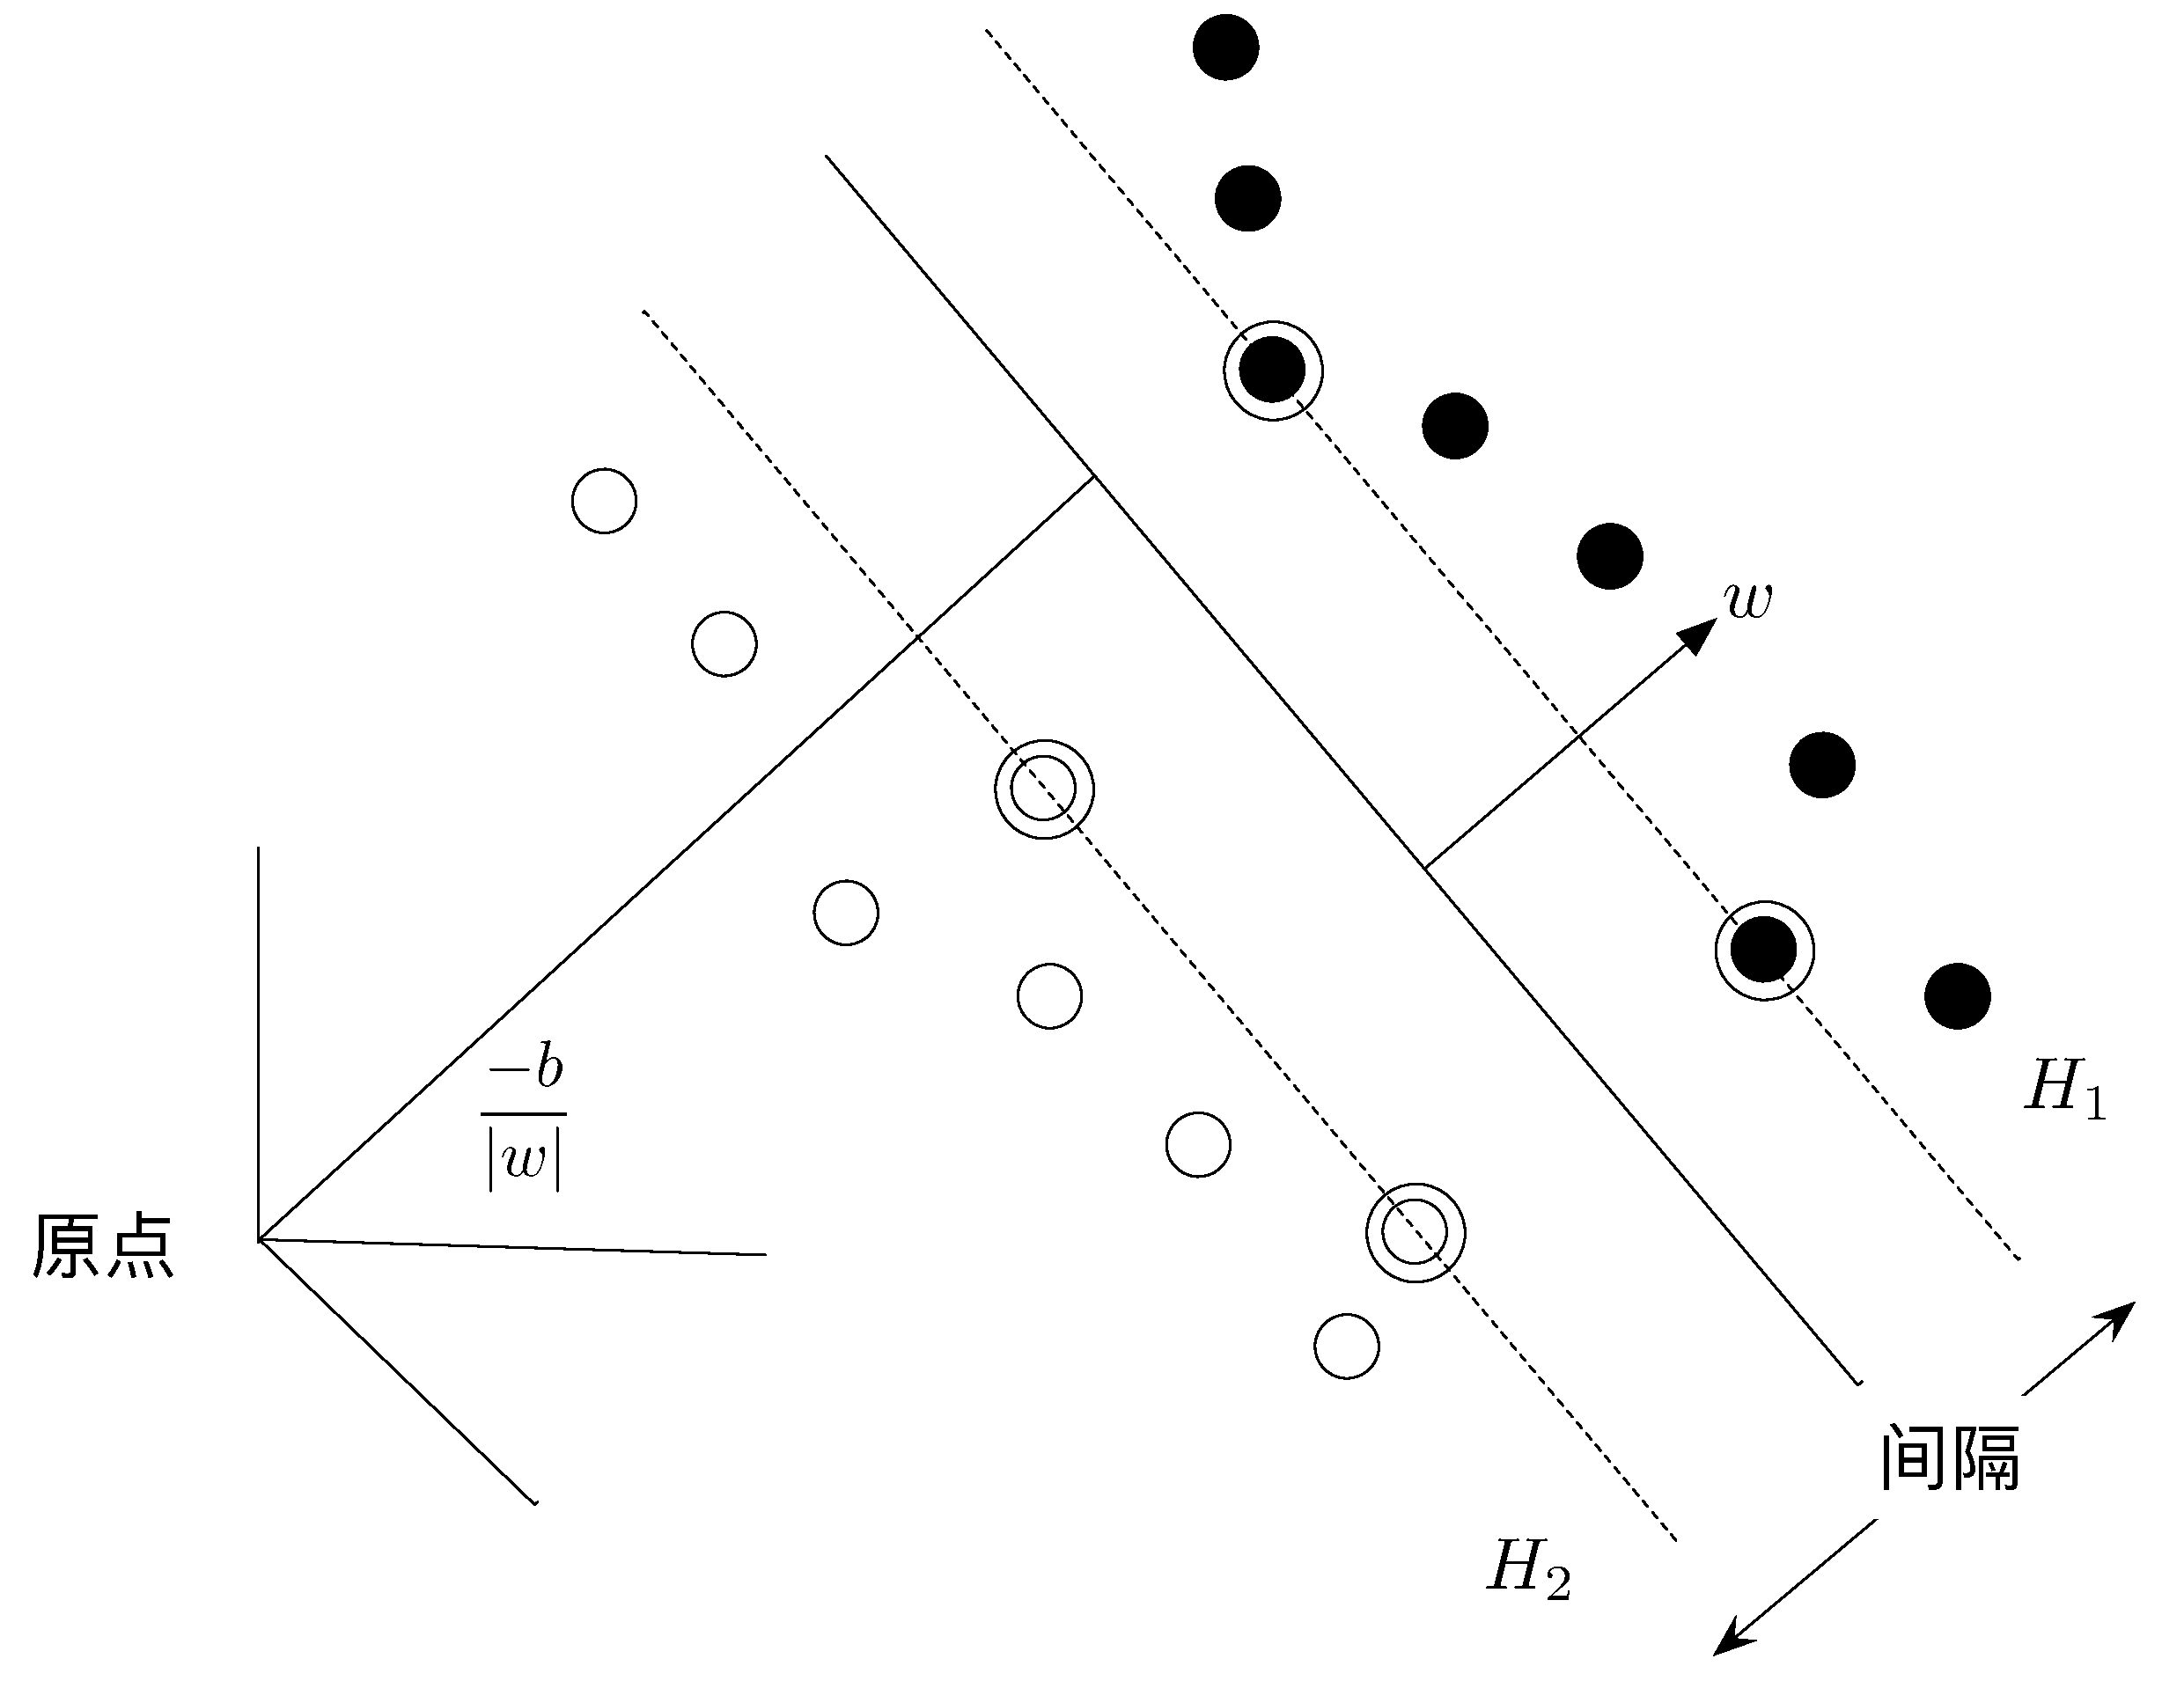
\includegraphics[width=6.67cm]{figures/emitter/svm_hard}
	\caption{标准分类平面,即具有最大间隔的超平面。被圈起来的样本组成超平面,这些样本被称作支持向量。}
	\label{fig:hyperplanes}
\end{figure}
因此求解标准分类超平面的最大间隔的问题,就转变为一个优化问题:
\begin{equation}
	\min \limits_{w\in \mathcal{H}} \tau(w)=\frac{1}{2}||w||^2\quad s.t. \quad y_i(w\cdot x_i +b) \geq 1 \quad \forall i
	\label{equ:optimization}
\end{equation}
为了更好表示约束,可以用拉格朗日优化算法对\equref{equ:optimization}重新表示:
\begin{equation}
	\min \limits_{w,b} L(w,b,\alpha)=\frac{1}{2}||w||^2-\sum_{i=1}^l\alpha_i y_i (x_i w + b) + \sum_{i=1}^l{\alpha_i},
	\label{equ:lagrange}
\end{equation}
其中$\alpha_i \geq 0$为约束条件。

在实际计算过程中,可以通过对偶定义求解优化方程\equref{equ:lagrange},通过最大化方程\equref{equ:lagrange}相对于$\alpha$来求取其相对于$w$和$b$的最小值。利用 Karush-Kuhn-Tucker 条件,\equref{equ:lagrange}变为对偶形式:
\begin{equation}
	\max \limits_{\alpha} L_D=\sum_i{\alpha_i}-\frac{1}{2}\sum_{i,j}\alpha_i\alpha_jy_iy_jx_i\cdot x_j \quad s.t. \quad \forall i
	\left\{
		\begin{aligned}
	   &\sum_i{\alpha_iy_i}=0  \\
	   &\alpha_i \geq 0
	   \end{aligned}
		\right.
\end{equation}
因此,通过求解该对偶优化问题,可以得到系数$\alpha_i$,其中满足$\alpha_i>0$的解称作支持向量,他们位于标准分类平面$H_1$或者$H_2$上。注意到,仅有$\alpha_i>0$的解影响最终的支持向量的选择。
因此,可以得到决策函数:
\begin{equation}
	f(x)=w^Tx_i+b=\sum_{i=1}^My_i\alpha_i(x_i^Tx)+b.
\end{equation}
决策函数的符号取决于预测样本$x$。

此处讨论的情形的一个假设是可以把所有样本完全分为不同的类别。但是显然在大多数情况下,这种假设是不成立的。另外,这种假设也会导致过拟合现象的出现。因此,文献 \cite{cortes1995support} 提出了软间隔的支持向量机。
其主要思想是通过引入正的松弛变量$\xi_i$放宽\equref{equ:constraint}的约束,从而得到:
\begin{equation}
	\forall i \quad
	\left\{
	 \begin{aligned}
	&w\cdot x_i + b \geq +1-\xi_i \quad y_i=+1  \\
	&w\cdot x_i + b \leq -1-\xi_i \quad y_i=+1  \\
	&\xi_i \geq 0
	\end{aligned}
	 \right.
	\label{equ:constraint_soft}
\end{equation}
这允许一些样本在边缘内部,甚至在相反类别的情况下进一步交叉(见图\ref{fig:softmargin})。 虽然这种松弛使得支持向量机能够灵活地降低异常值的影响,但是从优化问题求解的角度来看,任意大的松弛变量$\xi_i$可能会导致SVM获得平凡解或次优解。 因此,可以通过使松弛变量成为\equref{equ:optimization}的一部分,来限制松弛度:
\begin{equation}
	\min \limits_{w\in \mathcal{H},\xi\in \mathbb{R}^m} \tau(w,\xi)=\frac{1}{2}||w||^2+C\sum_{i=1}^m {\xi_i}
\end{equation}
\begin{figure}[hbt]
	\centering
	\includegraphics[width=6.67cm]{figures/emitter/svm_soft}
	\caption{软间隔支持向量机}
	\label{fig:softmargin}
\end{figure}
其约束条件为\equref{equ:constraint_soft}。超参数$C>0$是针对误分类的惩罚系数,该系数需要根据不同的分类任务和数据集进行调整,
将其变为对偶形式:
\begin{equation}
	\max \limits_{\alpha} L_D=\sum_i{\alpha_i}-\frac{1}{2}\sum_{i,j}\alpha_i\alpha_jy_iy_jx_i\cdot x_j \quad s.t. \quad \forall i
	\left\{
		\begin{aligned}
	   &\sum_i{\alpha_iy_i}=0  \\
	   &C \leq \alpha_i \geq 0
	   \end{aligned}
		\right.
	\label{equ:cdotdual}
\end{equation}
目前只是分析了线性支持向量机的问题,为了应对非线性分类问题,引入了核函数的概念。
将训练数据通过某函数$\Phi:\mathbb{R}^d\mapsto\mathcal{H}$,经过该变换后,只需要将原来计算$\mathbb{R}^d$的$x_i\cdot x_j$ 变为计算在$\mathcal{H}$域的向量积$\Phi(x_i)\cdot\Phi(x_j)$。为了降低计算量,可以引入核函数$K$来避免数据$x_i$和$x_j$从$\mathbb{R}^d$映射到$\mathcal{H}$:
\begin{equation}
	K(x_i,x_j)=\Phi(x_i)\cdot\Phi(x_j).
\end{equation}
因此,可以将\equref{equ:cdotdual}变为:
\begin{equation}
	\max \limits_{\alpha} L_D=\sum_i{\alpha_i}-\frac{1}{2}\sum_{i,j}\alpha_i\alpha_jy_iy_j K(x_i,x_j)\quad s.t. \quad \forall i
	\left\{
		\begin{aligned}
	   &\sum_i{\alpha_iy_i}=0  \\
	   &C \leq \alpha_i \geq 0
	   \end{aligned}
		\right.
\end{equation}
常用的核函数有下面几种:
\begin{itemize}
	\item 线性核函数:$K(x,y)=x^Ty+C$
	\item 多项式核函数:$K(x,y)=(x^Ty+C)^d$
	\item RBF 核函数:$K(x,y)=e^{\frac{-||x-y||^2}{2\sigma^2}}$
	\item Sigmoid 核函数:$K(x,y)=\tanh(\alpha x^Ty+C)$
\end{itemize}
% \subsubsection{支持向量机设计}
% 本章设计的支持向量机分类器以深度卷积神经网络的输出作为输入,利用各类别的概率作为特征进行训练识别。
% 由于在类别的识别过程中存在一定的波动性,其会影响结果是否属于未知类别的辨别,因此本章选取来自同一个辐射源连续10拍的识别结果平均作为最终的输入。

% 支持向量机分类器的设计主要分为核函数的选择和参数的选择两方面。核函数将输入空间映射到高维特征空间,最终在高维特征空间中构造出最优分类超平面,从而把平面上本身不好分的非线性数据分开。常用的核函数为线性核函数和径向基核函数( Radial Basis Function, RBF)。在核函数的选择方面,当特征数量很大时一般选用线性核函数,而对本章这种特征数量比较小的问题,一般选择径向基核函数。

% 具有径向基核的支持向量机具有两个关键参数,惩罚参数$C$的和核参数$\sigma$,这两个参数的取值在很大程度上决定了SVM的性能的优劣。
% 核参数$\sigma$主要影响样本数据在高维特征空间中分布的复杂程度,即维数。特征子空间的维数越高,那么得到的最优分类超平面就会越复杂。因此只有选择合适的核参数得到合适的特征子空间,才能得到泛化能力良好的SVM分类器。大量的实验数据表明,如果与样本点之间的距离很小,$\sigma \rightarrow 0$;如果与样本点之间的距离很大时,$\sigma \rightarrow \infty$。当$\sigma$很小,径向基核函数支持向量机得到的判别函数差不多是一个常数,出现过拟合现象;当$\sigma$很大时,样本的正确分类率也会比较低。

% 惩罚参数是影响SVM算法性能的另一个重要因素。它的作用主要是调节特征子空间中SVM模型的置信范围与经验风险的比例,使支持向量机的泛化能力达到最好。当特征子空间不同时,最优参数值取值也会不同。惩罚参数与经验误差的惩罚和SVM的复杂度成正比,与经验风险值成反比。因此,选择合适的惩罚参数也是非常重要的。

\section{仿真实验与分析}
\label{sec:sei_experiment}
\subsection{实验环境}

本章利用了来自13架民航飞机的气象雷达辐射源的数据,飞机信息参见表\ref{tab:flight}
\begin{table}[hbt]
	\renewcommand{\arraystretch}{1.3}
	\caption{辐射源信号数据}
	\label{tab:flight}
	\centering\sWuhao
	\begin{tabularx}{\textwidth}{>{\centering\arraybackslash}X>{\centering\arraybackslash}X>{\centering\arraybackslash}X}
		\toprule
		 飞机地址码 & 飞机航班号 & 飞机型号  \\
		 \midrule
		 7BF014 & CCA1416 & Airbus A330 (twin-jet)\\
		 780DB3 & TBA9881 & Airbus A330 (twin-jet) \\
		 780E06 & CSN3438 & Airbus A330 (twin-jet\\
		 780EBB & CES293 & 	Airbus A321 (twin-jet)\\
		 780EBF & CES2342 & Airbus A320 (twin-jet)\\
		 7804F2 & ZH9164 & Airbus A320 (twin-jet)\\
		 7804F4 & CES5856 & Boeing 737\\
		 7806FC & CSN6402 & Airbus A320 (twin-jet)\\
		 7808F0 & CES5373 & Airbus A319 (twin-jet)\\
		 78057F & CCA4103 & Airbus A321 (twin-jet\\
		 780063 & CCA4377 & Airbus A319 (twin-jet)\\
		 780375 & CSC8253 & Airbus A319 (twin-jet)	\\
		 781022 & EU2731 & Airbus A319 (twin-jet)\\
		 \bottomrule
	\end{tabularx}
\end{table}

本章利用的数据是机载气象雷达辐射源信号,原始的雷达信号是如图 \ref{fig:IQ} 所示的I/Q信号,
为了更好的捕捉到雷达辐射源回波的特征信息,本章对数据进行了一个变换,利用快速傅里叶变换求取其模糊函数,并取偏移为0附近的一个切片作为输入的特征向量,经过变换后的样本的特征如图\ref{fig:diff_data}所示。
\begin{figure}[hbt]
	\centering
	\begin{minipage}{7cm}
		\centering
		\includegraphics[width=6.67cm]{figures/emitter/IQA}
		\caption{原始I/Q信号}
		\label{fig:IQ}
	\end{minipage}
	\hspace{10pt}
	\begin{minipage}{7cm}
		\centering
		\includegraphics[width=6.67cm]{figures/emitter/diff_data}
		\caption{不同类别样本特征图}
		\label{fig:diff_data}
	\end{minipage}
\end{figure}
由于该变换后,数据之间的差距比较大,为了通过线性变换将原始数据映射到$[0 , 1]$之间
本章对数据利用离差标准化(Min-Max Normalization)方法进行归一化,
转换函数如下:
\begin{equation}
x^{*}=\frac{x-x_{min}}{x_{max}-x_{min}},
\end{equation}
其中$x_{max}$为样本数据的最大值,$x_{min}$为样本数据的最小值。

在数据的选择方面,本章从全部数据中选择出2至8个类别分别进行实验,每一个类别的原始信号为100次雷达扫描周期的信号。
由于深度学习需要大量的数据进行训练学习,而本身数据量偏少,故本章在已有数据的基础上在一定信噪比的前提下,生成部分仿真数据,最终每架飞机均有10000组信号。本章选择全部数据的$70\%$作为训练样本,$20\%$用于交叉验证,$10\%$作为测试,同时在测试样本中添加与其等量的来自未训练类别也即未知类别的样本共同作为测试样本用来衡量其未知分类的识别率。
本章采用网格搜索法对SVM参数进行调优,最终选择参数惩罚参数为$C=32$,核参数$\sigma=0.0312$。

\subsection{实验结果分析}

\subsubsection{深度卷积神经网络识别结果}

首先验证深度卷积算法的识别正确率,利用8个类别的数据进行训练和测试,迭代次数为100次,其分类结果如表\ref{tab:cnn_29}所示。从表格中容易看出,每一个单独类别的分类精度都很高。
\begin{table}[hbt]
	\renewcommand{\arraystretch}{1.3}
	\caption{深度卷积神经网络分类结果}
	\label{tab:cnn_29}
	\centering\sWuhao
	\begin{tabular}{ccccccccc}
		\toprule
		 & 类别 A & 类别 B & 类别 C & 类别 D & 类别 E & 类别 F & 类别 G & 类别 H \\
		 \midrule
		 类别 A & 100\% & 0 & 0 & 0 & 0 & 0 & 0 & 0 \\
		 类别 B & 7.42\% & 92.58\% & 0 & 0 & 0.13 & 0 & 0 & 0 \\
		 类别 C & 0 & 0 & 97.83\% & 0 & 0 & 2.17\% & 0 & 0 \\
		 类别 D & 0 & 0 & 3\% & 97\% & 0 & 0 & 0 & 0 \\
		 类别 E & 0 & 0 & 0 & 0 & 100\% & 0 & 0 & 0 \\
		 类别 F & 0 & 0 & 0.08\% & 0 & 0 & 99.92\% & 0 & 0 \\
		 类别 G & 0 & 0 & 1.08\% & 0 & 0 & 0 & 98.92\% & 0 \\
		 类别 H & 1.63\% & 0 & 0 & 0 & 0 & 0.63 & 0 & 98.37\% \\
		\bottomrule
	\end{tabular}
\end{table}

同对迭代次数与识别准确率和损失函数进行了验证,在CPU为i5-3.30GHz、运存为1GB的Linux虚拟机运行本章的算法程序,其结果如图 \ref{fig:openset_epoch}、图\ref{fig:diff_loss}和表\ref{tab:cnn_epoch_29}所示,无论是训练样本还是测试样本,其精度与损失函数均很快收敛到比较好的水平,不过相应的学习时间也正比增长,故在实际工程中需要对精度和时间进行衡量选取一个最合适的迭代次数。
\begin{table}[hbt]
	\renewcommand{\arraystretch}{1.3}
	\caption{深度卷积神经网络分类结果}
	\label{tab:cnn_epoch_29}
	\centering\sWuhao
		\begin{tabularx}{\textwidth}{>{\centering\arraybackslash}X>{\centering\arraybackslash}X>{\centering\arraybackslash}X>{\centering\arraybackslash}X}
		\toprule
		迭代次数 & 训练样本学习正确率 & 测试样本学习正确率  &  学习时间(s) \\
		 \midrule
			1 & 0.4670 & 0.5782 & $1.0931\times 10^3$ \\
			2 & 0.7658 & 0.7758 & $2.3572\times 10^3$ \\
			10 & 0.9414 & 0.8102 & $1.1444\times 10^4$ \\
			20 & 0.9709 & 0.9065 & $2.1370\times 10^4$ \\
			40 & 0.9819 & 0.9883 & $4.3181 \times 10^4$ \\
			50 & 0.9839 & 0.9830 & $5.3437 \times 10^4$ \\
			60 & 0.9866 & 0.9746 & $6.4143 \times 10^4$ \\
			70 & 0.9903 & 0.9904 & $7.4849 \times 10^4$ \\
			80 & 0.9904 & 0.9798 & $8.5597 \times 10^4$ \\
			90 & 0.9908 & 0.9872 & $9.6328\times 10^4$ \\
			100 & 0.9902 & 0.9811 & $1.0711 \times 10^5$ \\
		\bottomrule
	\end{tabularx}
\end{table}

\begin{figure}[hbt]
	\centering
	\begin{minipage}{7cm}
		\centering
		\includegraphics[width=6.67cm]{figures/emitter/diff_epoch}
		\caption{迭代次数与识别准确率曲线图}
		\label{fig:openset_epoch}
	\end{minipage}
	\hspace{10pt}
	\begin{minipage}{7cm}
		\centering
		\includegraphics[width=6.67cm]{figures/emitter/diff_loss}
		\caption{迭代次数与损失函数曲线图}
		\label{fig:diff_loss}
	\end{minipage}
\end{figure}
\subsubsection{Open Set 分类器识别结果}

在上述样本的情形下,可以通过选取不同的类别数目,进行实验得到表\ref{tab:nb_classes}的识别结果。
从表中可以看出,随着样本类别数的增加,未知分类的识别准确率也随之有了大幅度的增加,同时每个类别的识别准确率仍然维持在比较高的水平。

\begin{table}[hbt]
	\renewcommand{\arraystretch}{1.3}
	\caption{不同已知实验类别个数数据识别结果}
	\label{tab:nb_classes}
	\centering\sWuhao
	\begin{tabularx}{\textwidth}{>{\centering\arraybackslash}X>{\centering\arraybackslash}X>{\centering\arraybackslash}X}
		\toprule
		 已知实验类别数目 & 已知类别识别正确率 & 未知类别分辨正确率 \\
		\midrule
		2 & 99.55\% & 84.32\% \\
		3 & 99.59\% & 93.10\% \\
		4 & 99.00\% & 97.81\% \\
		5 & 99.75\% & 98.42\% \\
		6 & 98.63\% & 98.85\% \\
		7 & 99.28\% & 99.22\% \\
		8 & 97.86\% & 99.14\% \\
		\bottomrule
	\end{tabularx}
\end{table}

\section{小结}
\label{sec:sei_summary}
本章针对复杂电磁环境下辐射源的识别面临的电磁信号干扰大、雷达信号参数相近等问题与挑战,利用深度学习的思想与方法,深入研究辐射源脉内细微特征,设计合适的深度卷积神经网络结构和支持向量机Meta-Recognition,实现了对辐射源中未知分类的辨别。基于民航机载气象雷达数据对本章提出的方法进行初步验证,表明该方法具有较强的抗噪声、抗干扰能力以及较好的鲁棒性。
% 传统方法进行辐射源个体识别前均需进行降噪、多径抑制和分选等复杂的信号预处理工作,这些操作会在一定程度上削弱雷达的个体特征。通过对现有辐射源信号进行分析,深度学习方法利用其脉内细微特征作为训练样本,使得识别准确率有了较大的进步。

\chapter{总结}
\section{本文的主要贡献}
雷达信号分类一直是雷达领域一个很重要的方面,通过对接受到的信号的分类识别,可以更好的了解战场形势。在电子科技迅猛发展的今天,电磁环境急剧变化,雷达信号分类在军事侦查、目标识别、电子对抗等领域有着广阔的应用场景。
而深度学习方法由于其在识别分类等领域的结果,引起了国内外越来越多学者的重视。本文对于雷达信号分类中的两个方面进行了研究,通过对雷达信号数据的分析,构建合理的卷积神经网络模型,实现了对于雷达信号类别的识别。同时,针对于识别过程中存在未知类别的情况,构建了一个支持向量机分类器作为Meta-Recognition进行二次识别,实现了未知分类的辨别。本文的主要研究成果和最终的结论如下:

本文首先综述了深度学习的研究现状和发展,以及其与传统神经网络方法相比的优点所在。描述了深度学习的几种常用方法和基本结构,研究了深度卷积神经网络的原理和其训练过程。

针对于天波超视距雷达中由于电离层的变化无法确定其坐标配准系数的问题,本文通过地海杂波识别进行地理位置匹配来获取该变换系数,用于提高目标定位精度。在地海杂波识别过程中,通过对于海量频谱数据的分析,构建了一个一维卷积神经网络分类器。同时将该算法的识别结果与传统的基于信号频谱分析和支持向量机算法进行对比,证明了本文算法的优越性。

对于辐射源识别中未知分类的辨别问题,首先概述了辐射源识别中雷达信号处理的过程,介绍了辐射源特征提取和辐射源识别的常用方法及存在的问题。本文将深度学习和支持向量机相结合,构建了用于辐射源分类及未知分类辨别的模型,通过实际数据进行实验验证,并对不同辐射源类别数、卷积神经网络层数、节点数、不同支持向量机参数与正确率进行了比较,讨论了相关参数对结果的影响。

\section{后续的研究进展}
在本文中,我们利用实际数据进行测试并验证了我们的深度学习方法在地海杂波识别方法和辐射源识别这两个方面的有效性。但是由于雷达数据处理方面信号种类多,在实际工程中涉及环节多,因此,对于利用深度学习进行雷达信号处理还有很多工作需要完成。结合本文所研究的问题,我们希望未来可以在以下方面做进一步研究:
\begin{itemize}
	\item 针对于雷达信号特征,对本文算法进一步调整。在天波雷达地海杂波识别中,我们现在把已有数据分成几组,分别进行训练。我们计划尝试使用一些方法对这些数据进行融合分析,以获得一个可以适应各种数据情况的模型。对于辐射源识别,利用更多的数据对算法进行进一步的验证,目前类别较少的情况下,部分结果会对选择的类别具有一定的依赖性,另一方面是选取更多更合适的特征进行训练学习。
	\item 进一步优化算法,提高计算效率。虽然在数据量比较大的情况下,深度学习算法具有准确率高的优势,但训练过程计算量较大。本文拟将深度学习方法同其他方法进行结合,进一步完善网络结构,降低计算量、提高训练速度。
	\item 进一步优化网络结构、相关参数的选取、训练方法等。深度学习的理论研究仍然存在一些不足,可以通过进一步的理论研究,选择更加优秀的参数和训练方法。除了本文的卷积神经网络结构之外,我们计划尝试其他深度学习的方法或者思想来解决我们的问题或者构建更优的神经网络结构。
	\item 对数据进行无监督或者半监督学习的方式进行训练。由于雷达信号量大,人为进行标记困难较大,本文计划进一步尝试无监督等减少人为标记的工作量。
	\item 本文目前的工作更偏重于工程应用,对于深度学习相关理论知识的研究不足,后续需要增强理论知识的研究。
\end{itemize}


\backmatter

\bibliographystyle{nputhesis}
\bibliography{references/reference,references/emitter}

% \Appendix
% \phantomsection
\chapter*{附~~~~录}

\addcontentsline{toc}{chapter}{\fHei 附录}

附录附录附录附录附录附录附录附录附录附录附录附录附录附录附录附录附录附录附录附录附录附录附录附录附录附录附录附录附录附录附录附录附录附录附录附录附录附录附录附录附录附录附录附录附录附录附录附录附录附录附录附录附录附录附录附录附录附录附录附录附录附录附录附录附录附录附录附录附录附录附录附录附录附录附录附录附录附录附录附录附录附录附录附录附录附录附录附录附录附录附录附录附录附录附录附录附录附录附录附录附录附录附录附录附录附录附录附录附录附录附录附录附录附录附录附录附录附录附录附录附录附录附录附录附录附录附录附录附录附录附录附录附录附录附录附录附录附录附录附录附录附录附录附录附录附录附录附录附录附录附录附录附录附录附录附录附录附录附录附录附录附录附录附录附录附录附录附录附录附录附录附录附录附录附录附录附录附录附录附录附录附录附录附录附录附录附录附录附录附录附录附录附录附录附录附录附录附录附录附录附录附录附录附录附录附录附录附录附录附录附录附录附录附录附录附录附录附录附录附录附录附录附录附录附录附录附录附录附录附录附录附录附录附录附录附录附录附录附录附录附录附录附录附录附录附录附录附录附录附录附录附录附录附录附录附录附录附录附录附录附录附录附录附录附录附录附录附录附录附录附录附录附录附录附录附录附录附录附录附录附录附录附录附录附录附录附录附录附录附录附录附录附录附录附录附录附录附录附录附录附录附录附录附录附录附录附录附录附录附录附录附录附录附录附录附录附录附录附录附录附录附录附录附录附录附录附录附录附录附录附录附录附录附录附录附录附录附录附录附录附录附录附录附录附录附录附录附录附录附录附录附录附录附录附录附录附录附录附录附录附录附录附录附录附录附录附录附录附录附录附录附录附录附录附录附录附录附录附录附录附录附录附录附录附录附录附录附录附录附录附录附录附录附录附录附录附录附录附录附录附录附录附录附录附录附录附录附录附录附录附录附录附录附录附录附录附录附录附录附录附录附录附录附录附录附录附录附录附录附录附录附录

附录附录附录附录附录附录附录附录附录附录附录附录附录附录附录附录附录附录附录附录附录附录附录附录附录附录附录附录附录附录附录附录附录附录附录附录附录附录附录附录附录附录附录附录附录附录附录附录附录附录附录附录附录附录附录附录附录附录附录附录附录附录附录附录附录附录附录附录附录附录附录附录附录附录附录附录附录附录附录附录附录附录附录附录附录附录附录附录附录附录附录附录附录附录附录附录附录附录附录附录附录附录附录附录附录附录附录附录附录附录附录附录附录附录附录附录附录附录附录附录附录附录附录附录附录附录附录附录附录附录附录附录附录附录附录附录附录附录附录附录附录附录附录附录附录附录附录附录附录附录附录附录附录附录附录附录附录附录附录附录附录附录附录附录附录附录附录附录附录附录附录附录附录附录附录附录附录附录附录附录附录附录附录附录附录附录附录附录附录附录附录附录附录附录附录附录附录附录附录附录附录附录附录附录附录附录附录附录附录附录附录附录附录附录附录附录附录附录附录附录附录附录附录附录附录附录附录附录附录附录附录附录附录附录附录附录附录附录附录附录

附录附录附录附录附录附录附录附录附录附录附录附录附录附录附录附录附录附录附录附录附录附录附录附录附录附录附录附录附录附录附录附录附录附录附录附录附录附录附录附录附录附录附录附录附录附录附录附录附录附录附录附录附录附录附录附录附录附录附录附录附录附录附录附录附录附录附录附录附录附录附录附录附录附录附录附录附录附录附录附录附录附录附录附录附录附录附录附录附录附录附录附录附录附录附录附录附录附录附录附录附录附录附录附录附录附录附录附录附录附录附录附录附录附录附录附录附录附录附录附录附录附录附录附录附录附录附录附录附录附录附录附录附录附录附录附录附录附录附录附录附录附录附录附录附录附录附录附录附录附录附录附录附录附录附录附录附录附录附录附录附录附录附录附录附录附录附录附录附录附录附录附录附录附录附录附录附录附录附录附录附录附录附录附录附录附录附录附录附录附录附录附录附录附录附录附录附录附录附录附录附录附录附录附录附录附录附录附录附录附录附录附录附录附录附录附录

\clearpage
\endinput
\ifx\final\undefined

\else
    \Thanks

    \if\final1
        % !Mode:: "TeX:UTF-8"

时光荏苒,光阴似箭。两年多的研究生生涯即将结束,我的校园生活也即将画上句号。研究生阶段的生活和本科时候,发生了很大的变化,实验室给提供了更加优异的环境,让我可以学习到更多的知识。

首先,我要感谢我的导师潘泉老师。虽然和潘老师接触的时间有限,但是每次和潘老师交流都给我很大的帮助。潘老师宽广的视野总是能一针见血的发现问题所在,让我深受启发。潘老师对学术的热情和认真的态度一直鼓励着我用最严谨的态度进行学习和工作,他渊博的学识、开阔的思维以及循循善诱的教学方法让我深受裨益。

在硕士期间,王增福老师和兰华老师对我的指导十分重要。两位老师在学术研究与工程实践方面都给予了我很多帮助和指导。两位老师渊博的学识、严谨的治学态度、活跃的学术思想以及温厚的为人,让我受益匪浅。两位老师谆谆的教诲和一丝不苟的指导,是我终身受益的宝贵财富。同时还要感谢实验室杨峰老师、焦连猛老师等众位老师的无私帮助和辛勤栽培。

感谢实验室给予了一个温暖的环境,感谢史志远博士、胡玉梅博士、孙帅硕士、戴安东硕士、张婷婷硕士、祝志勇硕士、马季容硕士、孙藏安硕士、王家琦硕士等实验室的各位师兄、师姐、师弟、师妹,可以帮助我解决各种学术与生活中的问题,与大家的讨论使得我可以更加深入的理解问题,而科研之余的丰富多彩的活动也帮助我劳逸结合。

其次,感谢含辛茹苦的父母多年来对我学业和生活上的关心、支持和理解,没有你们就没有我的今天。感谢李毅兰同学,多年的陪伴使得我成长为一个更加优秀的人。

最后还要感对我的论文进行评审和指导的各位专家老师!
    \else
        时光荏苒,光阴似箭。两年多的研究生生涯即将结束,我的校园生活也即将画上句号。研究生阶段的生活和本科时候,发生了很大的变化,实验室给提供了更加优异的环境,让我可以学习到更多的知识。

首先,我要感谢我的导师xx老师。虽然和x老师接触的时间有限,但是每次和潘老师交流都给我很大的帮助。x老师宽广的视野总是能一针见血的发现问题所在,让我深受启发。x老师对学术的热情和认真的态度一直鼓励着我用最严谨的态度进行学习和工作,他渊博的学识、开阔的思维以及循循善诱的教学方法让我深受裨益。

在硕士期间,xxx老师和xx老师对我的指导十分重要。两位老师在学术研究与工程实践方面都给予了我很多帮助和指导。两位老师渊博的学识、严谨的治学态度、活跃的学术思想以及温厚的为人,让我受益匪浅。两位老师谆谆的教诲和一丝不苟的指导,是我终身受益的宝贵财富。同时还要感谢实验室杨峰老师、焦连猛老师等众位老师的无私帮助和辛勤栽培。

感谢实验室给予了一个温暖的环境,感谢xxx博士、xxx博士、xx硕士、xxx硕士、xxx硕士、xxx硕士、xxx硕士、xxx硕士、xxx硕士等实验室的各位师兄、师姐、师弟、师妹,可以帮助我解决各种学术与生活中的问题,与大家的讨论使得我可以更加深入的理解问题,而科研之余的丰富多彩的活动也帮助我劳逸结合。

其次,感谢含辛茹苦的父母多年来对我学业和生活上的关心、支持和理解,没有你们就没有我的今天。感谢xxx同学,多年的陪伴使得我成长为一个更加优秀的人。

最后还要感对我的论文进行评审和指导的各位专家老师!
    \fi

    \Work
    % \section{dfad}
% \centerline{\textbf{\Large{作者硕士期间完成的文章及其他研究成果}}}
\begin{enumerate}
\item 第一作者,发明专利,一种基于深度学习的雷达辐射源类别识别方法,受理号:201711145195.9
\item 第二作者,国防专利,一种天波超视距雷达地海杂波类型识别方法,受理号:201718003477.X

\item 第二作者,国防专利,一种天波超视距雷达多目标自动跟踪方法,受理号:201618010431.6

\item 第二作者,Control Conference (CCC),2016 35th Chinese,Controller design for anti-heeling system in container ships,DOI: 10.1109/ChiCC.2016.7554263

\item 第二作者,International Radar Symposium 2017,Random Sample Consensus Algorithm for Multiple Target Tracking in Over-the-horizon Radar,DOI: 10.23919/IRS.2017.8008099

\item 第二作者,Sea/Land Clutter Recognition for Over-The-Horizon Radar via Deep Convolution Neural Network,Under Review

\item 第三作者,国防专利,一种天波超视距雷达多目标跟踪联合检测与跟踪方法,受理号:201618001893.1

\item 第二作者,软件著作权:LIFT\underline{\hspace{0.5em}}基于变分贝叶斯的多目标联合检测与跟踪软件,登记号:2016R11S233158

\item 第五作者,国防专利,一种基于置信传播的多路径数据关联方法,受理号:201618001088.9

\item 第五作者,IEEE Journal of Selected Topics in Signal Processing,Joint Detection and Tracking for Multipath Targets: A Variational Bayesian Approach,Under Review

\item 主要完成人,天波超视距雷达地海杂波识别与舰船目标跟踪性能提升技术研究,南京14所合作项目

\end{enumerate}

% \centerline{作者硕士期间参与的项目}

    \statement

\fi
\end{document}

